\documentclass[11pt]{article}
\usepackage{amsfonts}
\usepackage{amsmath}
\usepackage{xcolor}

\usepackage{enumitem}

\usepackage{graphicx}
\graphicspath{{./images/}}
\usepackage{sidecap}

\usepackage{hyperref}

\usepackage{listings}
\usepackage{fancybox}

\lstset{
  basicstyle=\ttfamily,
  breaklines=true,
  postbreak=\mbox{\textcolor{red}{$\hookrightarrow$}\space},
  numbers=left,
  stepnumber=1,
  numberstyle=\tiny,
  tabsize=1,
  keywordstyle=\color{blue}\ttfamily,
  stringstyle=\color{red}\ttfamily,
  commentstyle=\color{gray}\ttfamily,
  morecomment=[l][\color{magenta}]{\#},
  frame=shadowbox
}

\usepackage[margin=3cm]{geometry}

\usepackage{float}
\usepackage{algorithm}
\usepackage{algpseudocode}

\title{Real-Time Procedural Terrain Generation with Marching Cubes}
\author{}
\date{}

\setcounter{tocdepth}{3}

\begin{document}

% \bibliographystyle{plainurl}
\bibliographystyle{plainurl}

\maketitle
\begin{figure}[H]
  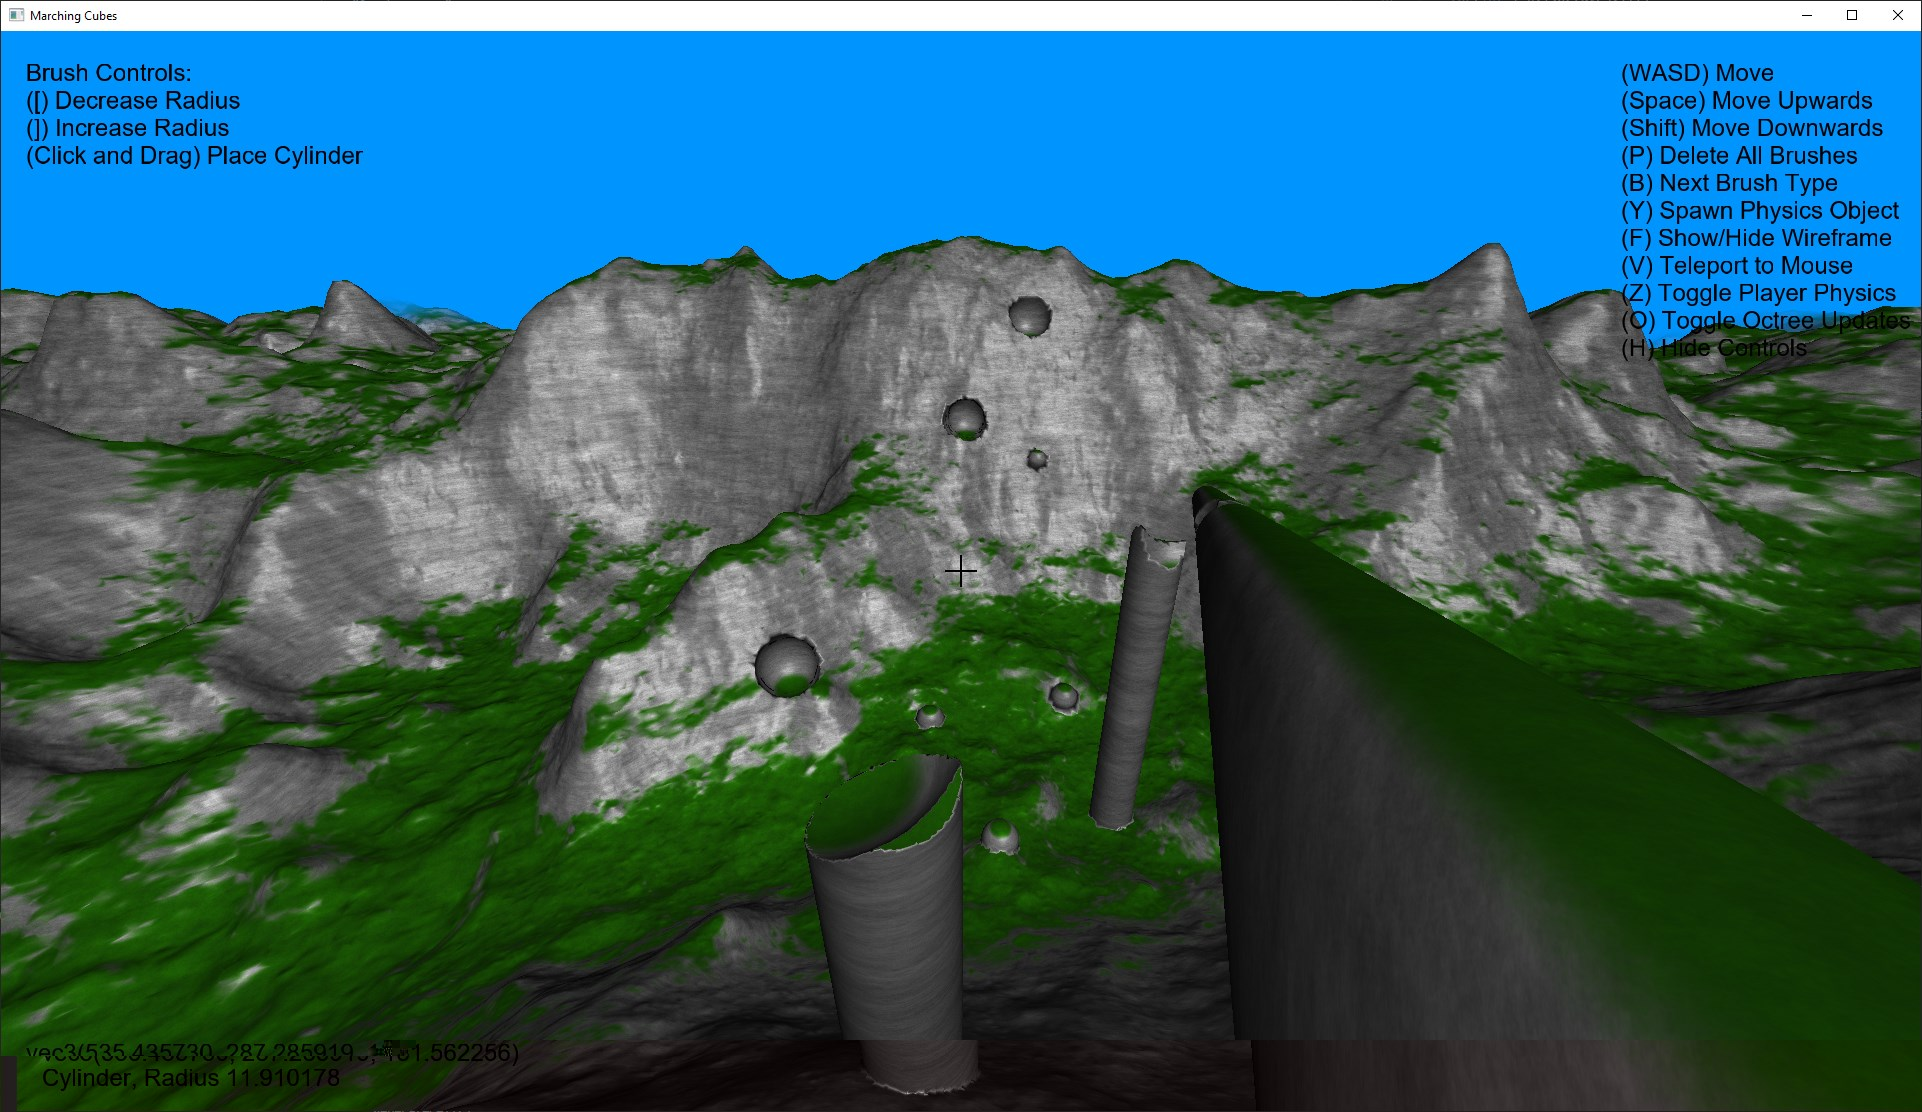
\includegraphics[width=\textwidth]{shaded_mountains.jpg}
\end{figure}
\newpage

\section*{Abstract} 
This project explores a method for procedurally generating terrain by applying a variation of Marching Cubes known as Transvoxel. We use an octree data structure to break down a large world into chunks at varying levels of detail, and apply parallel processing on the GPU to rapidly generate geometry on a per-chunk basis. We explore applications of this approach, modifying geometry in real-time by making localized changes to the underlying distance function. Finally, we use the generated meshes with a well-known physics library, and apply procedural shading.
\newpage

\tableofcontents

\newpage
\section{Introduction} 

Marching Cubes is an algorithm for polygonising a scalar field. Designed by William E. Lorensen and Harvey E. Cline in 1987~\cite{10.1145/37402.37422}, the original application was in medical imaging, to create anatomical models using data from 3D scans such as CT scans. When it was written, the algorithm was comparatively expensive to execute, due to the limited hardware available. 

Procedural terrain generation is a popular technique within the video game industry, allowing for large areas of geometry to be created, according to mathematical rules, rather than the traditional method of 3D modelling, which is time-consuming for the modeller, and takes up a large amount of storage space.

The increase in processing power available, as well as the parallel design of the GPU, means that it is achievable to use Marching Cubes to procedurally generate large amounts of geometry at an interactive framerate. When combined with a level-of-detail system, it is possible to render very large regions of terrain, that can be interacted with and modified in real time.

\section{Background}
\subsection{Signed Distance Functions} 
\label{section:sdf}
To pass a scalar field to the Marching Cubes algorithm, we will use a signed distance function (SDF). This is a function of the form $f:\mathbb{R}^3 \rightarrow \mathbb{R}$. The shape represented by an SDF is the implicit surface $f\left(x,y,z\right) = 0$. An SDF should have the following properties:
\begin{enumerate}[label=\roman*.]
\item If $\left(x,y,z\right)$ is inside the surface, $f\left(x,y,z\right) < 0$. If $\left(x,y,z\right)$ is outside the surface, $f\left(x,y,z\right) > 0$. This is the defining property of an SDF, without which Marching Cubes will not produce valid geometry.
\item $f\left(x,y,z\right)$ represents the smallest (signed) euclidean distance from the point $\left(x,y,z\right)$ to the surface. Many functions we are using do not give the exact distance, however for best results the value should be a good approximation, and for floating point precision reasons, must be at least the same order of magnitude. This property is used to interpolate the positions of vertices, and as such the accuracy of the distance approximation impacts the accuracy of the generated surface. An SDF such that $f\left(x,y,z\right)$ gives the correct distance everywhere is an \textit{exact} SDF. Otherwise, it is an \textit{approximate} SDF.
\item Near the surface, $f$ is continuous, and has all first partial derivatives. This is useful since the gradient of an SDF on the surface gives the normal vector to the surface at that point.
\end{enumerate}

An article by Inigo Quilez lists some useful SDFs~\cite{quilez:sdf}. Figures \ref{fig:Circle_SDF} and \ref{fig:Hill_SDF} show some examples.

\begin{SCfigure}[][!h]
\caption{2 dimensional exact SDF representing a circle. The SDF shown is $f\left(x,y\right)=\sqrt{x^2+y^2}-1$, with the area where $f\left(x,y\right)<0$ shaded. Also shown are the contours where $f\left(x,y\right)=0.1,0.2,...0.5$. At the center point $\left(0,0\right)$, the gradient is undefined. However, since this point is not close to the surface, $f$ can still be used as an SDF without issue.}
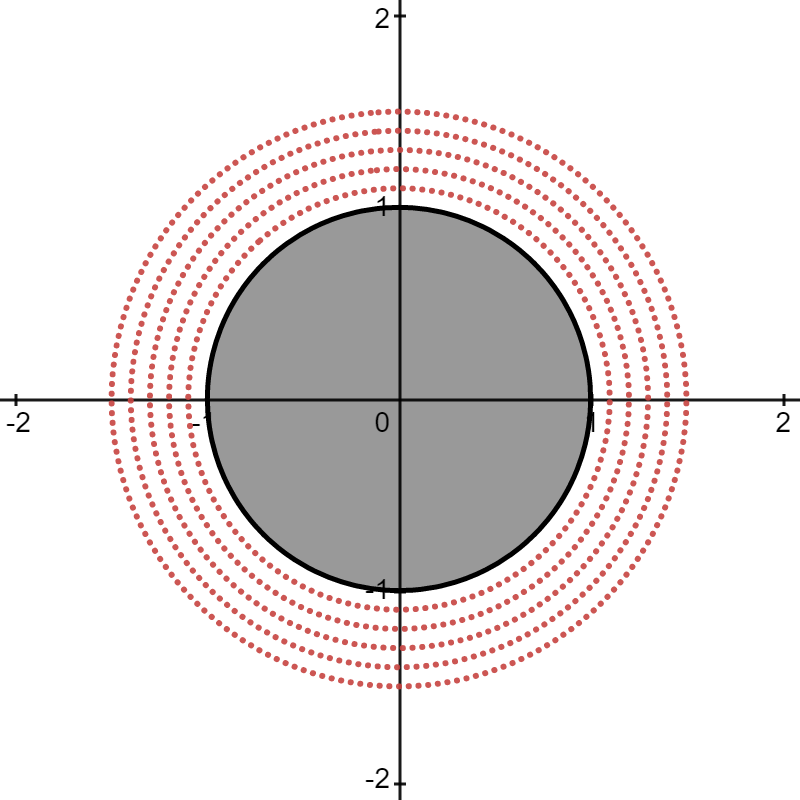
\includegraphics[width=0.5\textwidth]{Circle_SDF}
\label{fig:Circle_SDF}
\end{SCfigure}


\begin{SCfigure}[][!h]
\caption{2 dimensional approximate SDF for the curved surface defined by $f\left(x,y\right)=y-\left(1-\frac{x^2}{3}\right)$. The contour lines are no longer uniformly spaced, as they would be with an exact SDF.}
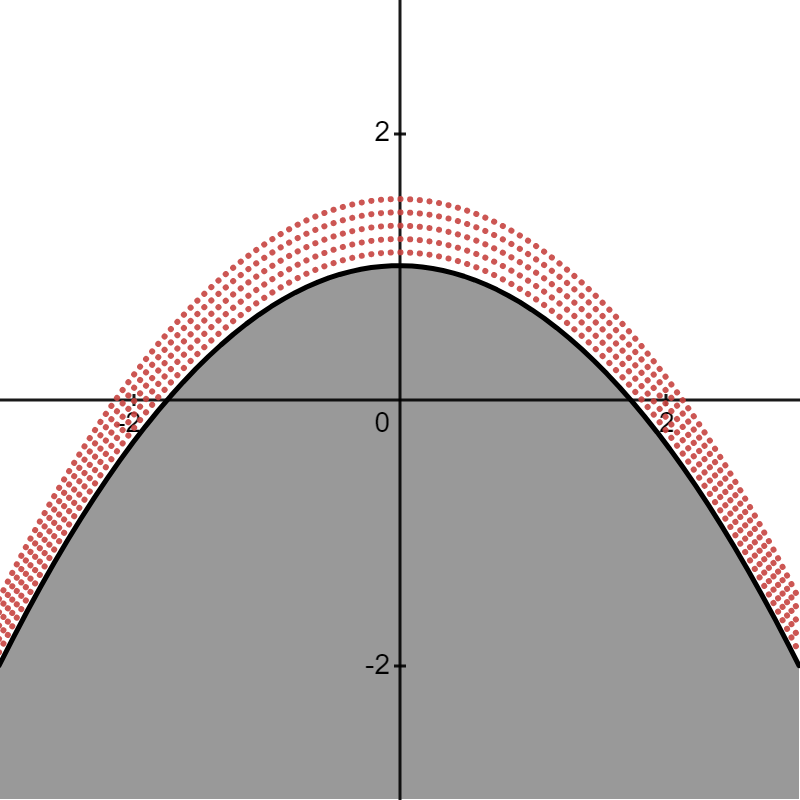
\includegraphics[width=0.5\textwidth]{Hill_SDF}
\label{fig:Hill_SDF}
\end{SCfigure}

Many shapes have an exact SDF that is complex to evaluate, so it is more efficient to use an approximate SDF instead. We will see an example of this in section \ref{example_brushes}.

The set-theoretical operations of union, intersection, and difference have representations using the $\min$ and $\max$ functions. Where the function $\min\left(f,g\right)$ is not differentiable at the point where $f = g$, we choose the derivative of either $f$ or $g$. Using these functions, it is possible to combine SDFs of many shapes to produce a surface that is more complex.

\subsection{Noise}
\label{section:noise}
Use of noise to create natural-looking heightmaps is a commonly used technique. A noise function assigns a pseudorandom value in the range $\left[0,1\right]$ to each point in $\mathbb{R}^n$. We will consider coherent noise, which has the property that input values that are far apart will produce random-looking outputs, but input values that are close together will result in similar output. This means that the function is smooth. One such function is value noise, which assigns a pseudorandom value to each grid point, and then smoothly interpolates between these values to assign a value to every point. Multiple layers or \textit{octaves} of value noise at different scales can be added together to produce fractal noise. More advanced noise algorithms exist, such as Perlin or Simplex noise~\cite{PerlinChapter2N}, that show fewer regularities. Figures \ref{fig:value_noise} and \ref{fig:better_noise} show some example noise functions.

\begin{SCfigure}[][!h]
  \caption{Left: A single layer of value noise. Right: 8 octaves of value noise.}
  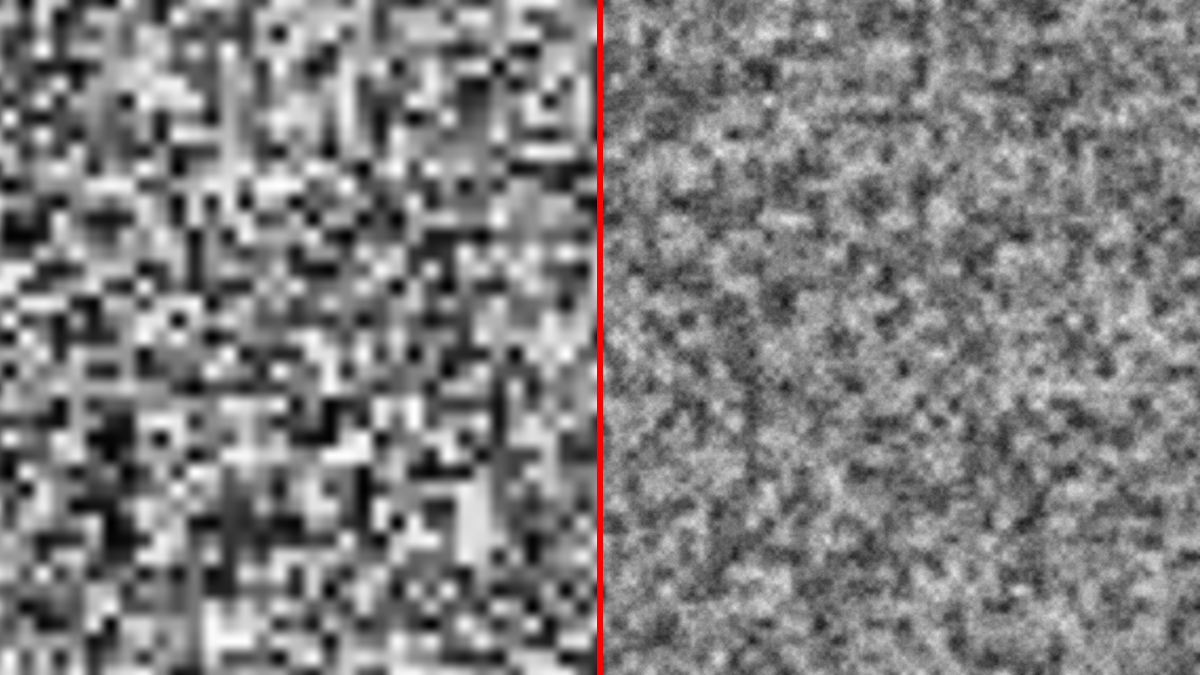
\includegraphics[width=0.5\textwidth]{value_noise.png}
  \label{fig:value_noise}
\end{SCfigure}

\begin{SCfigure}[][!h]
  \caption{Left: Perlin Noise. Right: Simplex Noise. Images generated using functions \texttt{cnoise} and \texttt{snoise} respectively, from the cited collection of reference implementations~\cite{github_2014}.}
  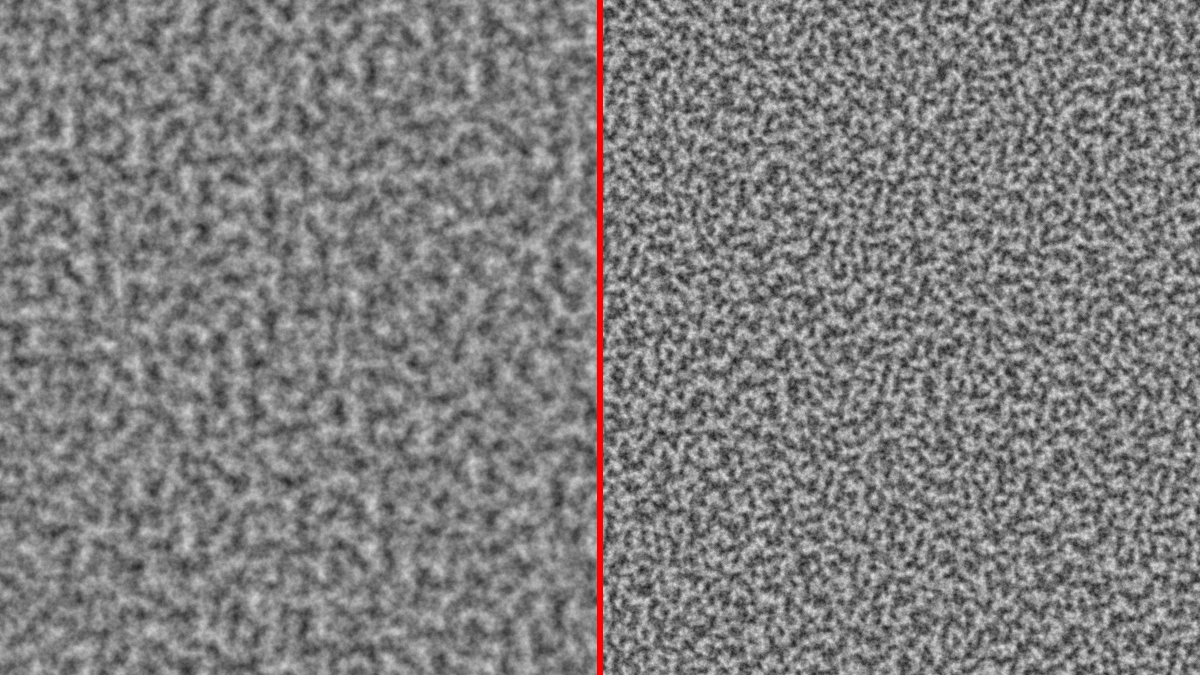
\includegraphics[width=0.5\textwidth]{better_noise.png}
  \label{fig:better_noise}
\end{SCfigure}

The output of a noise function can be scaled to define a convincing heightmap, typically giving a function $y = h\left(x,z\right)$ defining the height of the terrain at a given $\left(x,z\right)$ coordinate. We will extend this to an approximate SDF, using the formula $f\left(x,y,z\right) = y - h\left(x,z\right)$. In this case, the distance approximation worsens as the steepness of the slope of $h\left(x,z\right)$ increases.
\\
It is also possible to use a 3D noise function in an SDF, for example in generating features such as caves. By defining a value at which the surface will be, for example $0.5$, we can use the SDF $f\left(x,y,z\right) = \mathrm{noise}\left(x,y,z\right) - 0.5$ to represent a shape such that only points with noise values greater than 0.5 are outside of the shape. With careful choices of parameters, this creates empty pockets throughout the shape. We will use this type of SDF for benchmarking purposes, since it generates a relatively large amount of geometry, and represents a shape that cannot be created using a heightmap approach. 

\subsection{Marching Cubes Algorithm}
\label{section:mc}
Marching Cubes is an algorithm for polygonising a 3 dimensional scalar field. It works by splitting the space into a uniform grid of cubes (\textit{cells}), and sampling the scalar field at each cell vertex. Pre-computed lookup tables, are used to determine the geometry that exists within each cell. We show examples of such tables in section \ref{section:lookup_tables}. 

The sampled values of the scalar field at each cell vertex are linearly interpolated, as shown in figure \ref{fig:linear_interpolation}, and the geometry vertex is placed where the value of this linear interpolation is 0. This approximates the position where the edge of the cell intersects the surface. Figure \ref{fig:ms_example} illustrates the Marching Cubes algorithm.

\begin{SCfigure}[][!h]
  \caption{2D demonstration of linear interpolation. These cells contain the same class of geometry, but with different SDF values, and hence different vertex positions. The red lines show the generated geometry.}
  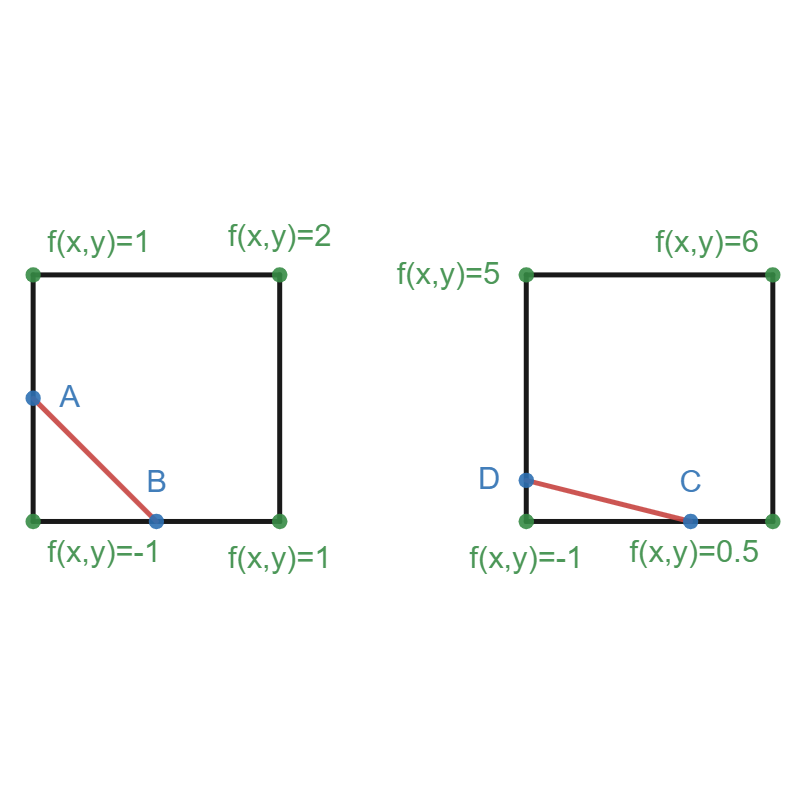
\includegraphics[width=0.5\textwidth]{linear_interpolation.png}
  \label{fig:linear_interpolation}
\end{SCfigure}

\begin{figure}[H]
  \caption{2D example of Marching Cubes approximating a circle on a 6x6 grid.}
  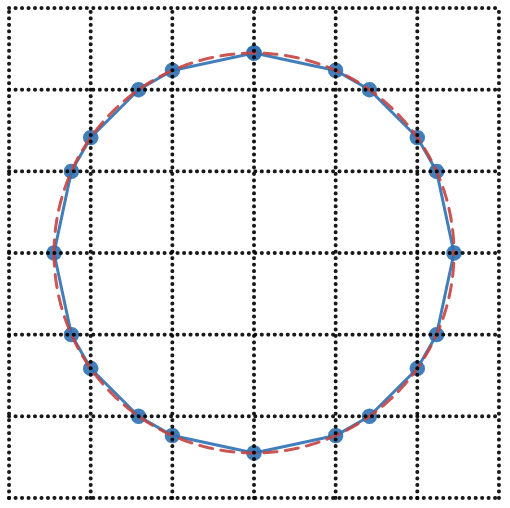
\includegraphics[width=0.7\textwidth]{ms_example.png}
  \label{fig:ms_example}
\end{figure}

\subsubsection{Limitations of Marching Cubes}
Marching Cubes was chosen for this project because the geometry for each grid cell can be generated independently from other cells. It produces a relatively accurate result for smooth shapes. However, it is not the best choice of algorithm for shapes with sharp corners, such as the shape in figure \ref{fig:sharp_corner}.
\begin{figure}[H]
  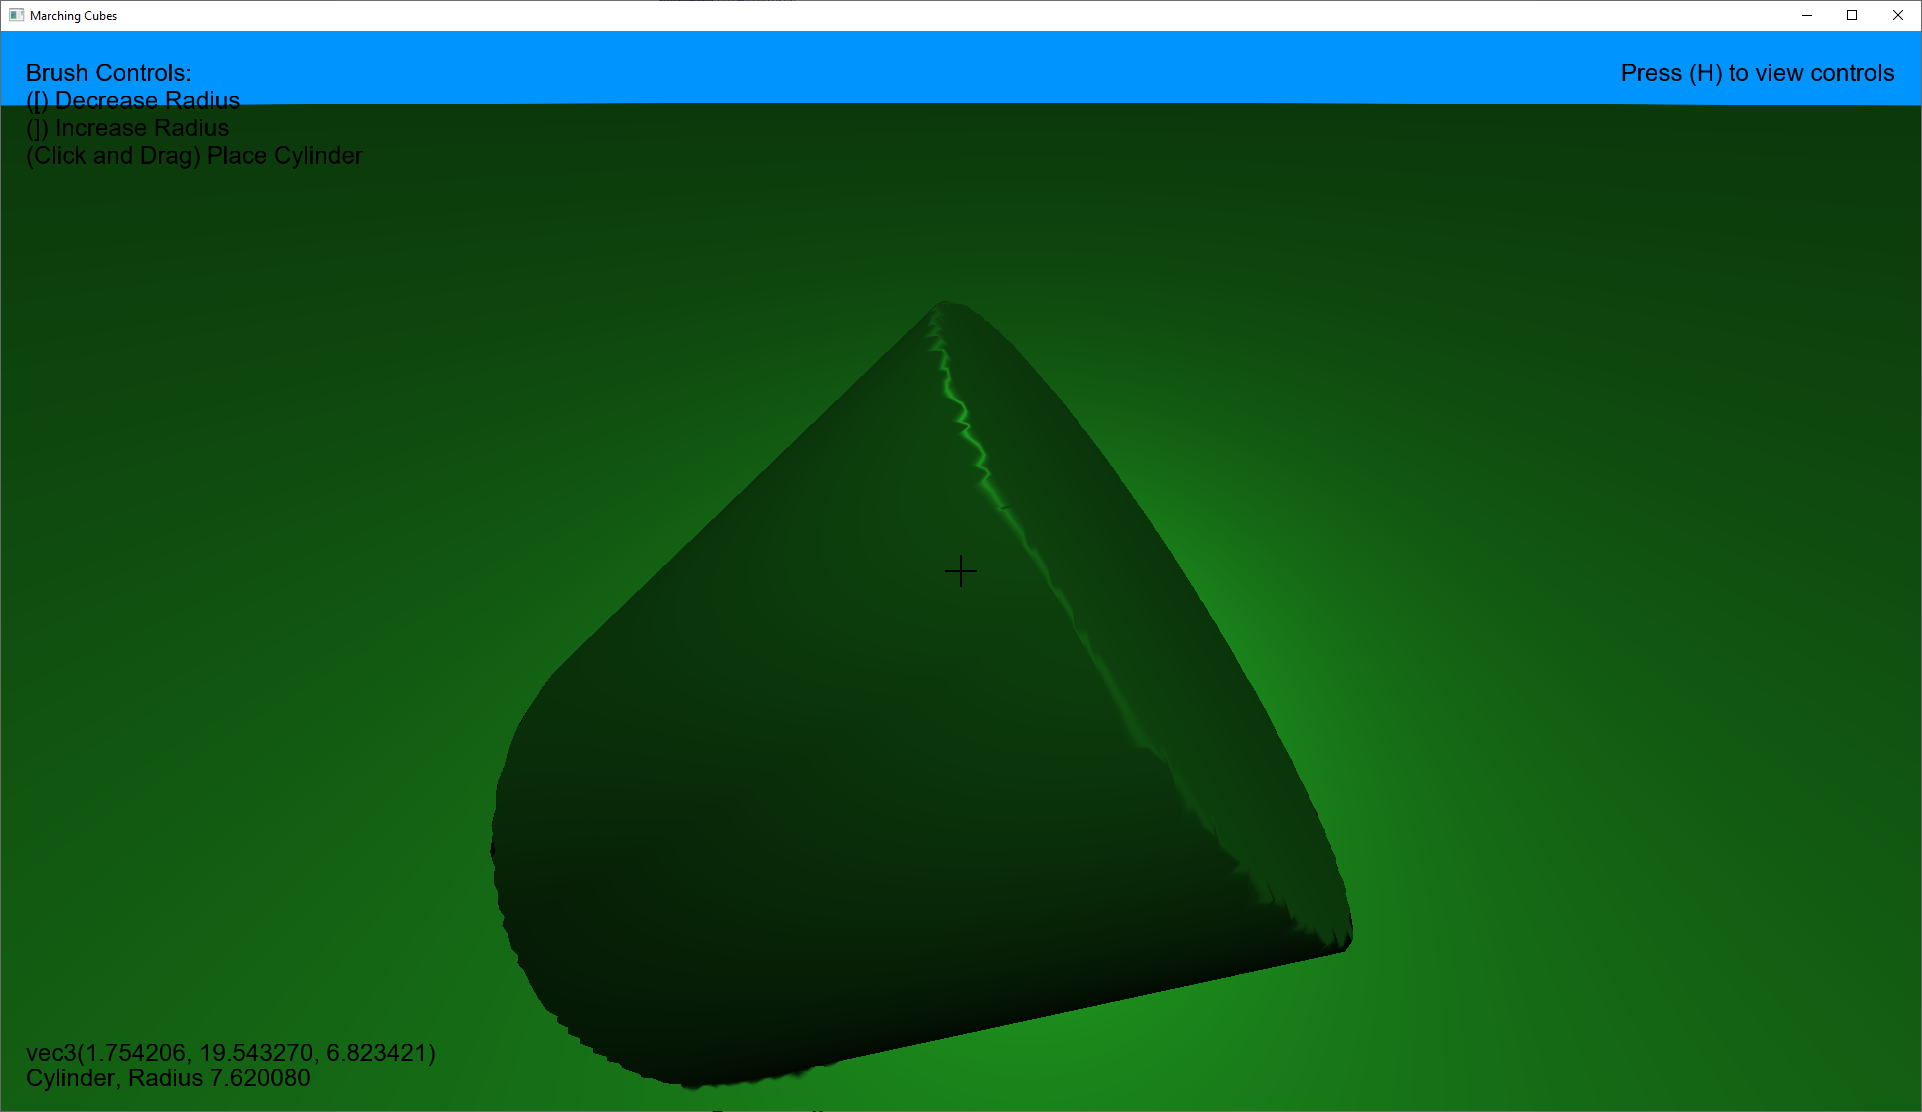
\includegraphics[width=\textwidth]{mc_cylinder.png}
  \caption{Inaccuracies near the sharp edge of this cylinder are visible.}
  \label{fig:sharp_corner}
\end{figure}
For this purpose, an algorithm such as Dual Contouring~\cite{10.1145/566654.566586} may produce better results. However, this algorithm generates triangles that span multiple grid cells, so it cannot be parallelised with the same method.

\subsection{GPU Programming} 
A GPU is designed for applications where a similar calculation is performed many times on varying data. Traditionally, this covers uses such as vertex shaders, which determine the position of every vertex in a 3D scene, or fragment shaders, which determine the color of every pixel on a screen. A modern GPU is capable of performing many millions of individual calculations per frame. In this project, we use the OpenGL API, and the C-style GLSL shader language that comes with it, to write code for the GPU.

We make use of compute shaders, which are not part of the graphics rendering pipeline, but are called by the OpenGL API and take advantage of the parallel architecture of the GPU. When a compute shader is executed, many invocations of the same code are executed in parallel, through the API function \texttt{glDispatchCompute}. These are indexed by the built-in GLSL variable \texttt{gl\_GlobalInvocationID}, a 3-component integer vector, that is different for each invocation. For example, a shader designed to calculate $f\left(x,y,z\right)$, for $ \left(x,y,z\right)$ ranging over integer-valued triples in $\left[0,32\right]^3$ would need to be configured so that \texttt{gl\_GlobalInvocationID} varies over all of the triples in this range.

To display geometry, and to interact with OpenGL, we make use of some open source libraries, namely GLFW~\cite{glfw}, for creating a window and handling input, GLEW~\cite{glew}, to load the OpenGL API functions, and GLM~\cite{g-truc_2005}, to provide mathematical functions such as manipulation of vectors, in C++.


\section{Algorithm Design}

\subsection{LOD System}
Even with an efficient GPU-based implementation, it becomes infeasible to generate and render a large uniform grid of Marching Cubes chunks. Generating large amounts of triangles far from the camera is unnecessary, since the detail will not be visible. For this reason, it is necessary to have a dynamic level of detail (LOD) system.

\subsubsection{Octree}
\label{section:octree}
To implement a versatile LOD system, an octree data structure is used. Each octree node represents a cuboid of space, such that the root node of the octree represents the entire renderable world, and the 8 children of an octree node equally divide the space represented by the parent node into octants. 

A \textit{chunk} refers to one of these regions of space, and consists of $n_x \cdot n_y \cdot n_z$ grid cells. The scale of these grid cells is determined by the depth of the octree node, with each level in the octree corresponding to a halving of the scale of a grid cell in each dimension. Geometry is generated at each leaf node, so the depth of the leaf node corresponds to the scale of the grid used within the generation algorithm, and hence the level of detail at which the geometry is generated. We will usually use chunks of size $32^3$, although other sizes are useful for demonstration purposes.

Using an octree, any condition can be used to determine the level of detail at any given point. We will use this in section \ref{section:physics_meshes} to control the level of detail around physics objects, for consistent collision detection. The level of detail is controlled with the functions \texttt{shouldSplit}, which returns whether a leaf node should split into its 8 children, and \texttt{shouldChop}, which returns whether a non-leaf node should become a leaf. When the octree changes, geometry associated with octree leaves that became branches, or were removed from the octree, is deleted, and new geometry is generated at each new leaf.

\begin{figure}[H]
  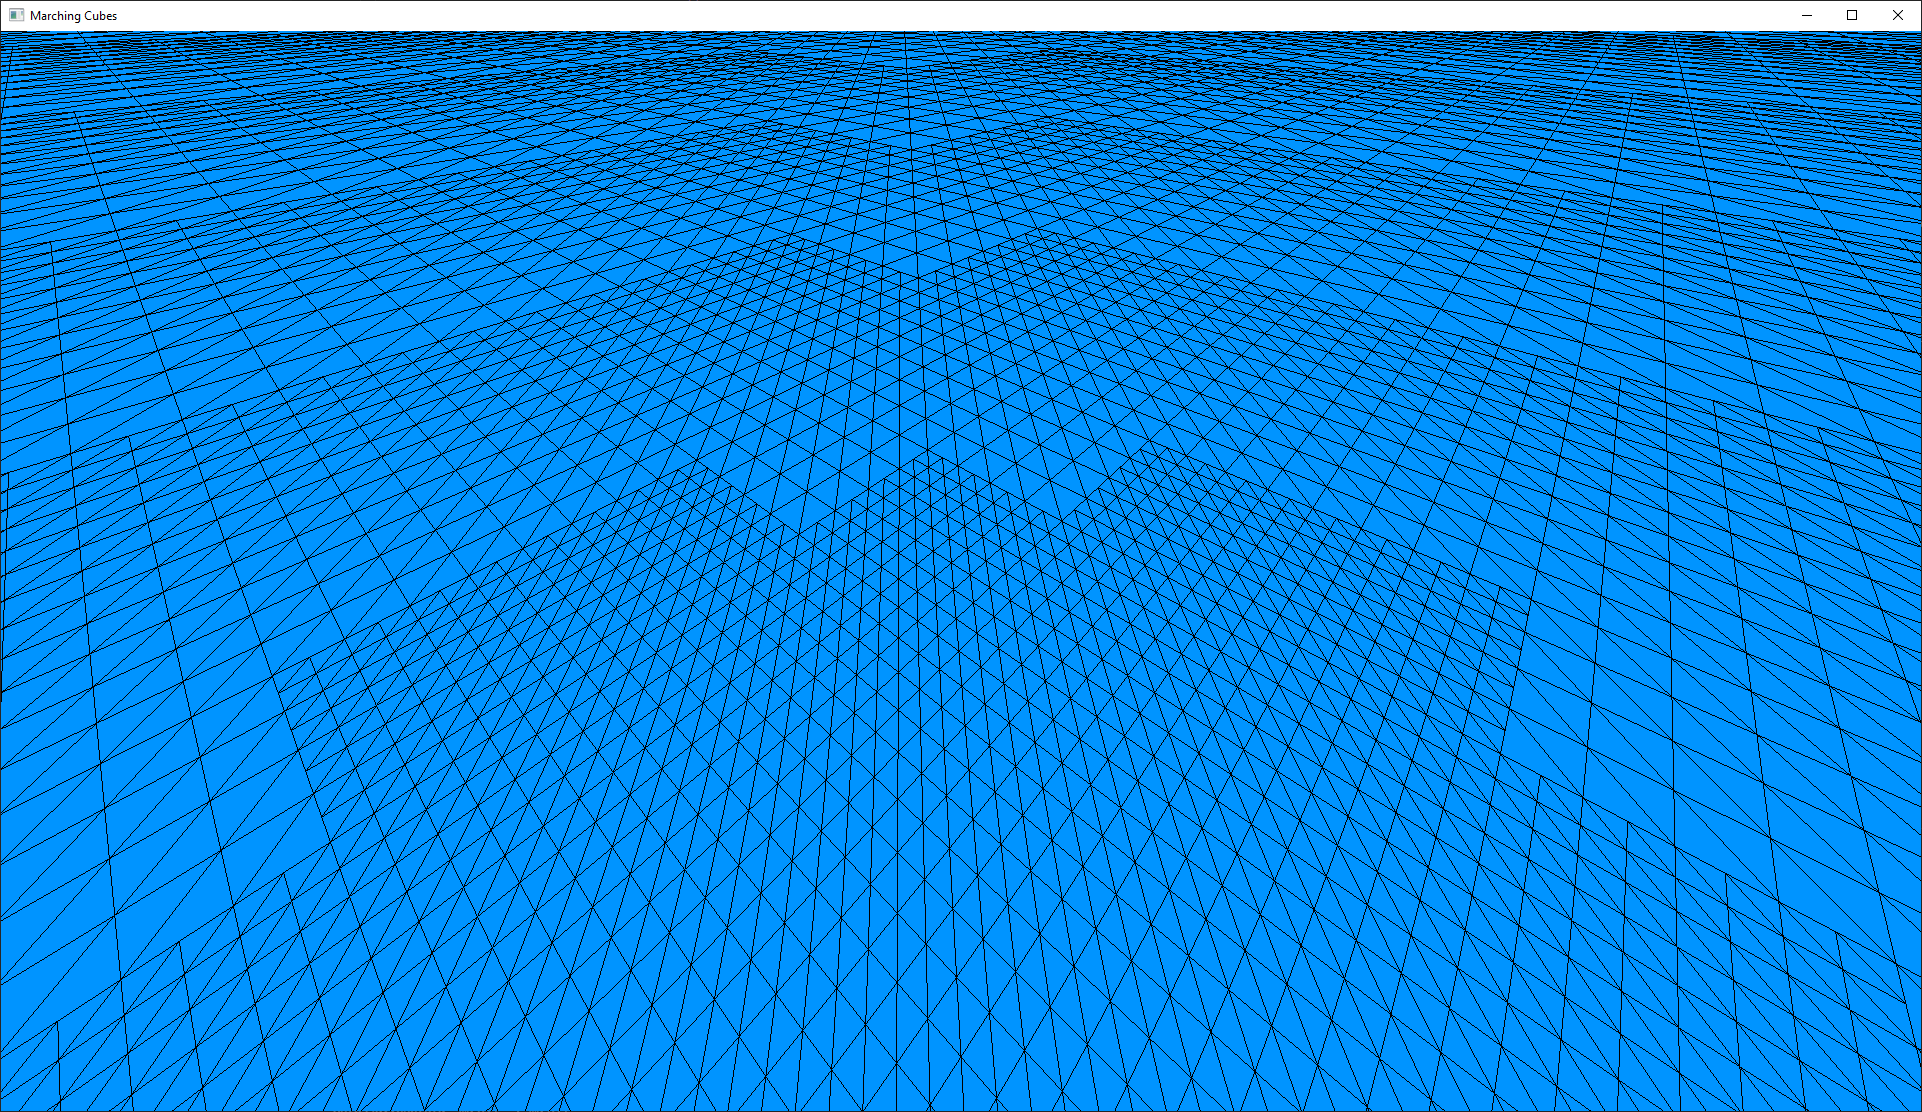
\includegraphics[width=\textwidth]{octree_plane.png}
  \caption{A plane generated using Marching Cubes, within this octree LOD system. Here, the chunk size is $4^3$. The level of detail is configured to decrease as the distance from the camera increases.}
\end{figure}

\subsection{The Transvoxel Algorithm}
\label{section:cracks}
Using Marching Cubes with multiple different grid cell sizes causes cracks on the boundary between chunks at different scales, since the vertices generated at different grid scales do not always line up with each other. Figure \ref{fig:cracks_demo} illustrates this, and figure \ref{fig:cracks2} shows the problem within my implementation.

\begin{SCfigure}[][!h]
  \caption{This figure shows the faces of 2 adjacent grid cells. The exact surface represented by the SDF is shaded in purple. The dotted lines show the edges produced by Marching Cubes at the level of detail of these grid cells, and the level below. When these cases occur next to each other, the red space in between the dotted lines forms a crack in the geometry.}
  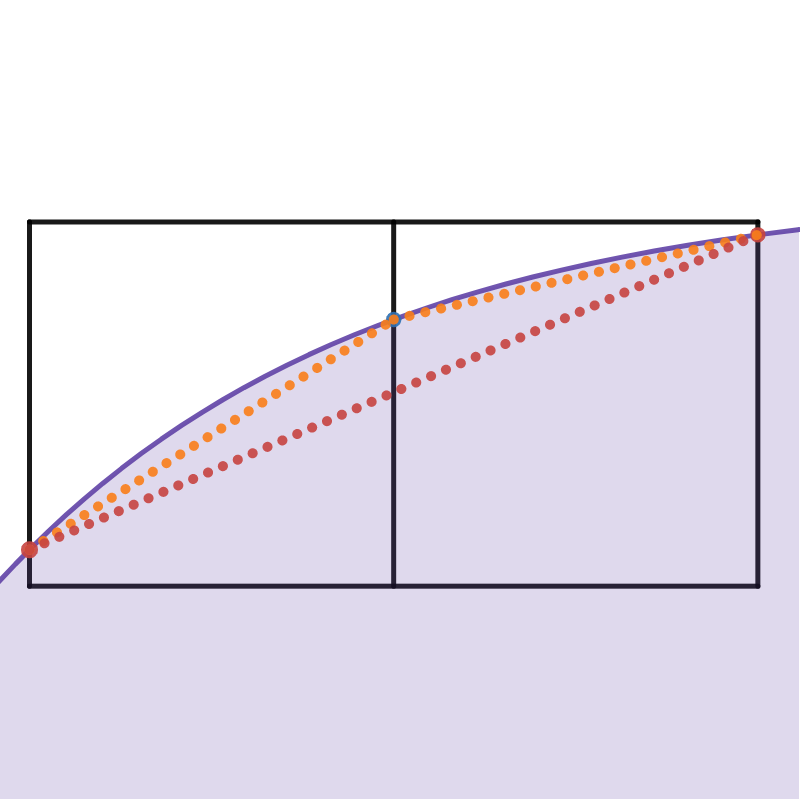
\includegraphics[width=0.5\textwidth]{cracks_demo.png}
  \label{fig:cracks_demo}
\end{SCfigure}

\begin{figure}[H]
  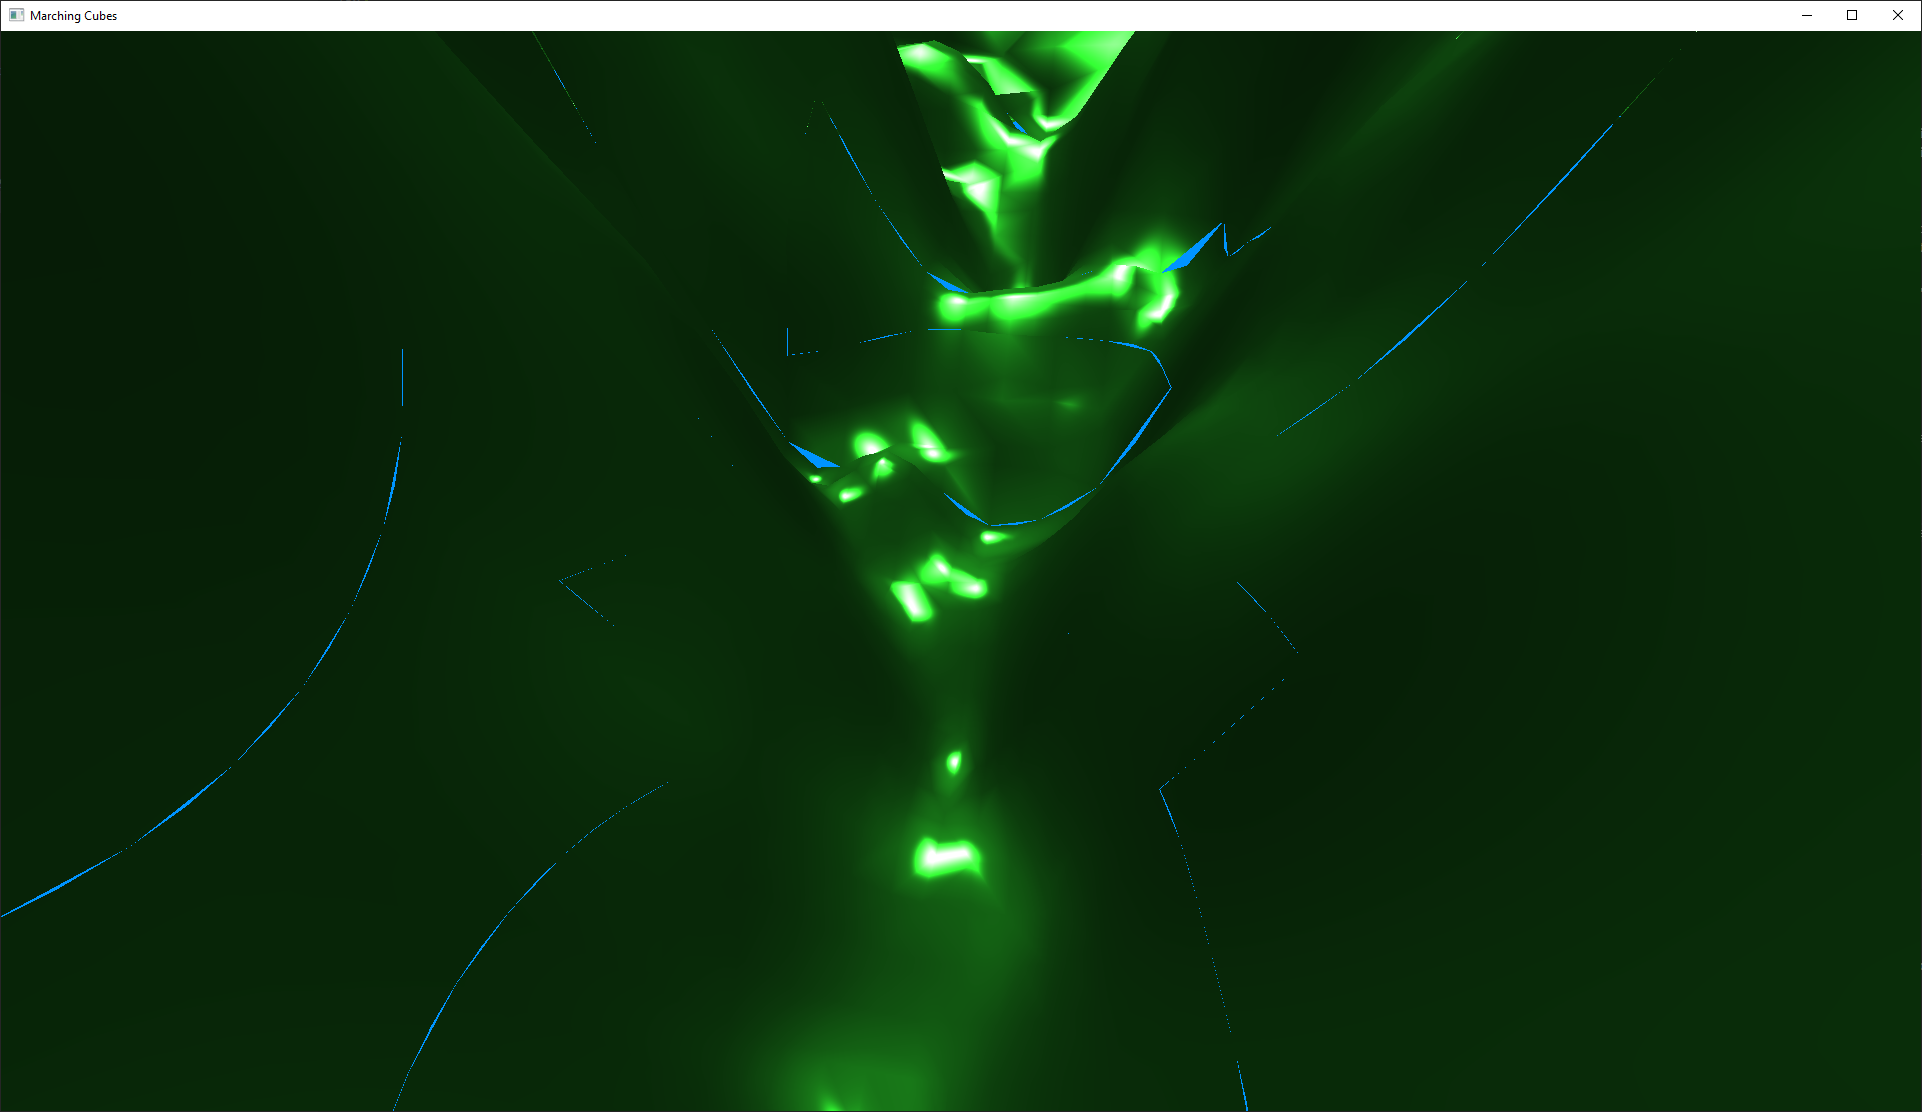
\includegraphics[width=\textwidth]{cracks2.png}
  \caption{Cracks between different levels of detail cause the blue background to be visible between chunks.}
  \label{fig:cracks2}
\end{figure}

The Transvoxel algorithm~\cite{lengyel_2010} is an algorithm based on Marching Cubes that solves this problem by adding additional vertices along cell edges that are adjacent to higher resolution grid cells.

This is done by splitting a cell at the lower resolution (a half-resolution cell) into a regular cell and some amount of transition cells, so that transition cells border the regular cells at the higher resolution (full-resolution cells). These transition cells serve as a method of stitching the gap in between half-resolution and full-resolution cells.
\begin{figure}[H]
  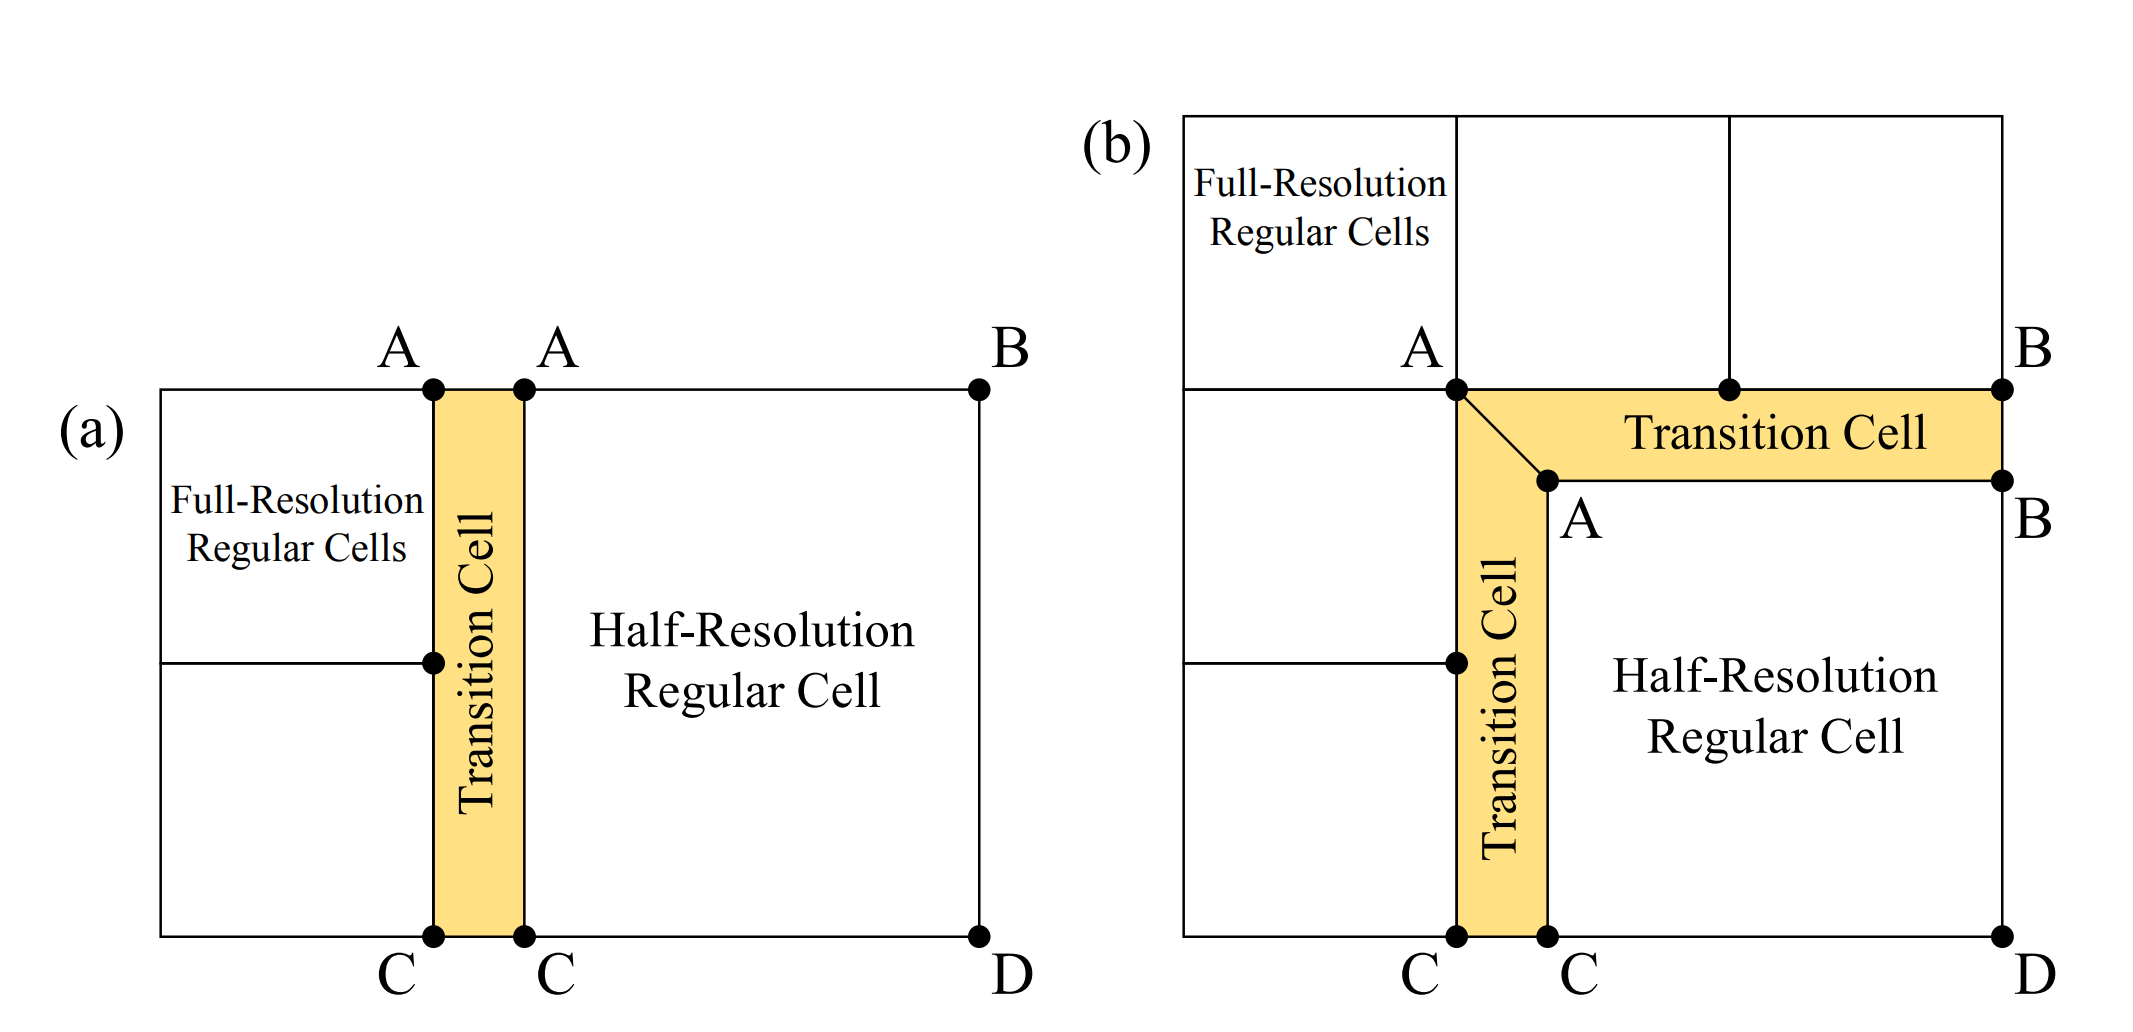
\includegraphics[width=\textwidth]{transition_cells}
  \caption{Illustration of 2 possible configurations of transition cells on the boundary between levels of detail. The half-resolution regular cell has been resized, and transition cells fit in the space made in between the cells. Reproduced from figure 4.9 in the Transvoxel algorithm paper~\cite{lengyel_2010}.}
  \label{fig:transition_cells}
\end{figure}

Like Marching Cubes, the original Transvoxel implementation was written for a standard CPU. It works similarly to Marching Cubes, relying on large lookup tables, and can be implemented to work independently on grid cells, so it is possible to take advantage of the parallel processing power of the GPU. We will modify a set of lookup tables provided by the original author of the Transvoxel algorithm~\cite{lengyel_2009}. A useful graphic showing all of the possible triangulations in the Transvoxel algorithm is available from the same source~\cite{lengyel}.

\subsubsection{Lookup Tables}
\label{section:lookup_tables}

This section demonstrates the functions of the Transvoxel lookup tables. These tables have been flattened from multidimensional arrays, since they will be passed to shaders as buffers. Vertex indexing data that would allow for reuse of vertices has been removed, for the reason described in section \ref{section:downsides}.

\paragraph{Regular cell lookup tables}
Regular cells have 8 cell vertices, each of which has a distinct SDF sample value. Figure \ref{fig:tv_labels} shows the vertex naming conventions for regular cells.

\begin{SCfigure}[][!h]
  \caption{Regular cell vertex naming convention. Reproduced from figure 3.7 of the Transvoxel paper~\cite{lengyel_2010}.}
  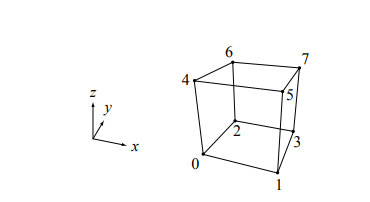
\includegraphics[width=0.5\textwidth]{tv_labels.PNG}
  \label{fig:tv_labels}
\end{SCfigure}

\begin{lstlisting}[language=C++,label={tv_tables},caption={Calculation of \texttt{cellIndex}, and lookup tables, for regular cells. An example of their usage is given below.}]
int cellIndex = 0;
int cellMask = 1;
for (int i = 0; i < 8; i++) {
  if (gridCells[i] < 0) cellIndex |= cellMask;
  cellMask = cellMask << 1;
}

const unsigned int regularCellClass[256] =
{
  0x00, 0x01, 0x01, 0x03, 0x01, 0x03, 0x02, 0x04, 0x01, 0x02, 0x03, 0x04, 0x03, 0x04, 0x04, 0x03,
  ...
};

const unsigned int regularCellData[256] =
{
  0x00, 0,0xFF,0xFF,0xFF,0xFF,0xFF,0xFF,0xFF,0xFF,0xFF,0xFF,0xFF,0xFF,0xFF,0xFF,
  0x31, 0, 1, 2,0xFF,0xFF,0xFF,0xFF,0xFF,0xFF,0xFF,0xFF,0xFF,0xFF,0xFF,0xFF,
  ...
};

const unsigned int regularVertexData[3072] =
{
  0xFF, 0xFF, 0xFF, 0xFF, 0xFF, 0xFF, 0xFF, 0xFF, 0xFF, 0xFF, 0xFF, 0xFF,
  0x01, 0x02, 0x04, 0xFF, 0xFF, 0xFF, 0xFF, 0xFF, 0xFF, 0xFF, 0xFF, 0xFF,
  ...
};

const unsigned int regularTotalTable[16] = {
  0,
  3,
  ...
};
\end{lstlisting}

The array \texttt{gridCells} contains the SDF sample values, and \texttt{cellIndex} is an index into the subsequent tables, calculated based on these values. 
\texttt{regularCellClass} maps the 256 possible values of \texttt{cellIndex} to one of 16 cell classes, which defines the triangulation used within the cell. There are actually 18 possible classes, however some of them use the same triangulation with different vertices, and this information is stored in \texttt{regularCellData}, so only 16 classes need to be considered. 
\texttt{regularCellData} contains a row of 16 numbers for each of the 16 cell classes. Each row starts with a value that encodes the number of distinct vertices and triangles in the triangulation, which is unused in my implementation. The following 15 entries are indices into \texttt{regularVertexData}, storing the order in which the vertices in the cell triangulation will be used. 
\texttt{regularVertexData} contains a row of 12 numbers for each \texttt{cellIndex}. Each number encodes an edge of the grid cell using 2 vertex indices, as in figure \ref{fig:tv_labels}. 
Finally, \texttt{regularTotalTable} contains the number of vertices in the triangulation for each class, including duplicates. This acts as a replacement for the unused triangle count in \texttt{regularCellData}.
As an example, consider the case where only vertex 0 is inside the terrain, giving a binary \texttt{cellIndex} of $00000001$. This will generate geometry like figure \ref{fig:regular_cell_example_case}. The cell class, from \texttt{regularCellClass}, is \texttt{0x01}. The number of vertices to be generated, from \texttt{regularTotalTable}, is 3. The vertex indices to be used, from \texttt{regularCellData}, are 0, 1, and 2. The vertex positions, from \texttt{regularVertexData}, are \texttt{0x01, 0x02, 0x04}. Hence a triangle will be generated with a vertex on the edge between grid cell vertices 0 and 1, a vertex on the edge between grid cell vertices 0 and 2, and a vertex on the edge between grid cell vertices 0 and 4, in that order.

\begin{SCfigure}[][!h]
  \caption{A regular cell of the same class as the example, reproduced from the diagram of all Transvoxel cell classes~\cite{lengyel}. Note however that this cell is not oriented the same as figure \ref{fig:tv_labels}.}
  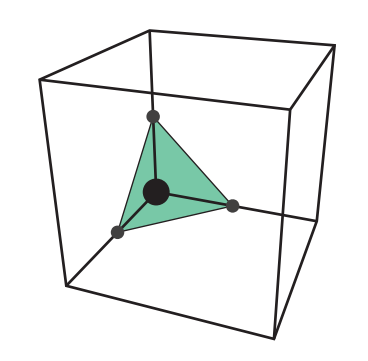
\includegraphics[width=0.5\textwidth]{regular_cell_example_case.PNG}
  \label{fig:regular_cell_example_case}
\end{SCfigure}

\paragraph{Transition cell lookup tables}

A transition cell uses 9 distinct SDF sample values, at vertices 0 through 8 in figure \ref{fig:tv_transition_labels}. Cell vertices 9, A, B, and C take their sample values from the vertices directly opposite them: vertices 0, 2, 6, and 8 respectively. Thus there are 512 possible cases to consider, rather than 256 cases in the case of a regular cell. Figure \ref{fig:tv_transition_cellIndex} shows how cell vertices are considered, for the purpose of calculating \texttt{transitionCellIndex}, as implemented in listing \ref{tv_transition_tables}.

\begin{SCfigure}[][!h]
  \caption{Cell vertex naming convention for transition cells. (a) shows the higher resolution face of the cell, and (b) shows the opposite, lower resolution face. Reproduced from figure 4.16 of the Transvoxel paper~\cite{lengyel_2010}.}
  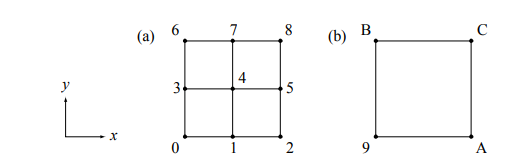
\includegraphics[width=0.5\textwidth]{tv_transition_labels.PNG}
  \label{fig:tv_transition_labels}
\end{SCfigure}

\begin{SCfigure}[][!h]
  \caption{Hexadecimal contribution to \texttt{transitionCellIndex} by each cell vertex on the higher resolution face of a transition cell. Reproduced from figure 4.17 of the Transvoxel paper~\cite{lengyel_2010}.}
  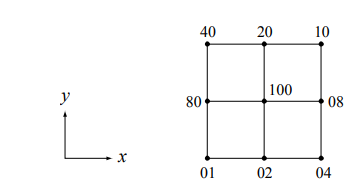
\includegraphics[width=0.5\textwidth]{tv_transition_cellIndex.PNG}
  \label{fig:tv_transition_cellIndex}
\end{SCfigure}



\begin{lstlisting}[language=C++, label={tv_transition_tables}, caption={Calculation of \texttt{transitionCellIndex}, and lookup tables for transition cells. An example of their usage is given below.}]
//Note the obscure order of this - see Figure 4.17 in transvoxel paper
//order is 0,1,2,5,8,7,6,3,4
int transitionCellIndex = 0;
int transitionFaceOrder[9] = int[](0,1,2,5,8,7,6,3,4);
int transitionCellMask = 1;
for (int i = 0; i < 9; i++) {
  if (transitionGridCells[transitionFaceOrder[i]] < 0) transitionCellIndex |= transitionCellMask;
  transitionCellMask = transitionCellMask << 1;
}

const unsigned int transitionCellClass[512] =
{
  0x00, 0x01, 0x02, 0x84, 0x01, 0x05, 0x04, 0x04, 0x02, 0x87, 0x09, 0x8C, 0x84, 0x0B, 0x05, 0x05,
  ...
};

const unsigned int transitionCellData[2072] =
{
  0x00, 0xFF,0xFF,0xFF,0xFF,0xFF,0xFF,0xFF,0xFF,0xFF,0xFF,0xFF,0xFF,0xFF,0xFF,0xFF,0xFF,0xFF,0xFF,0xFF,0xFF,0xFF,0xFF,0xFF,0xFF,0xFF,0xFF,0xFF,0xFF,0xFF,0xFF,0xFF,0xFF,0xFF,0xFF,0xFF,0xFF,
  0x42, 0, 1, 3, 1, 2, 3,0xFF,0xFF,0xFF,0xFF,0xFF,0xFF,0xFF,0xFF,0xFF,0xFF,0xFF,0xFF,0xFF,0xFF,0xFF,0xFF,0xFF,0xFF,0xFF,0xFF,0xFF,0xFF,0xFF,0xFF,0xFF,0xFF,0xFF,0xFF,0xFF,0xFF,
  ...
};

const unsigned int transitionVertexData[6144] =
{
  0xFF, 0xFF, 0xFF, 0xFF, 0xFF, 0xFF, 0xFF, 0xFF, 0xFF, 0xFF, 0xFF, 0xFF,
  0x01, 0x03, 0x9B, 0x9A, 0xFF, 0xFF, 0xFF, 0xFF, 0xFF, 0xFF, 0xFF, 0xFF,
  ...
};

const unsigned int transitionTotalTable[56] = {
  0,
  6,
  ...
};       
\end{lstlisting}

The tables perform the same roles as their regular cell counterparts. There are 73 classes of transition cell, although by considering classes using the same triangulation with different vertices, this can be reduced to 56 classes. The highest bit in the 8-bit \texttt{transitionCellClass} corresponds to a triangulation where the triangles face in the opposite direction, so a value of \texttt{0x87} in \texttt{transitionCellClass}, having binary value $10000111$, corresponds to cell class \texttt{0x07}, with the triangles facing in the opposite direction. 
For example, consider the transition cell where vertex 0 is inside the terrain. Then vertex 9 will also be considered as inside. This will generate geometry like figure \ref{fig:transition_cell_example_case}. \texttt{transitionCellIndex} will be calculated as $000000001$, corresponding to a cell class of \texttt{0x01} in \texttt{transitionCellClass}. 
The number of vertices to generate is found in \texttt{transitionTotalTable}; in this case, there are 6. The vertex indices to be used are found in \texttt{transitionCellData}: The first triangle uses vertex indices 0, 1, and 3, in that order, and the second uses vertices 1, 2, and 3.
The locations of these vertices are found in the corresponding row in \texttt{transitionVertexData}, so vertex 0 is between cell vertices 0 and 1, vertex 1 is between cell vertices 0 and 3, and so on.

\begin{SCfigure}[][!h]
  \caption{A transition cell of the same class as the example, reproduced from the diagram of all Transvoxel cell classes~\cite{lengyel}.}
  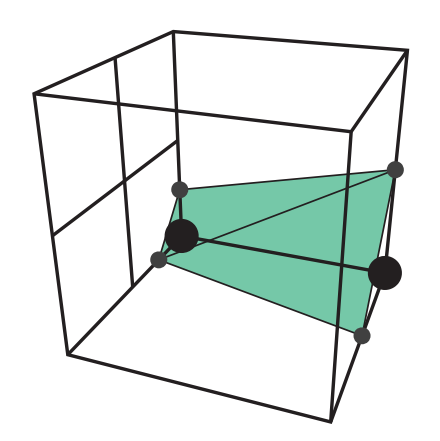
\includegraphics[width=0.5\textwidth]{transition_cell_example_case.PNG}
  \label{fig:transition_cell_example_case}
\end{SCfigure}

\subsubsection{Adaptation of the algorithm to GPU}

We now describe a Transvoxel implementation on the GPU, making use of these modified lookup tables. The algorithm is implemented in 3 separate compute shader phases, executed in order, to generate the geometry for a single chunk.

The chunk faces where transition cells should be generated are encoded in the variable \texttt{edgeIndex}, which is discussed in section \ref{section:edgeIndex}.

\begin{enumerate}
\item \underline{Distance function computation}: For each grid cell vertex, the SDF is sampled, and stored in a buffer. If this vertex lies on the face of the chunk, the SDF is sampled at additional points on the face, for use in transition cells. This shader is invoked once for each grid cell vertex, and the invocations corresponding to the vertices on the faces where transition cells are generated are responsible for calculating the additional sample points. This is done separately to the following stages to avoid unnecessary recomputation of the SDF, since one grid cell vertex may belong to up to 8 neighboring grid cells.

\begin{lstlisting}[language=C++,label={tv_generate},caption={Code snippet that samples the SDF at the grid point, as well as at the points needed for any transition cells on the -X and +X facing faces. The \texttt{generate} function is responsible for sampling the SDF and storing the value in a buffer, and takes 2 parameters: the first is the actual position of the grid cell vertex, and the second is an offset parameter, for generating sample values halfway beetween grid vertices. For example, a value of \texttt{uvec3(0,1,0)} corresponds to a point that is offset from the position in the first argument by half a grid cell in the Y direction.}]

void generate(uvec3 gid, uvec3 halfXYZ) {
  uint arrID = getArrID(gid, halfXYZ); //get index into buffer
  float value = modified_distance((gid + 0.5 * vec3(halfXYZ)) * chunkStride + chunkPosition); //compute the SDF
  distanceValues[arrID] = value;
}
void main() {
  uvec3 gid = gl_GlobalInvocationID;
  if (gid.x > chunkSize.x || gid.y > chunkSize.y || gid.z > chunkSize.z) {
    return;
  }
  generate(gid,uvec3(0)); //calculate the SDF at this grid point

  if ((gid.x == 0 && (edgeIndex & 1) != 0) || (gid.x == chunkSize.x && (edgeIndex & 2) != 0)) {
    if (gid.y < chunkSize.y) {
      generate(gid,uvec3(0,1,0)); //calculate the SDF at this grid point, offset by half the grid width in the y direction
    }
    if (gid.z < chunkSize.z) {
      generate(gid,uvec3(0,0,1));
    }
    if (gid.y < chunkSize.y && gid.z < chunkSize.z) {
      generate(gid,uvec3(0,1,1));
    }
  }
  ... //do the same for the y and z oriented faces  
}
\end{lstlisting}

\begin{SCfigure}[][!h]
  \caption{Illustration of the points to be sampled on the face of a 2x2x2 chunk when transition cells will be generated. The 4 blue points in the bottom left are those that will be sampled by an invocation on the vertex at $\left(0,0\right)$, the 2 green points in the bottom right will be sampled by an invocation on the vertex at $\left(2,0\right)$, and the singular purple point will be sampled by an invocation on the vertex at $\left(2,2\right)$.}
  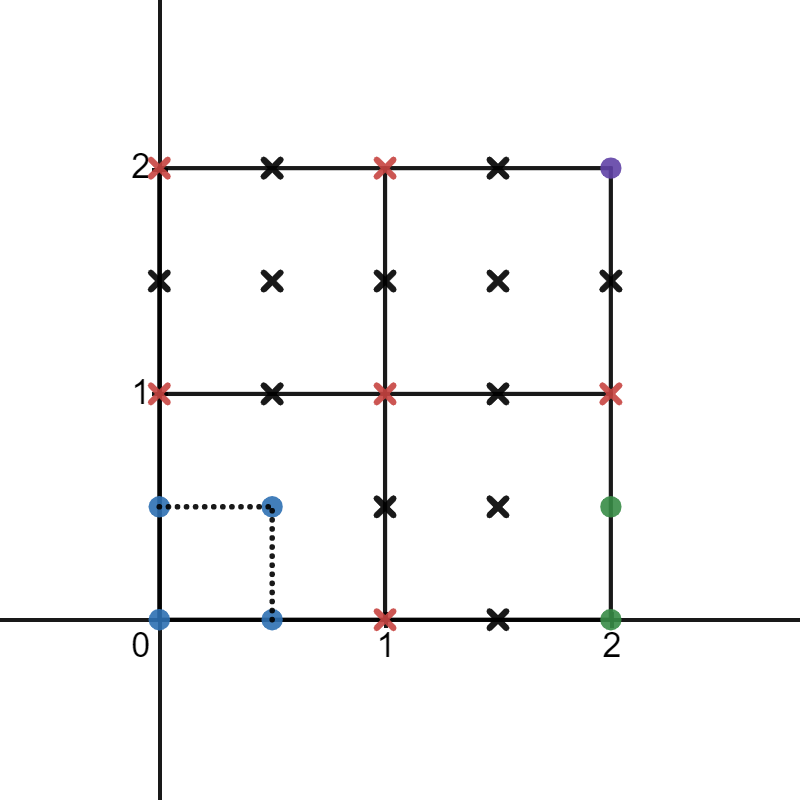
\includegraphics[width=0.5\textwidth]{tv_gen_grid}
  \label{fig:tv_gen_grid}
\end{SCfigure}

\item \underline{Counting phase}: For each regular cell, calculate the number of mesh triangles within it, and if this number is non-zero (the cell is not all air, or all solid), add it to the list of cells to generate geometry for in the next phase. 

\begin{lstlisting}[language=C++,label={tv_count_regular},caption={Code for counting the number of vertices and marchable grid cells in the chunk. Variable \texttt{cellIndex} is calculated according to listing \ref{tv_transition_tables}, using the SDF values from the previous stage.}]
if (cellIndex != 0 && cellIndex != 255) { //cell is not completely solid or air
  //record number of points in mesh
  atomicCounterAddARB(pointCount,regularTotalTable[regularCellClass[cellIndex]]);
  //get index into buffer to pass to next stage
  uint bufferIndex = atomicCounterIncrement(marchableCount);
  uvec4 mc = uvec4(gid.x,gid.y,gid.z,cellIndex);
  //store cell position and index in buffer
  marchableList[bufferIndex] = mc;
}
\end{lstlisting}
To handle transition cells, the following is done, for each possible orientation of transition cell:
\begin{itemize}
  \item Check whether a transition cell should be generated, based on \texttt{edgeIndex}, and whether this grid cell lies on the face of the chunk. If not, then skip the rest of the generation.
  \item Determine the values of the SDF on the higher resolution face of the transition cell, using the buffer passed from the previous phase. Use this information to calculate the variable \texttt{transitionCellIndex}.
  \item Use the lookup tables to determine how much geometry exists within this transition cell, and increase the atomic counter accordingly.
  \item Append this transition cell to the buffer of cells to be polygonised in the subsequent phase. It will be polygonised separately from the regular cell that exists within the same grid cell.
\end{itemize}

\begin{lstlisting}[language=C++,label={tv_count},caption={Part of the code responsible for counting the triangles in transition cells, and appending them to the geometry generation buffer. The first 9 bits of \texttt{paddedTransitionCellIndex} store the value of \texttt{transitionCellIndex}, calculated as shown in figure \ref{fig:tv_transition_cellIndex}. Bit 10 records that the cell is a transition cell, and exactly one of bits 11-16 will be set, to store the orientation of the cell.}]
//cell is a transition cell:
int paddedTransitionCellIndex = transitionCellIndex;
paddedTransitionCellIndex |= (1<<9);

//store cell orientation:
paddedTransitionCellIndex |= (mask<<10);

//do not march if all inside or all outside
if (transitionCellIndex != 0 && transitionCellIndex != 511) {
  //number of points in the mesh
  //and with 0x7f for lookup table - handles case where opposite facing triangles are used
  atomicCounterAddARB(pointCount,transitionTotalTable[0x7F & transitionCellClass[transitionCellIndex]]);

  uint bufferIndex = atomicCounterIncrement(marchableCount);
  //store grid position in the first 3 coordinates, cell index and orientation padded into single int in the 4th coordinate
  uvec4 mc = uvec4(gid.x,gid.y,gid.z,paddedTransitionCellIndex);
  marchableList[bufferIndex] = mc;
}
\end{lstlisting}

\item \underline{Polygonisation phase}: For each cell passed by the previous phase through the buffer \texttt{marchableList}, the geometry is created, and the vertices of the geometry are linearly interpolated as described in section \ref{section:mc}. 

\begin{lstlisting}[language=C++,label={tv_poly_regular},caption={Code for generating the geometry in a regular cell.}]
void generateCell() {
  //grid position in chunk
  uvec3 gid = marchableList[gl_GlobalInvocationID.x].xyz;

  float gridCells[8];
  ivec3 gridPos[8];

  //assigned as per Figure 3.7 in transvoxel paper - note this is DIFFERENT to the previous marching cubes algorithm
  for (int i = 0; i < 8; i++) {
    gridPos[i] = ivec3(gid) + gridOffset[i];
  }

  //transitionGridPos is the grid positions including the offset from the transition cells
  vec3 transitionGridPos[8];

  //hasShifted is true if the vertex has been moved as a result of being on a transition cell
  bool hasShifted[8];

  //calculate where the vertex actually is, based on which transition cells will be generated
  for (int i = 0; i < 8; i++) {
    vec3 avp = actualVertexPosition(gridPos[i]);
    transitionGridPos[i] = avp;
    hasShifted[i] = (avp != vec3(gridPos[i]));
  }

  //Actual distance values
  for (int i = 0; i < 8; i++) {
    gridCells[i] = distanceValues[getArrID(gridPos[i],uvec3(0))];
  }

uint cellIndex = marchableList[gl_GlobalInvocationID.x].w & ((1<<9)-1);
uint cellClass = regularCellClass[cellIndex];
uint totalPoints = regularTotalTable[cellClass];

  uint index = 0;
  for (int i = 0; i < totalPoints; i++) {
    if (i % 3 == 0) {
      //atomically get index into vertex and normal arrays
      index = atomicCounterIncrement(triCount);
    }
    uint vertexIndex = index * 3 + (i % 3);

    //vertex positions
    uint vertexData = regularVertexData[cellIndex * 12 + regularCellData[cellClass * 16 + 1+i]];
    uint v1Index = vertexData & 0x0F;
    uint v2Index = vertexData >> 4;

    //linear interpolation
    vec3 vertPos = VertexInterp(transitionGridPos[v1Index],transitionGridPos[v2Index],gridCells[v1Index],gridCells[v2Index]);

    if (hasShifted[v1Index] || hasShifted[v2Index]) { //if this vertex has moved
      //apply the transformation as in Figure 4.12 in the Transvoxel paper
      //where the vertex would have been
      vec3 vp2 = VertexInterp(gridPos[v1Index],gridPos[v2Index],gridCells[v1Index], gridCells[v2Index]);
      //normal at this position - in world space
      vec3 n = modified_normal(vp2 * chunkStride + chunkPosition);
      vec3 dv = vertPos - vp2;
      vertPos -= (dot(n,dv)) * n;
    }

    //convert to world coordinates
    vertPos = vertPos * chunkStride + chunkPosition;

    //store vertex and normal
    vertices[vertexIndex] = vec4(vertPos,1);
    normals[vertexIndex] = vec4(modified_normal(vertPos),0);
  }
}
\end{lstlisting}
When a regular cell has been made smaller to accommodate transition cells, the SDF has been sampled at the grid cell vertices, rather than the vertices of the regular cell. This introduces inaccuracies in the resulting geometry. The Transvoxel algorithm paper describes a transformation that solves this issue by moving vertices on the lower resolution face of the transition cell, and the corresponding vertex on the neighboring regular cell, so they are on the edge that the regular cell would have generated. This was implemented in listing \ref{tv_poly_regular}.

Transition cells are handled separately from regular cells, even if they share the same grid cell. There are multiple possible shapes a transition cell may need to take, some of which were shown in figure \ref{fig:transition_cells}. The cell vertex positions are calculated based on \texttt{edgeIndex}. Since the presence of a transition cell means that a regular cell has been resized, the transformation described above is performed for all geometry generated on the lower resolution face of the transition cell. Otherwise, the actual code used to determine the geometry is similar, using the lookup tables from listing \ref{tv_transition_tables}.

There is a case where multiple vertices of a transition cell may be moved to the same place, resulting in zero-width triangles being generated, which could interfere with other algorithms the generated geometry is used with. However, the number of zero-width triangles is small, and it turns out that in the applications considered in this report, zero-width triangles have not caused any issues.

\begin{figure}[H]
  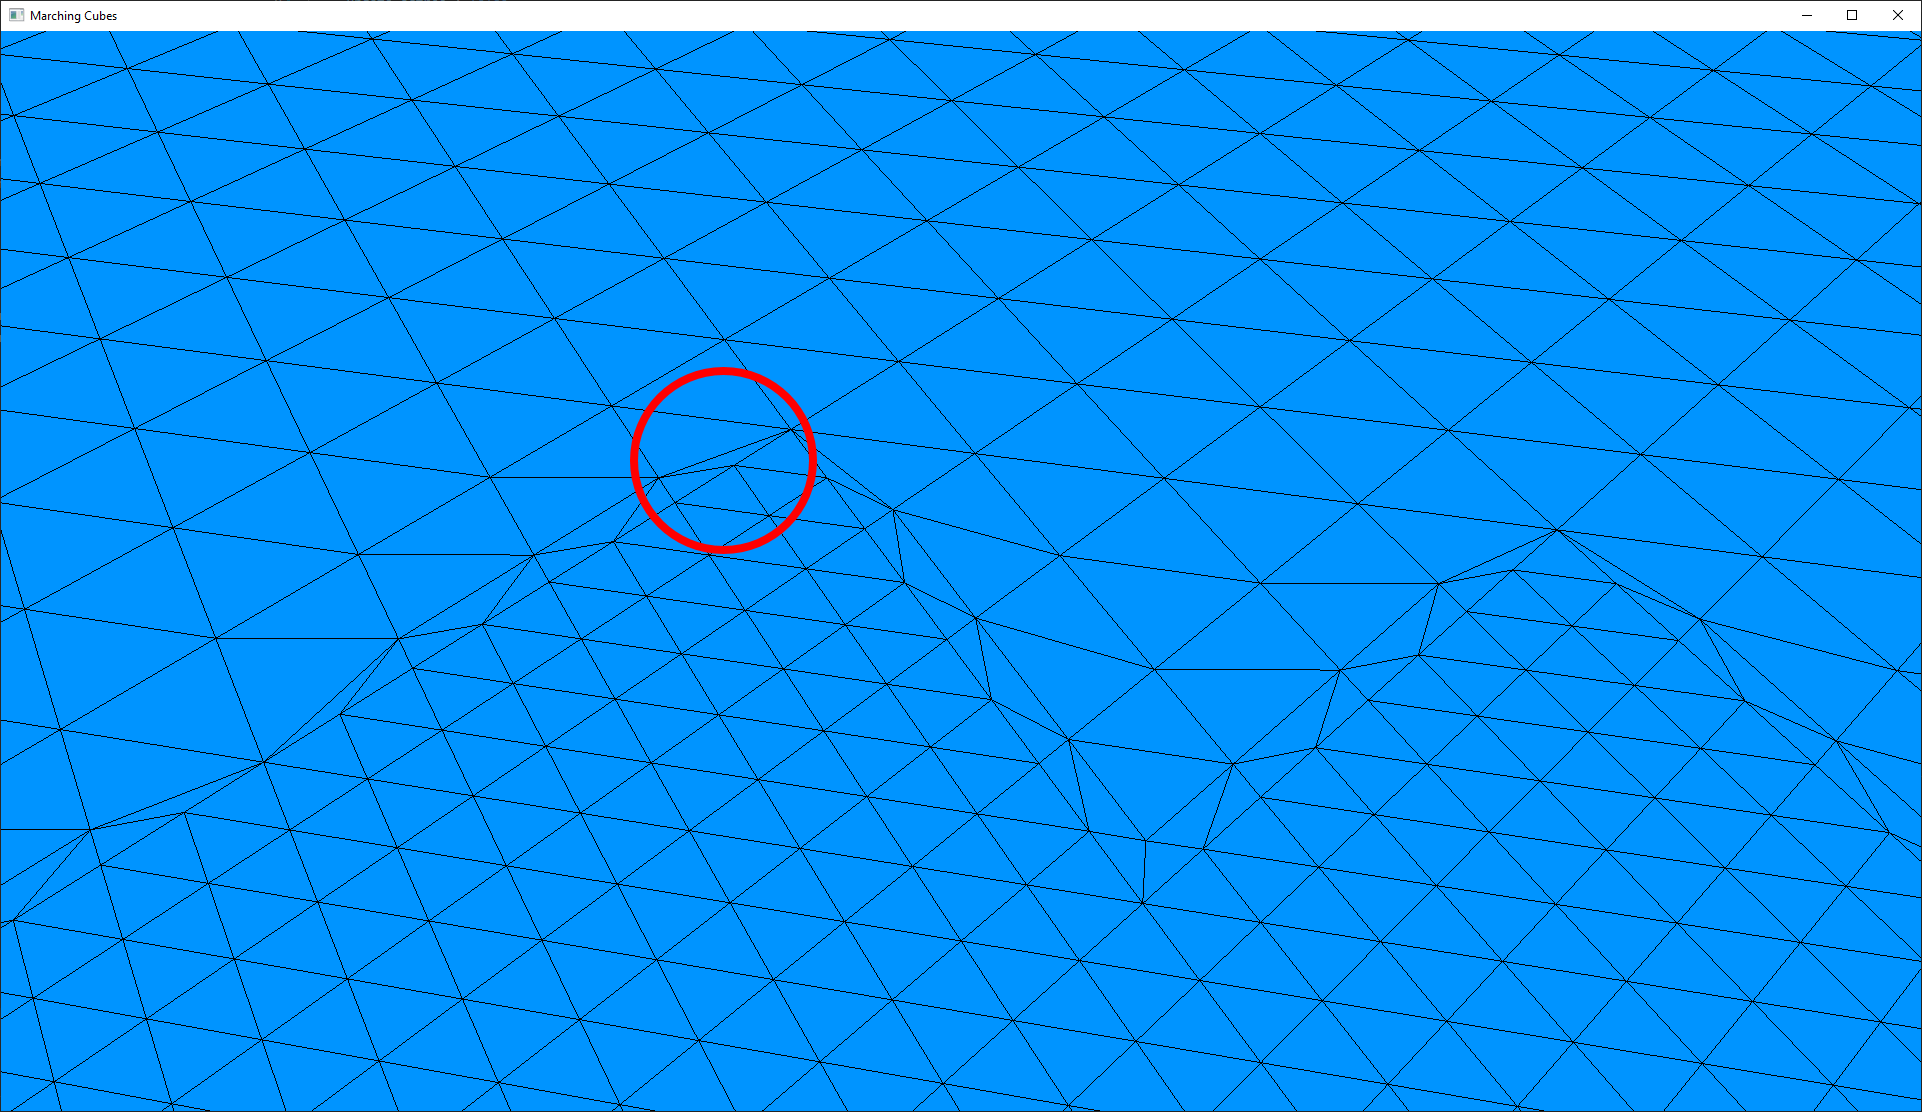
\includegraphics[width=\textwidth]{tv_transition_plane}
  \caption{A plane generated with the Transvoxel algorithm. The circled transition cell has vertices placed on top of each other, leading to zero-width triangles.}
  \label{fig:tv_transition_plane}
\end{figure}

\end{enumerate}

\subsubsection{Calculation of edgeIndex}
\label{section:edgeIndex}

The variable \texttt{edgeIndex} is a 6-bit integer, with each bit storing whether a face of a chunk should have transition cells. For each octree leaf containing geometry, the octree is searched using a recursive algorithm, to find neighboring nodes in each direction at the same depth. If a neighbor is a leaf, then the neighboring geometry is at the same level of detail. If no neighbor exists at the same depth in some direction, then the neighboring geometry is at a lower level of detail. \texttt{edgeIndex} is not modified in this case, since it will be modified for the lower level of detail geometry. If the neighbor is not a leaf, then the neighboring geometry is at a higher level of detail, and \texttt{edgeIndex} is modified to record that transition cells should be generated in that direction. Figure \ref{fig:octree_neighbors} shows some example cases.

\begin{SCfigure}[][!h]
  \caption{The blue cell has 3 neighbors at the same level of detail. The green neighbor is within the same parent octree cell, and no recursive calls are needed. The red neighbor is not within the same parent cell, so the neighbor of the parent is found, and the corresponding child of this neighbor is returned. The orange neighbor is not a leaf, so \texttt{edgeIndex} is updated to reflect this. There is no neighbor at the same level of detail above the blue cell.}
  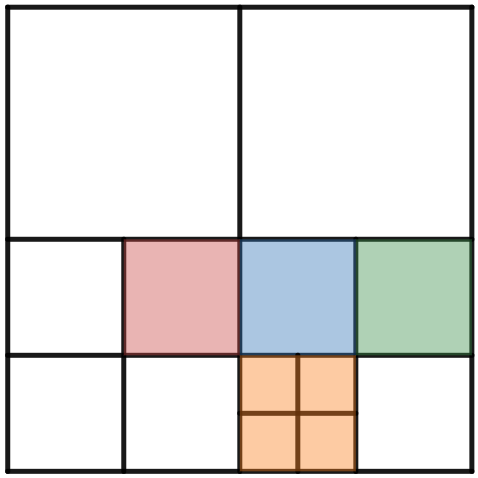
\includegraphics[width=0.5\textwidth]{octree_neighbors.png}
  \label{fig:octree_neighbors}
\end{SCfigure}

\begin{lstlisting}[language=C++,label={octree_neighbor},caption={Code for finding the neighbor of a node at the same level of detail in an octree. The children of a node are stored as a 3D array of pointers: \texttt{Octree* myChildren[2][2][2];}. \texttt{relativePosition} is a 3-component vector, where exactly one component is non-zero, corresponding to the direction in which to look for the neighbor. For example, a value of $\left(1,0,0\right)$ searches in the positive X direction.}]
//return the neighbor at the same LOD if one exists, or NULL if none exists
//whether this is a leaf or not determines the edge index
Octree* Octree::getNeighbor(glm::ivec3 relativePosition) {
  if (!myParent) {
    return NULL;
  }
  glm::ivec3 childPosition = relativePosition + glm::ivec3(myPositionInParent);
  if (glm::all(glm::greaterThanEqual(childPosition, glm::ivec3(0))) && glm::all(glm::lessThanEqual(childPosition,glm::ivec3(1)))) {
    //return the parent child at this relative position
    return myParent->childFromVec3(childPosition);
  } else {
    //return the child of the parent neighbor
    Octree* neighbor = myParent->getNeighbor(relativePosition);
    if (!neighbor || neighbor->isLeaf) return NULL;
    //glm does not have integer mod, so we have to do this manually...
    glm::ivec3 childOppositePosition = glm::abs(glm::ivec3(childPosition.x % 2, childPosition.y % 2, childPosition.z % 2));
    return neighbor->childFromVec3(childOppositePosition);
  }
}
\end{lstlisting}


\subsubsection{Downsides of Parallelisation}
\label{section:downsides}
This method of parallelisation presents some downsides. Triangles are placed into the vertex buffer as parallel invocations of the third compute shader increment the atomic counter, which may be different between calls. This means that there is no way to reliably use an index buffer for vertices, which would be beneficial since multiple vertices are often generated in the same place, resulting in many duplicates in the vertex array. This is why vertex indexing data was removed from the Transvoxel tables. Nevertheless, this is a worthwhile tradeoff, with the GPU implementation greatly outperforming the CPU implementation, as demonstrated in section \ref{section:GPUCPUcomparison}.



\subsubsection{Algorithm Speed Comparison}
\label{section:GPUCPUcomparison}
We now evaluate the performance of the parallel Transvoxel implementation, against a CPU implementation of Marching Cubes based on one by Paul Bourke~\cite{bourke_1994}, as well as an implementation of the same Marching Cubes algorithm, parallelised using the same 3-phase technique.

The SDF used for these comparison tests is a scaled 3D fractal noise function, as described in section \ref{section:noise}. An effort has been made to ensure the SDF is the same on the CPU and GPU, however due to floating point inaccuracies and differences between the GLSL and C++ implementations, the SDF occasionally produces slightly different values between implementations, and this results in the number of triangles generated being different. However, this difference is small compared to the total number of triangles generated, so is unlikely to have an impact on the runtime comparison.

Table \ref{tab:comparison-time} shows the time taken to generate different numbers of chunks of 3D noise, of size $32^3$, using each of the implementations described. When using the Transvoxel algorithm, transition cells have been generated on the +x, +y, and +z faces. This means that the number of triangles generated is also higher for the Transvoxel algorithm. Table \ref{tab:comparison-tris} shows the number of triangles generated in each experiment. All experiments were run using an Intel i9-9900k and Nvidia RTX 2080ti. Each experiment was run 5 times, and the average time is shown.
\begin{table}[H]
  \begin{tabular}{|c|c|c|c|}
    \hline
    Test & CPU Time (ms) & GPU Time (ms) & Transvoxel Time (ms)\\
    \hline
    \hline
    1 Chunk & 65.4 & 4.2 & 6.2\\
    4x4x4 Chunks &  6817.4 & 60.8 & 113.4\\
    10x1x10 Chunks & 12650.2 & 90.0 & 155.8\\
    10x10x10 Chunks & 117568.6 & 635.0 & 998.0\\
    \hline
    
  \end{tabular}
  \caption{\label{tab:comparison-time}Performance comparison between the 3 implementations.}
\end{table}


\begin{table}[H]
  \begin{tabular}{|c|c|c|c|}
    \hline
    Test & Marching Cubes (CPU) & Marching Cubes (GPU) & Transvoxel\\
    \hline
    \hline
    1 Chunk & 1054 & 1054 & 1054\\
    4x4x4 Chunks & 238981 & 238999 & 262377\\
    10x1x10 Chunks & 497911 & 497845 & 545848\\
    10x10x10 Chunks & 4394195 & 4394045 & 4816936\\
    \hline
  \end{tabular}
  \caption{\label{tab:comparison-tris}Difference in number of triangles generated between the 3 implementations. The number of triangles in the 1 chunk test is the same, even for the Transvoxel test, because no geometry is generated on the edge of the chunk.}
\end{table}



\begin{figure}[H]
  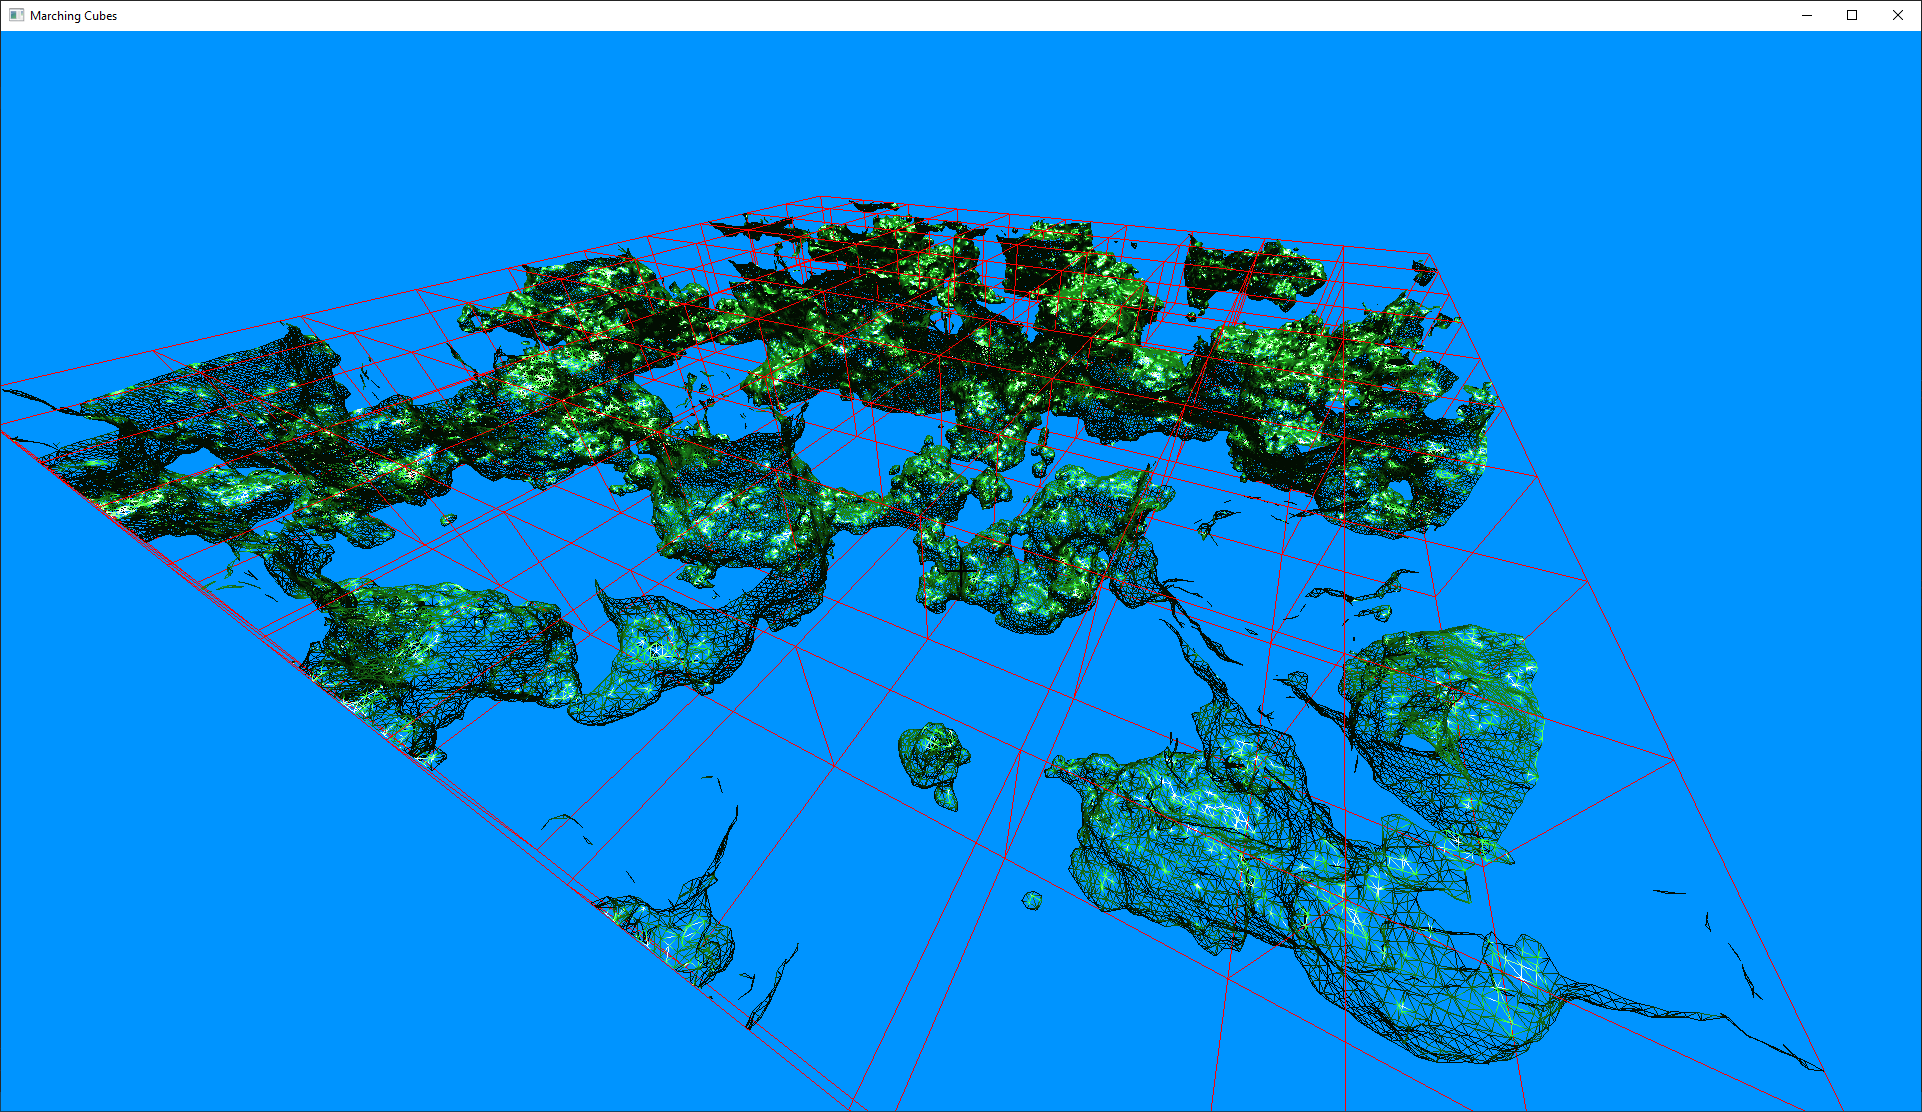
\includegraphics[width=\textwidth]{10x10_wireframe.png}
  \caption{A wireframe of the 10x1x10 chunk test.}
\end{figure}


\subsubsection{Octree Refinement}
\label{section:octree_refinement}
The Transvoxel algorithm is sufficient in most cases for eliminating cracks in the geometry. However, there are octree configurations which could occur, where different levels of detail appear next to each other, even once transition cells have been generated. Figure \ref{fig:octree_neighbor_error} shows an example of this.

\begin{SCfigure}[][!h]
  \caption{An illustration of where different levels of detail may occur next to each other. Areas where transition cells are generated are shaded in blue. The area where transition cells are generated, but different levels of detail will still be adjacent to each other, is shaded in red.}
  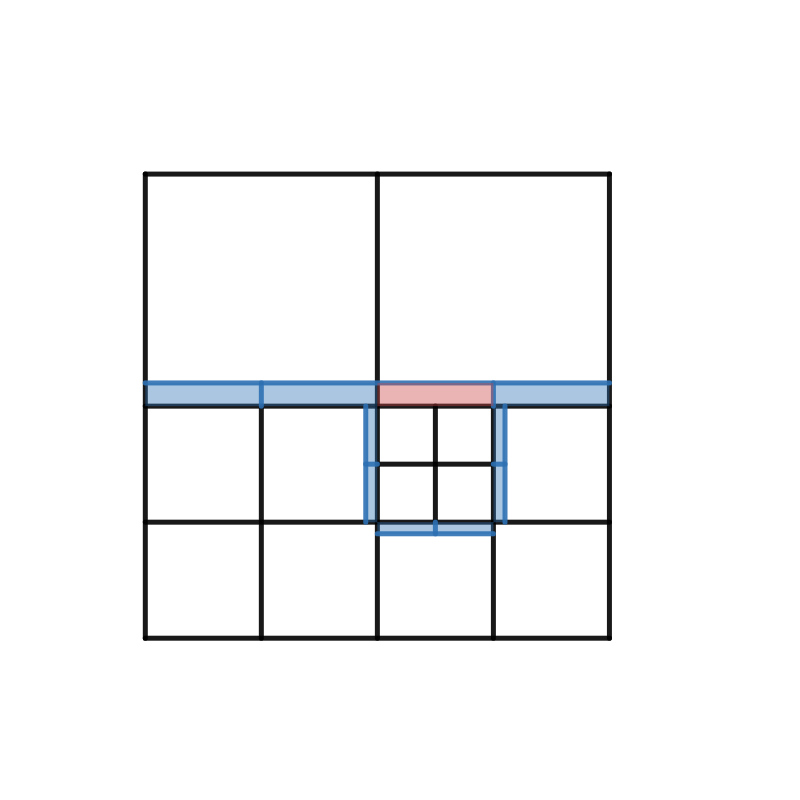
\includegraphics[width=0.5\textwidth]{octree_neighbor_error.png}
  \label{fig:octree_neighbor_error}
\end{SCfigure}
To rectify this issue, a refinement strategy is used to ensure that cases like this do not occur within the octree. When the octree needs to be modified, the following 4 steps are performed in order:
\begin{enumerate}
  \item Traverse the octree, visiting every node. If a non-leaf node satisfies \texttt{shouldChop}, then flag it, but do not delete its children yet. If a leaf node satisfies \texttt{shouldSplit}, then split it, creating 8 new leaf nodes. The newly created leaves will also be traversed in this step, allowing more than one layer of the octree to be generated at once.
  
  \begin{lstlisting}[language=C++,label={flagsplitphase},caption={The first stage in the octree refinement process.}]
bool Octree::flagSplitPhase(glm::vec3 inPos) {
  bool result = false;
  if (shouldChop(inPos)) {
    flagged = true;
    result = true;
  } 
  if (shouldSplit(inPos)) {
    split();
    result = true;
  }
  if (!isLeaf) {
    for (int i = 0; i <= 1; i++) {
      for (int j = 0; j <= 1; j++) {
        for (int k = 0; k <= 1; k++) {
          result |= myChildren[i][j][k]->flagSplitPhase(inPos);
        }
      }
    }
  }
  return result;
}
  \end{lstlisting}
  \item  If the first step changed the structure of the octree, or flagged any nodes, check whether any nodes have neighbors which are more than one level of detail higher, using the \texttt{getNeighbor} function described in listing \ref{octree_neighbor}. If this occurs on a leaf node, then split the node into its 8 children, otherwise unflag it, if it was flagged. This flagging prevents octree nodes and the corresponding geometry from being deleted in the first step, then immediately recreated in the subsequent steps. Performing this step may create inconsistencies elsewhere, so it is performed repeatedly, until no more changes are made.

  \begin{lstlisting}[language=C++,label={refinephase},caption={The second stage in the octree refinement process, \texttt{refine}. The array \texttt{edgeNeighbors} corresponds to the relative positions of the 6 neighboring nodes at the same level, and the variable \texttt{childPosition} gives the position of the child to check in each neighbor. The flow of this code is designed such that exactly the 4 children of the neighboring node that touch the chunk in this node are checked.}] 
//refine the octree - if a neighbor directly adjacent, smaller by more than one exists, split this
//return true if no refinements were made
bool Octree::refine() {
  bool result = true;
  glm::ivec3 edgeNeighbors[6] = {
    glm::ivec3(0,0,1),
    glm::ivec3(0,0,-1),
    glm::ivec3(0,1,0),
    glm::ivec3(0,-1,0),
    glm::ivec3(1,0,0),
    glm::ivec3(-1,0,0)
  };
  for (int n = 0; n < 6; n++) {
    Octree* neighbor = getNeighbor(edgeNeighbors[n]);
    if (neighbor && !neighbor->isLeaf) {
      for (int i = 0; i <= 1; i++) {
        for (int j = 0; j <= 1; j++) {
          for (int k = 0; k <= 1; k++) {
            glm::ivec3 childPosition = glm::ivec3(
              edgeNeighbors[n].x == 0 ? i : (1-edgeNeighbors[n].x)/2,
              edgeNeighbors[n].y == 0 ? j : (1-edgeNeighbors[n].y)/2,
              edgeNeighbors[n].z == 0 ? k : (1-edgeNeighbors[n].z)/2
            );
            Octree* child = neighbor->childFromVec3(childPosition);
            //if child exists, and is not a leaf, then this chunk is inconsistent
            //if it is a leaf, split it, otherwise just unflag it
            if (child && !child->isLeaf) {
              if (isLeaf && myDetailLevel < Config::get<int>("octree_max_depth")) {
                result = false;
                split();
              } else {
                flagged = false;
              }
              //once we know we are splitting, dont bother checking the other options
              //break 4 loops is easiest with a goto
              goto REFINE_CHILDREN;
            }
            if (edgeNeighbors[n].z != 0) break;
          }
          if (edgeNeighbors[n].y != 0) break;
        }
        if (edgeNeighbors[n].x != 0) break;
      }
    }
  }
  
  REFINE_CHILDREN:
  if (!isLeaf) {
    for (int i = 0; i <= 1; i++) {
      for (int j = 0; j <= 1; j++) {
        for (int k = 0; k <= 1; k++) {
          result &= myChildren[i][j][k]->refine();
        }
      }
    }
  }
  return result;
}
  \end{lstlisting}

  \item Once the previous step is complete, delete the children of any nodes which are still flagged. 
  
  \begin{lstlisting}[language=C++,label={deleteregenphase},caption={The third stage in the octree refinement process.}]
void Octree::deleteRegenPhase() {
  //chop chunks that shouldnt be there
  if (flagged) {
    chop();
    flagged = false;
  }
  if (!isLeaf) {
    for (int i = 0; i <= 1; i++) {
      for (int j = 0; j <= 1; j++) {
        for (int k = 0; k <= 1; k++) {
          myChildren[i][j][k]->deleteRegenPhase();
        }
      }
    }
  }  
}
  \end{lstlisting}
  \item Finally, generate geometry for all new leaves, and all leaves that needed regeneration, for example if the geometry inside them has changed. Also regenerate geometry for all leaves where \texttt{edgeIndex} has changed, so that cracks do not appear after changing the level of detail of a neighboring chunk.
  \begin{lstlisting}[language=C++,label={generateallchunks},caption={The fourth stage in the octree refinement process.}]
void Octree::generateAllChunks(bool force) {
  //needed so we have the shape of the octree before generating chunks that rely on it
  unsigned int E = getEdgeIndex();

  if (isLeaf) {
    if (!hasChunk || E != edgeIndex || force || needsRegen) {
      edgeIndex = E;
      generateMarchingChunk(edgeIndex);
    }
  } else {
    for(int i = 0; i <= 1; i++) {
      for(int j = 0; j <= 1; j++) {
        for(int k = 0; k <= 1; k++) {
          myChildren[i][j][k]->generateAllChunks();
        }
      }
    }
  }
}
  \end{lstlisting}
\end{enumerate}

\section{Terrain Modification}
\subsection{Method of Terrain Modification}
Since the parallel Transvoxel algorithm runs so efficiently, it is possible to regenerate significant portions of geometry in between frames, and so real-time terrain editing is achievable. 

We will proceed by dynamically adding primitive shapes to the SDF itself, using the set-theoretical operations discussed in section \ref{section:sdf}. This means that the shape represented by the SDF changes, so the generated geometry also changes, regardless of the level of detail it is generated at. It also means that we do not have to perform any subsequent transformations to the geometry, after the Transvoxel algorithm has generated it.

\subsection{Adding Primitives to the SDF}
\label{section:modification_implementation}

To implement terrain modification, the \texttt{Brush} interface is used. Each \texttt{Brush} object contains information about a shape that has been added to the world, and has 2 methods which are overridden for each type of shape. The first method is \texttt{getBoundingBox()}, which returns an axis-aligned bounding box such that the shape lies entirely within the box. The second is \texttt{getBrushParams()}, which returns a \texttt{BrushParams} object containing all of the parameters required to add this shape to the SDF. 

For example, it may contain the radius of a sphere, or the control points and thickness of a shape defined by a Bezier spline. It always contains the values \texttt{bottom} and \texttt{top}, which correspond to diagonally opposite corners of the bounding box, \texttt{type}, a constant denoting the type of shape, and \texttt{mode}, a constant describing whether the shape should be added or subtracted from the SDF.

A new \texttt{Brush} object is created each time a shape is added to the world. Each \texttt{Octree} node stores a list of pointers to the \texttt{Brush} objects that are inside the region the node represents. 

\begin{lstlisting}[language=C++,label={edit_add},caption={Code to add a new brush into the octree. The brush is added recursively to lists at all levels, so each leaf has a list of exactly the brushes that are partially inside it. The flag \texttt{needsRegen} indicates that the geometry within the chunk has changed.}]
void Octree::insertBrush(Brush* b) {
  myBrushes.push_back(b);
  if (isLeaf) {
    needsRegen = true;
    return;
  }
  for (int i = 0; i <= 1; i++) {
    for (int j = 0; j <= 1; j++) {
      for (int k = 0; k <= 1; k++) {
        Octree* thisChild = myChildren[i][j][k];
        if (b->getBoundingBox().intersects(thisChild->getBoundingBox())) {
          thisChild->insertBrush(b);
        }
      }
    }
  }
}
\end{lstlisting}

When the octree is modified, it is necessary to update the lists of the newly created nodes. To do this, the \texttt{split()} function is modified to update the brush lists of each child.

\begin{lstlisting}[language=C++,label={edit_split},caption={Snippet from \texttt{split}, showing how brushes are added to child nodes, when they are created.}]
for(int i = 0; i <= 1; i++) {
  for(int j = 0; j <= 1; j++) {
    for(int k = 0; k <= 1; k++) {
      Octree* thisChild = new Octree(0.5f * mySize,myPosition + mySize * 0.5f * glm::vec3(i,j,k), myDetailLevel + 1,myGenerator,this,glm::uvec3(i,j,k));
      auto it = myBrushes.begin();
      while (it != myBrushes.end()) {
        if ((*it)->getBoundingBox().intersects(thisChild->getBoundingBox())) {
          thisChild->insertBrush(*it);
        }
        it++;
      }
      myChildren[i][j][k] = thisChild;
    }
  }
}
\end{lstlisting}

Each brush type has an SDF and normal function implementation in GLSL. When geometry is generated for a chunk, the \texttt{BrushParams} objects corresponding to the brushes in the corresponding node are passed to the generation algorithm, and are used in the order they are passed, to modify the SDF via set union or subtraction. The normal function is computed by taking the shape which produces the smallest value of the SDF, and returning the normal function for that shape. Both the SDF and normal suffer from inaccuracies when a non-exact SDF is very far from the actual distance value, and in extreme cases, the resulting inaccurate interpolation can lead to cracks appearing in the geometry. Figure \ref{fig:inaccurate_sdf} shows an example of an SDF that exhibits this problem. However, with careful choices of SDF, in most cases it produces an acceptable result.

\begin{figure}[H]
  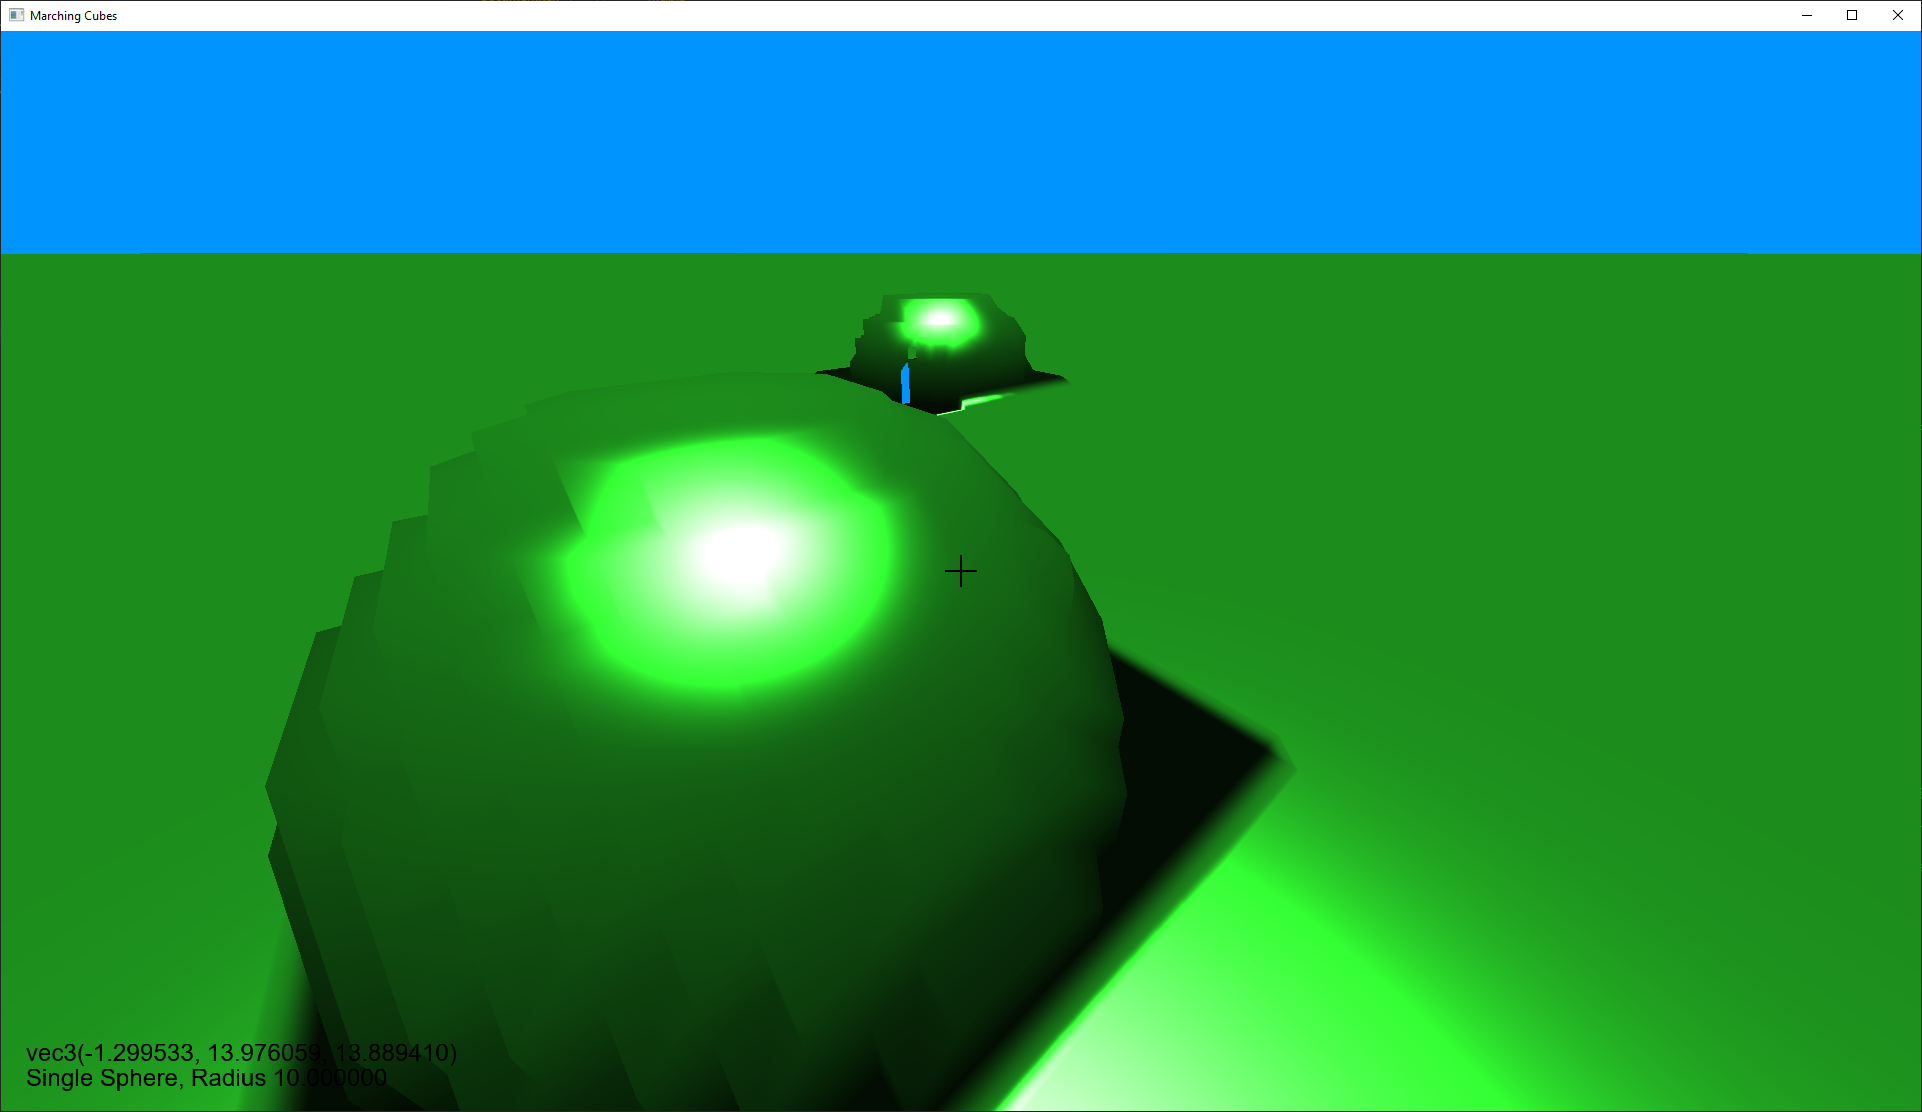
\includegraphics[width=\textwidth]{inaccurate_sdf.png}
  \caption{An example of an inaccurate sphere SDF on an accurate plane SDF. Here the value of the SDF has been scaled to be much smaller than it should be. The incorrect SDF has been chosen for interpolation, resulting in the blocky appearance of the sphere, and cracks on the further away sphere, where the level of detail changes. This also results in the incorrect normal being used, as shown by the dark patches underneath the spheres.}
  \label{fig:inaccurate_sdf}
\end{figure}

For efficiency reasons, an SDF is only considered when the grid cell being worked on lies within its bounding box,
preventing unneccesary evaluation of SDFs that will not affect the geometry within the cell. This introduces discontinuities in the overall SDF being computed, and for this reason, it is necessary to enforce that the bounding box always contains the grid cells containing geometry generated for the brush.

\subsection{Interactive Terrain Modification}
User interaction with the terrain modification system uses a set of pre-defined actions, defined through classes derived from a base \texttt{Action} class, shown in listing \ref{action_methods}.

\begin{lstlisting}[language=C++,label={action_methods},caption={Methods of the \texttt{Action} class responsible for handling user interaction.}]
virtual void onMouseDown(glm::vec3 pos) {};
virtual void onMouseUp(glm::vec3 pos) {};
virtual void onMouseHold(glm::vec3 pos) {};
virtual void onCancel() {};
virtual void increaseSize() {};
virtual void decreaseSize() {};

virtual void handleInput(glm::vec3 placePos);
\end{lstlisting}
These functions are designed to be overridden, to implement the corresponding functionality. The argument to the first 3 is the in-world position at which the mouse is pointing. The method \texttt{onCancel} is called when the action has been cancelled, to clean up any state that has been created, for example in a more complex action that may store intermediate control points. The methods \texttt{increaseSize} and \texttt{decreaseSize} provide a standard way of increasing and decreasing the size of a shape, for example changing the radius of a sphere, or thickness of a spline curve. The final method, \texttt{handleInput}, allows more general input for an action, which is useful for actions that require more input than the options given in the other functions. It has a default implementation, which calls the other functions, that can be overridden.
\begin{lstlisting}[language=C++,label={action_handleinput},caption={Default implementation of \texttt{handleInput}.}]
void Action::handleInput(glm::vec3 placePos) {
  //default input handling for an action
  if (Controller::getKeyState(Window::window,GLFW_KEY_LEFT_BRACKET)) {
    decreaseSize();
  }
  if (Controller::getKeyState(Window::window,GLFW_KEY_RIGHT_BRACKET)) {
    increaseSize();
  }
  if (Controller::mousePressed(Window::window,GLFW_MOUSE_BUTTON_LEFT)) {
    onMouseDown(placePos);
  } else if (Controller::getMouseState(Window::window,GLFW_MOUSE_BUTTON_LEFT)) {
    onMouseHold(placePos);
  } else if (Controller::mouseReleased(Window::window,GLFW_MOUSE_BUTTON_LEFT)) {
    onMouseUp(placePos);
  }
}
\end{lstlisting}

The generic \texttt{Brush} and \texttt{Action} interfaces makes it quick to implement new shapes, since the interfaces just need to be filled out with the required brush parameters and controller code, respectively. The only complex addition is the definition of the SDF and normal function, which is different for every shape.

\subsubsection{Raycasting}
\label{section:raycasting}
To determine where a brush should be placed, we perform a raycast from the camera in the look direction. We take advantage of the structure of the octree to do this efficiently, considering only leaf nodes where the ray passes through their bounding box. For each of these nodes, we perform ray-triangle intersection tests to determine the closest point of intersection to the camera, using a library function. Since the geometry data is generated on the GPU, it first needs to be copied to the CPU.

\begin{lstlisting}[language=C++,label={mapgeometry},caption={Snippet from the procedure \texttt{mapGeometry} to copy geometry data for a chunk from the GPU to the array \texttt{mappedTriangles}. \texttt{isMapped} is an atomic boolean storing whether \texttt{mapGeometry} has already been called for this chunk.}]
if (!isMapped.load()) {
  glBindBuffer(GL_SHADER_STORAGE_BUFFER, vertexBuffer);
  mappedTriangles.resize(myGeometrySize);
  glGetBufferSubData(GL_SHADER_STORAGE_BUFFER,0,myGeometrySize * sizeof(glm::vec4),mappedTriangles.data());
  isMapped.store(true);
}
\end{lstlisting}

It would be possible to perform ray-triangle intersection tests within an OpenGL compute shader, removing the need for the geometry data to be copied to the CPU. However, this copying will need to be done for physics simulation anyway, and is only done once per chunk of geometry, this method will be sufficient.

\subsubsection{Example Brush Implementations}
\label{example_brushes}
Any shape for which an SDF and normal function can be derived may be implemented as a brush, using the method described in section \ref{section:modification_implementation}. A good resource for SDF implementations is the article by Inigo Quilez referenced in section \ref{section:sdf}~\cite{quilez:sdf}. It is also necessary to provide a normal function for each SDF. In some cases, the partial derivatives can be computed exactly, particularly when the SDF has a simple form. For example, the SDF of a sphere with radius 1, centered at the origin, is $f\left(x,y,z\right) = \sqrt{x^2+y^2+z^2}-1$. The gradient vector at point $\left(x,y,z\right)$ is $\nabla f = \left(\frac{x}{\sqrt{x^2+y^2+z^2}},\frac{y}{\sqrt{x^2+y^2+z^2}},\frac{z}{\sqrt{x^2+y^2+z^2}}\right)$. In this case, the gradient happens to already have length 1, but if it is not, it should be normalised with the GLSL \texttt{normalize} function. It is always possible to approximate the normal of an SDF numerically, however this can be computationally expensive, because it requires multiple evaluations of the SDF.

\begin{lstlisting}[language=C++,label={numerical_gradient},caption={Approximation of the normal of an SDF, using the method of finite differences.}]
vec3 normal(vec3 inPos) {
  //numerical normal of more complex distance function
  float eps = 0.001;
  vec3 dx = inPos + vec3(eps,0,0);
  vec3 dy = inPos + vec3(0,eps,0);
  vec3 dz = inPos + vec3(0,0,eps);

  float f  = distance(inPos);
  float fx = distance(dx);
  float fy = distance(dy);
  float fz = distance(dz);
  return normalize(vec3((fx-f)/eps, (fy-f)/eps, (fz-f)/eps));
}
\end{lstlisting}

\paragraph{Example Shape: Ellipsoid}
Another article by Inigo Quilez~\cite{quilez:ellipsoid} lists various approximate SDFs for ellipsoids. Listing \ref{ellipsoid_sdf} shows my transformation of the first SDF listed in this article into an SDF representing an ellipsoid at any given point in space, as well as a normal function, which has been derived by computing the gradient of this SDF.

\begin{lstlisting}[language=C++,label={ellipsoid_sdf},caption={Approximate SDF and normal function for an ellipsoid.}]
float ellipsoid_distance(vec3 inPos, vec4 location, vec4 radius) {
  float k1 = length((inPos-location.xyz)/radius.xyz);
  return (k1-1.0) * min(min(radius.x,radius.y),radius.z);
}

vec3 ellipsoid_normal(vec3 inPos, vec4 location, vec4 radius) {
  float k1 = length((inPos-location.xyz)/radius.xyz);
  return normalize(1.0/k1 * (inPos.xyz - location.xyz) / (radius.xyz * radius.xyz));
}
\end{lstlisting}
Figure \ref{fig:editing_ellipsoids} shows a number of ellipsoids of various sizes being placed.
\begin{figure}[H]
  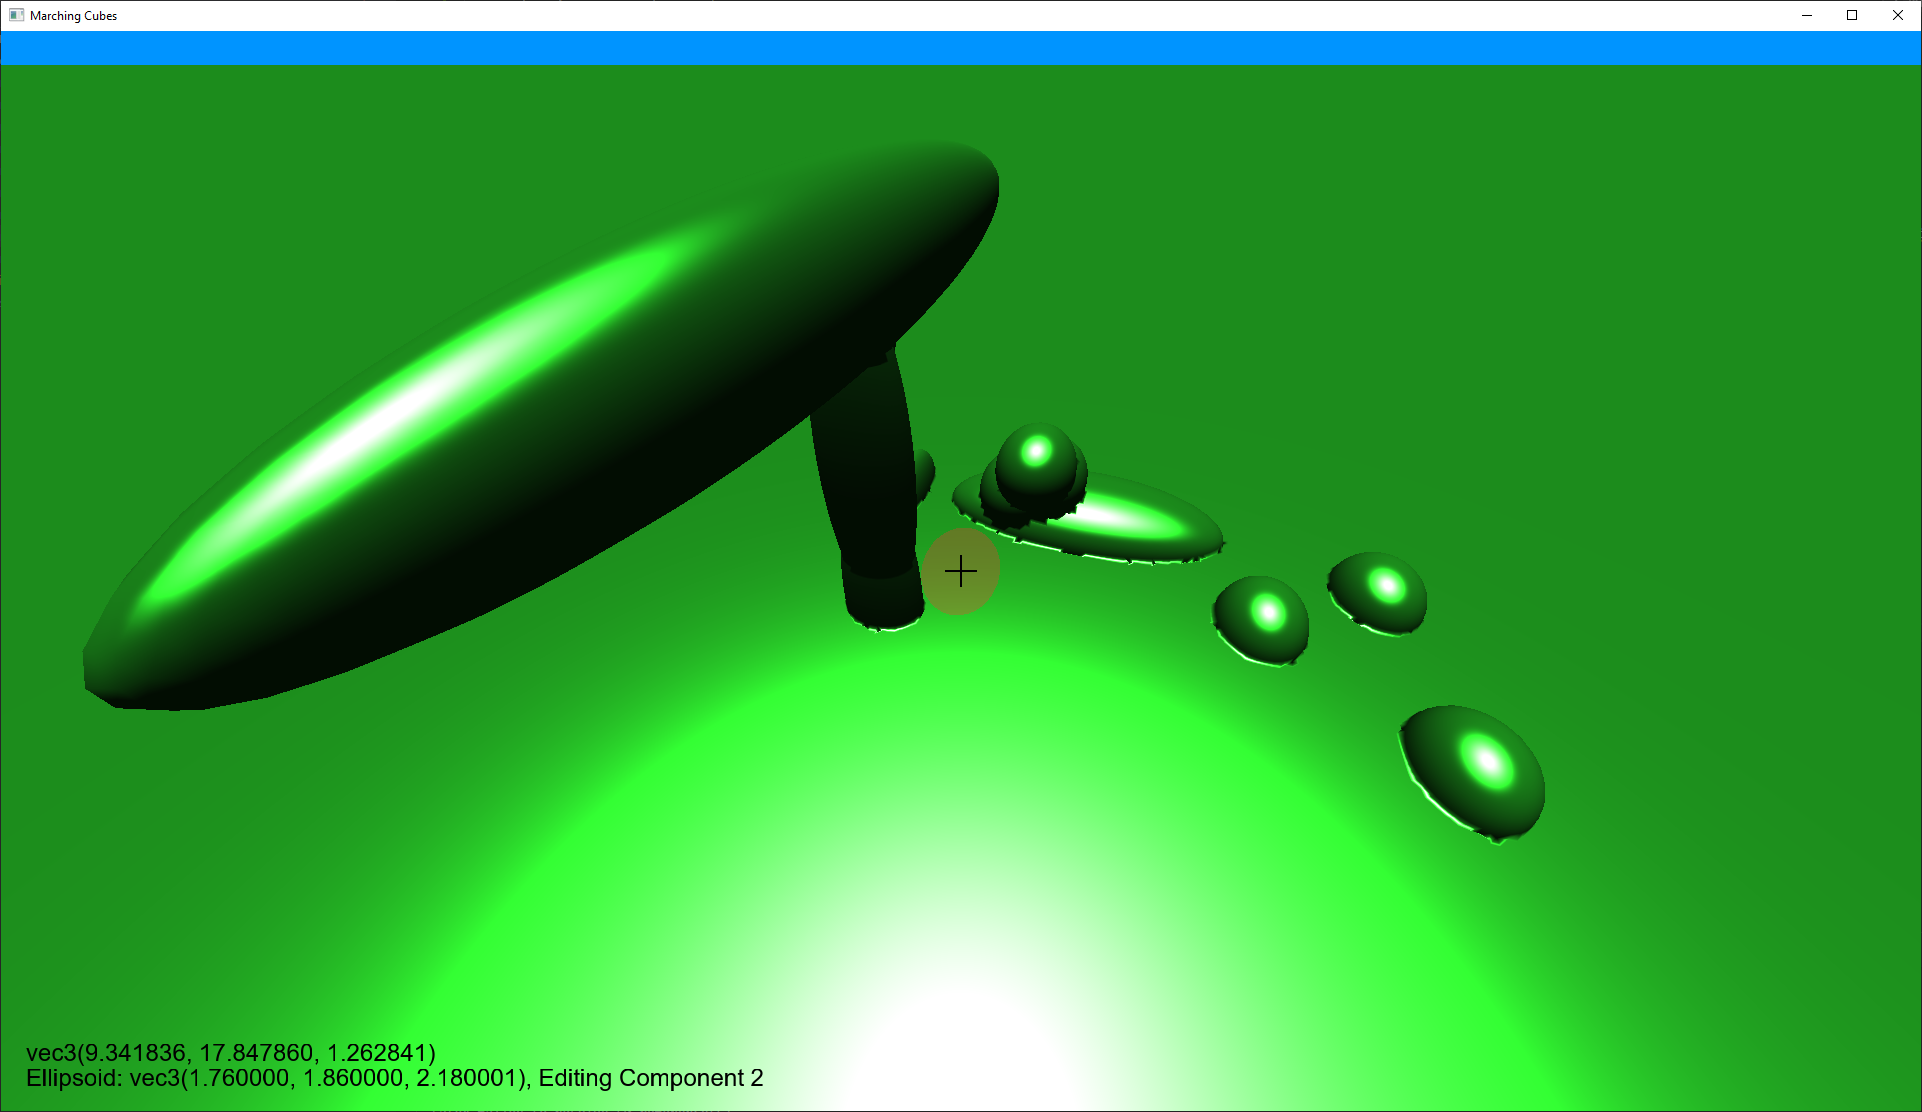
\includegraphics[width=\textwidth]{editing_ellipsoids}
  \caption{Multiple ellipsoid brushes of different sizes. Due to the sharp edges between an ellipsoid and a plane, small shading artifacts are visible.}
  \label{fig:editing_ellipsoids}
\end{figure}

\paragraph{Shapes Using Bezier Curves}
\subparagraph{Exact Method} %TODO - reference on bezier interpolation
To define a smooth curve between interpolation points, we will use Bezier interpolation. Intermediate control points are calculated between each consecutive pair of interpolation points, such that the section of curve between them is a cubic Bezier spline. Calculating the minimum distance to a Bezier curve is best done by minimising the value of a degree 6 polynomial. A general cubic Bezier is a cubic $c\left(t\right), t \in \left[0,1\right]$, and the value of the SDF at point $p$ is the minimum of $\| c\left(t\right) -p\|$. This minimum is found by differentiating $\| c\left(t\right) -p\|^2$, a degree 6 polynomial, to give a polynomial of degree 5.

Since it is impossible to solve a general degree 5 polynomial analytically, we instead use a numerical approach. We will use an existing implementation~\cite{kraus_2021} that uses interval approximation to find the first root, followed by polynomial long division to obtain the coefficients of a degree 4 polynomial, and finally computes the 4 remaining roots exactly. Once the minimum distance to the curve has been computed, It is simple to define a shape with a circular cross-section by defining a radius, such that points closer than that radius are considered inside, and points further away are considered outside. Figure \ref{fig:exact_bezier} shows an example of such a shape.
\begin{figure}[H]
  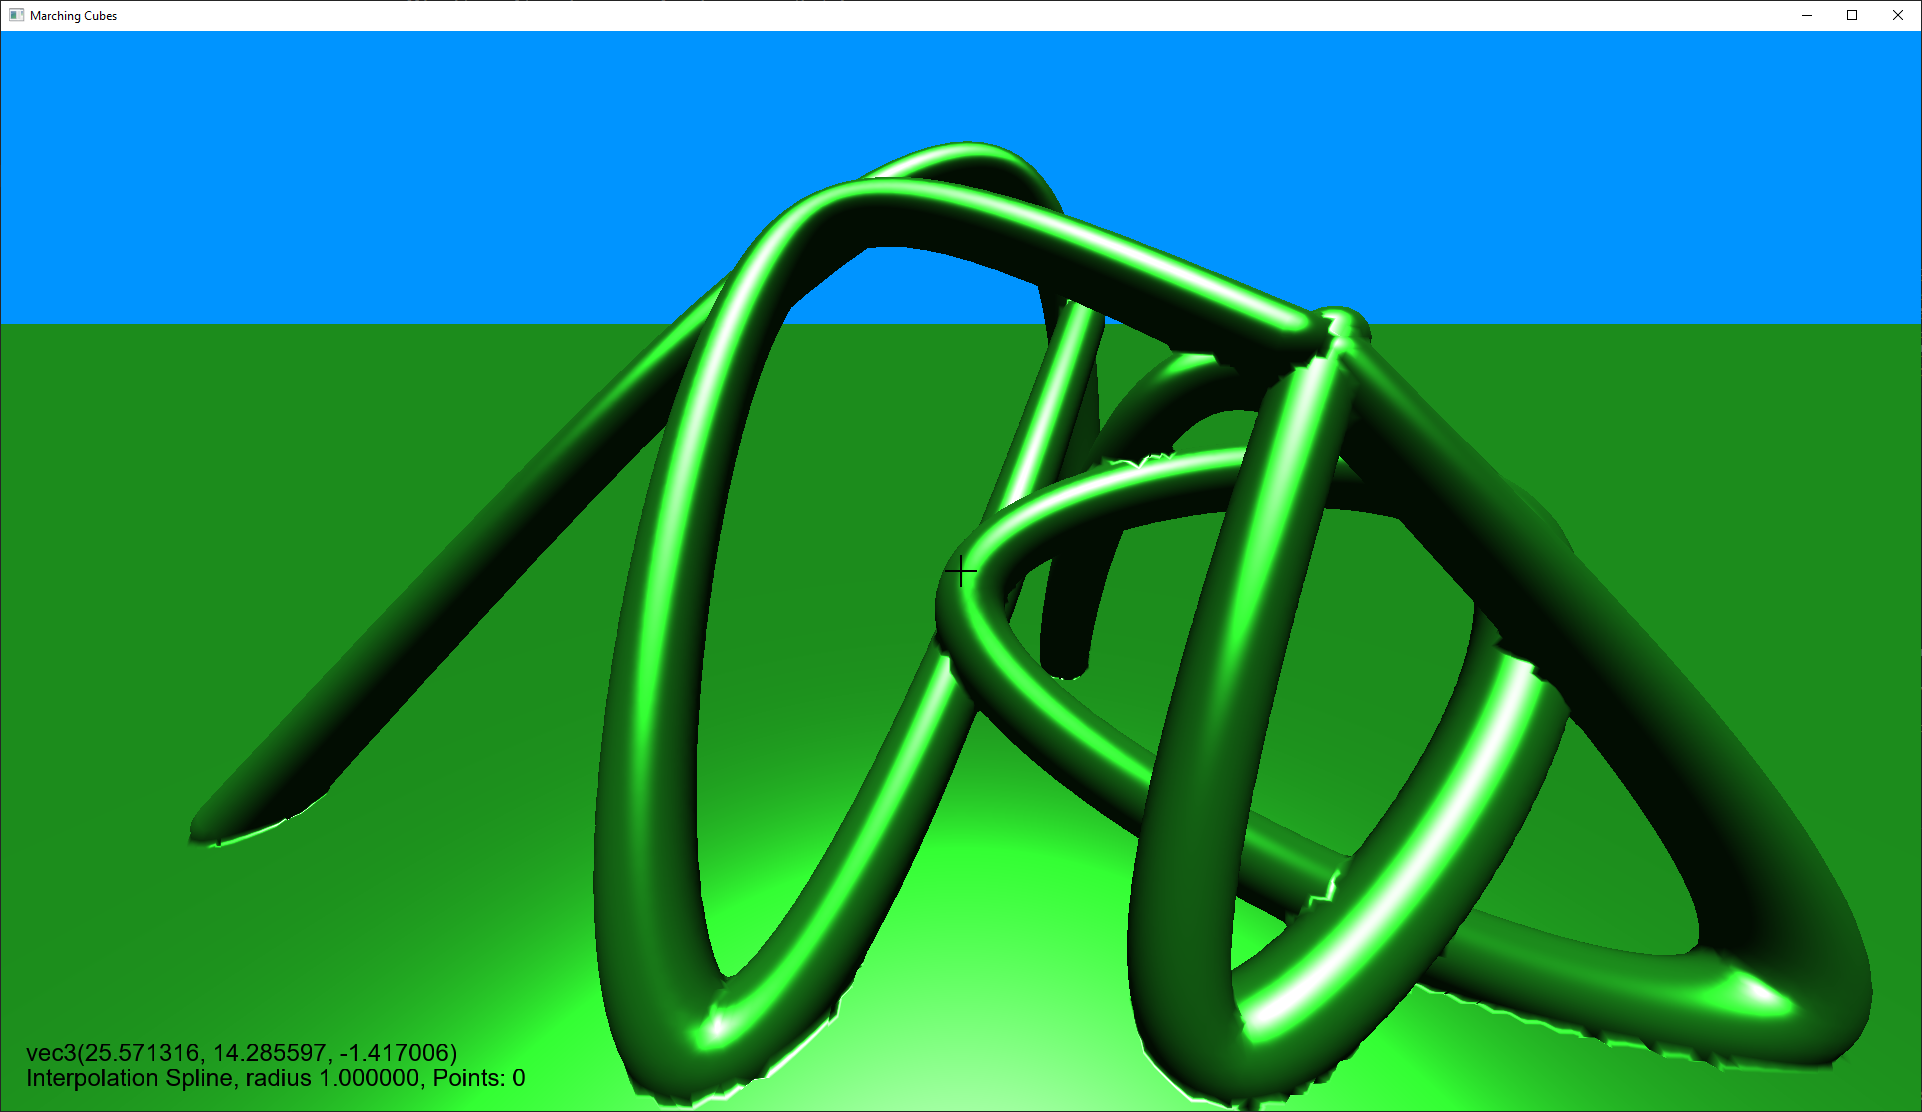
\includegraphics[width=\textwidth]{exact_bezier}
  \caption{A number of Bezier interpolation splines, using the exact SDF.}
  \label{fig:exact_bezier}
\end{figure}

There is no simple form for the gradient of this SDF, and so we use the numerical derivative as implemented in listing \ref{numerical_gradient}. Note however that this now requires solving 5 cubics for every SDF sample point.

\subparagraph{Approximate Method}
To avoid the complex computation that comes with finding the roots of a quintic, a Bezier spline can be approximated by a number of line segments. Each line segment can then be associated with an SDF that is simple to evaluate. For example, figure \ref{fig:spline_approximation} shows a comparison between an approximated spline, and a spline using the exact SDF.
\begin{figure}[H]
  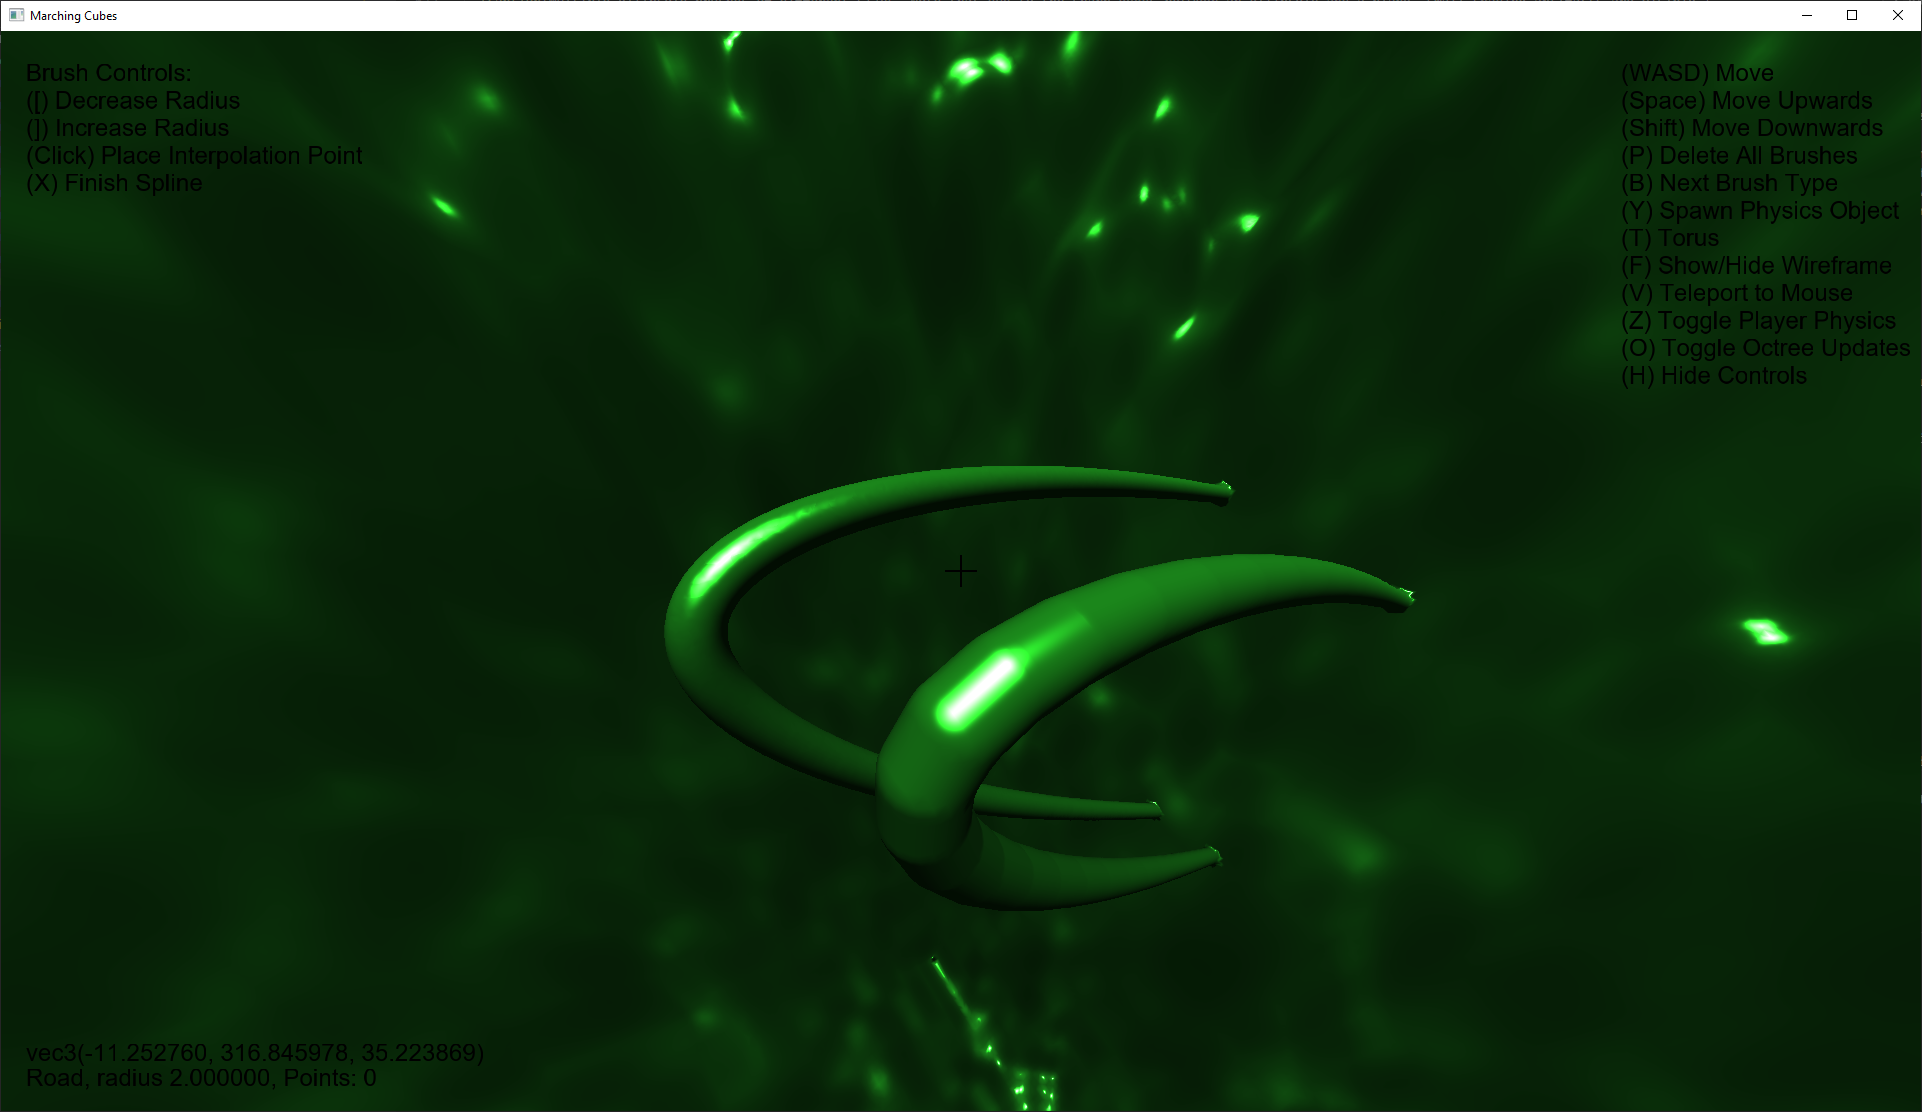
\includegraphics[width=\textwidth]{spline_approximation_2.png}
  \caption{Two similar interpolation splines. The nearest spline uses the approximation, whereas the farthest away spline uses the exact SDF. The linear segments of the approximation are more visible where the spline is most curved.}
  \label{fig:spline_approximation}
\end{figure}

Using approximation also allows for splines to be used to define more complex shapes, where calculating an exact SDF may be infeasible. Often the shape used for the line segment will result in jagged areas between line segments, when the shape is very curved. To solve this issue, at the ends of the shapes, we only consider the intersection, as demonstrated in figure \ref{fig:road_double}. 

Figure \ref{fig:bezier_roads} shows a shape generated with this method, using an SDF where each line segment along the spline is represented by a capsule intersected with a half-plane, to form a shape that is flat on top.

\begin{figure}[H]
  \caption{Left: Illustration of the union of 2 shapes at an angle, so there is a jagged overlap between them. Right: The same 2 shapes, considering only the intersection between the shapes at the end, giving a smoother appearance.}
  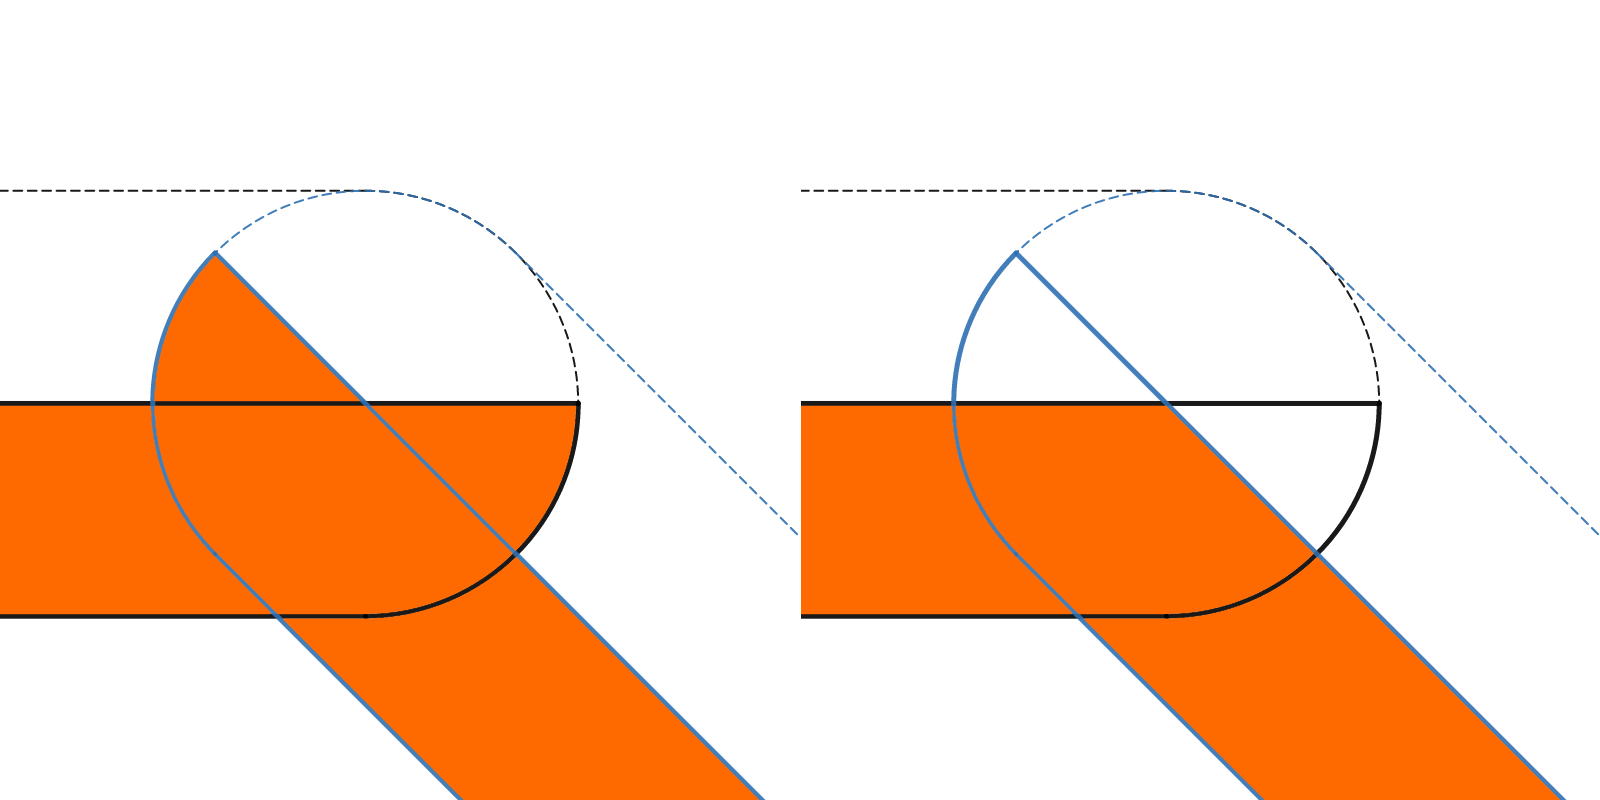
\includegraphics[width=\textwidth]{road_double.png}
  \label{fig:road_double}
\end{figure}

\begin{figure}[H]
  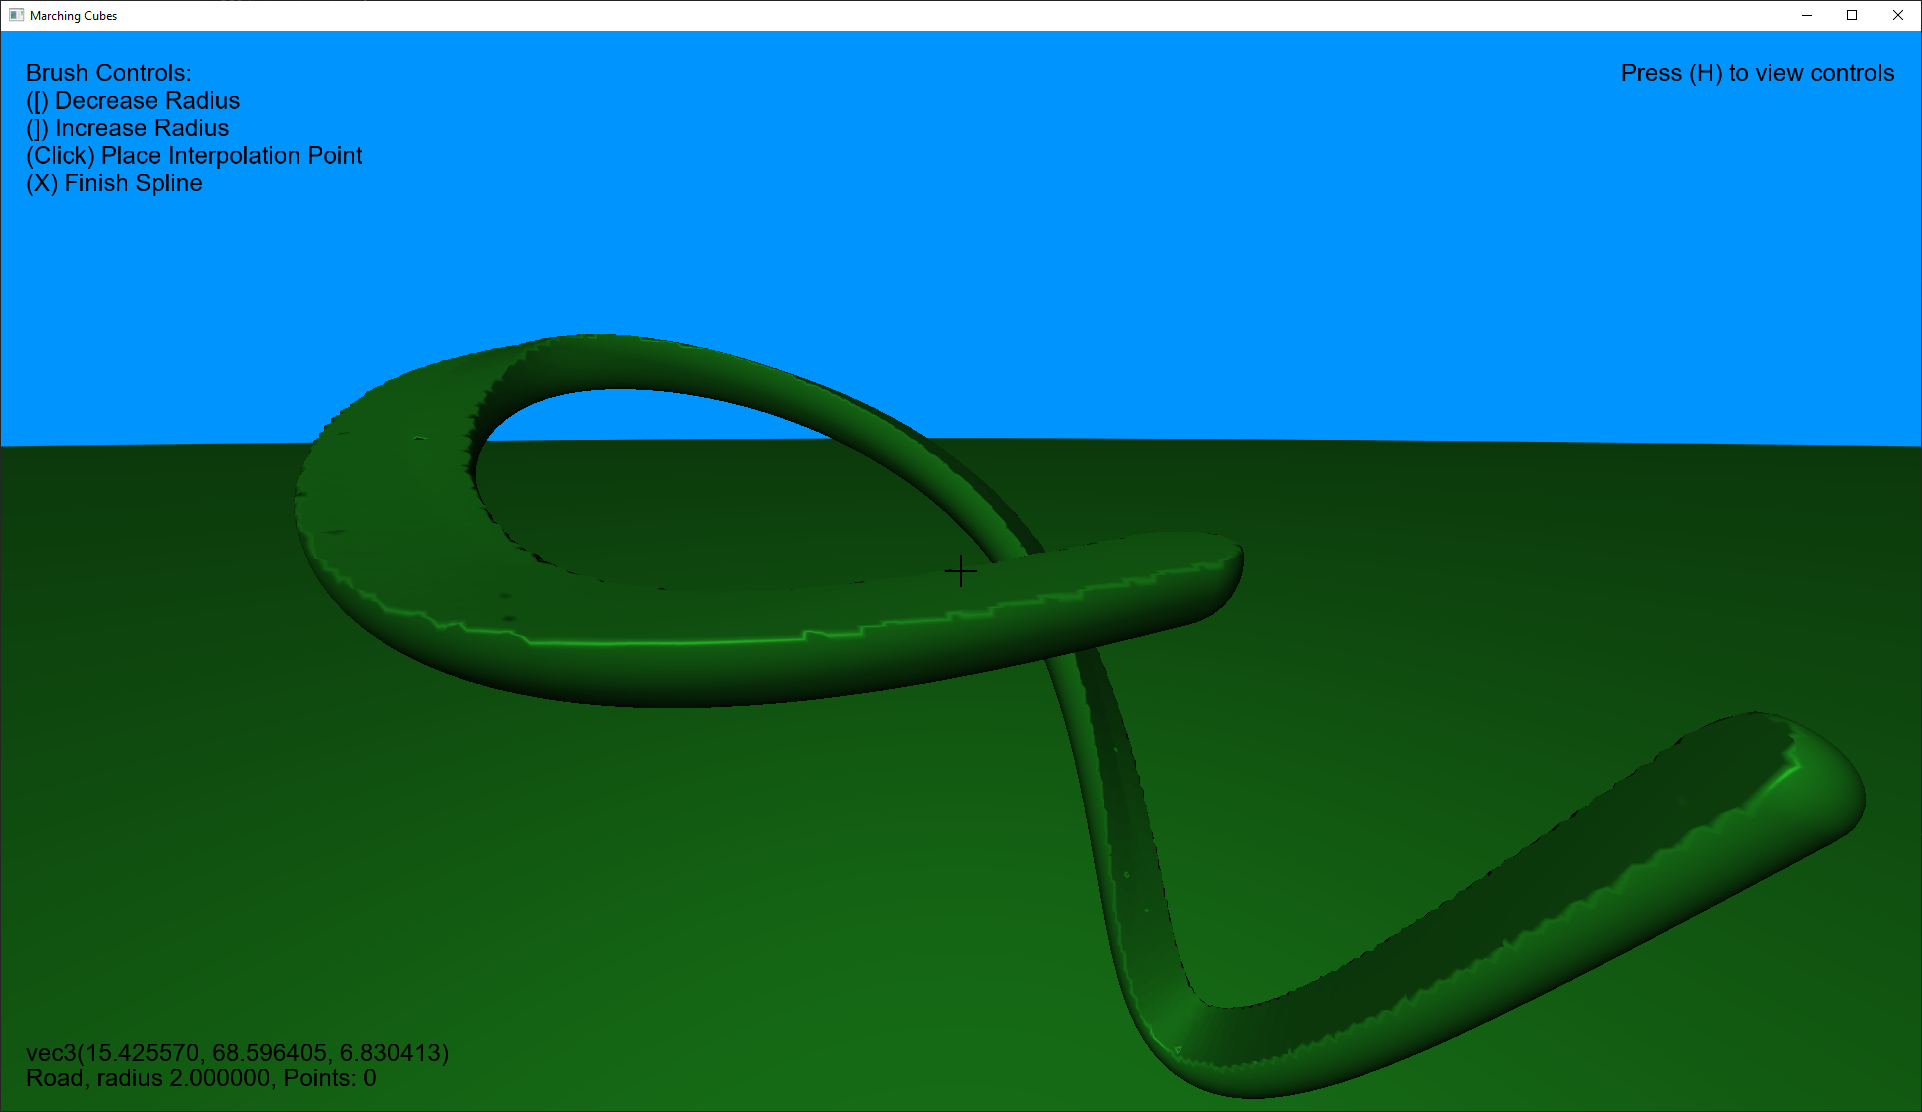
\includegraphics[width=\textwidth]{bezier_roads.png}
  \caption{Shape generated using splines having a more complex cross-section. Since each cubic curve in the interpolation spline is passed to the shader separately, the smoothing method was not used on the boundary between the curve segments, so some intersections between the shapes are still visible. Implementing this would require significant changes to the editing code, but would result in a smoother shape.}
  \label{fig:bezier_roads}
\end{figure}

Listing \ref{road_code} shows the GLSL code defining this SDF.

\begin{lstlisting}[language=C++,label={road_code},caption={\texttt{road\_distance} is the SDF for part of the shape defined by a single cubic Bezier curve. When an interpolation spline consisting of multiple curves is required, a \texttt{Brush} object is created for each.}]
//SDF of capsule between a and b, with radius r
float sdCapsule( vec3 p, vec3 a, vec3 b, float r ) {
  vec3 pa = p - a, ba = b - a;
  float h = clamp( dot(pa,ba)/dot(ba,ba), 0.0, 1.0 );
  return length( pa - ba*h ) - r;
}

//sdf of plane with normal n, passing through p0, offset in normal direction by h
float sdPlane(vec3 inPos, vec3 n, vec3 p0,float h) {
  return dot(n,inPos-p0)/length(n) - h;
}

//returns (distance, t value) for one line segment on the curve
vec2 road_segment(vec3 inPos, vec3 a, vec3 b, float r) {
  //normal in the plane containing line direction and up vector, perpendicular to direction
  vec3 planeDirection = b-a;
  vec3 planeNormal = vec3(
    -planeDirection.x*planeDirection.y,
    planeDirection.x * planeDirection.x + planeDirection.z * planeDirection.z, 
    -planeDirection.z*planeDirection.y
  );

  //proportion of radius the plane will be above the center - 0 for half-circle cross-section, 1 for circle cross-section
  float hProp = 0.2;

  //SDF value - intersect a capsule with a plane
  float capsuleDistance = sdCapsule(inPos,a,b,r);
  float planeDistance = sdPlane(inPos,planeNormal,a,hProp*r);
  float resDistance = max(capsuleDistance,planeDistance);

  //t value along the line a+t(b-a) such that p is closest
  float t = dot(inPos-a,b-a)/dot(b-a,b-a);
  return vec2(resDistance,t);
}

int roadResolution = 32;
float road_distance(vec3 inPos, vec4 A, vec4 B, vec4 C, vec4 D, float r) {
  //Approximation method
  vec2 dMin = vec2(1e4,0);
  int bestI = 0;
  for (int i = 0; i < roadResolution; i++) {

    float nt = i/float(roadResolution);
    float nt1 = (i+1.)/float(roadResolution);

    vec3 a = B3(nt ,A.xyz,B.xyz,C.xyz,D.xyz);
    vec3 b = B3(nt1,A.xyz,B.xyz,C.xyz,D.xyz);

    //bounding box with a little bit of wiggle room, so the very ends of the line are always generated properly
    vec4 bottom = min(a,b).xyzz - vec4(r * 1.1);
    vec4 top = max(a,b).xyzz + vec4(r * 1.1);

    if (inBox(bottom,top,inPos)) {
      vec2 segmentResult = road_segment(inPos,a,b,r);
      //store the closest distance and t value
      if (segmentResult.x < dMin.x) {
        dMin = segmentResult;
        bestI = i;
      }

    }
  }
    
  //not on one of the end caps - just return SDF
  if (dMin.y <=1. && dMin.y >= 0.) {
    return dMin.x;
  }
  //on an endcap, only return the part of the endcap that intersects with the next segment
  float nt, nt1;
  if (dMin.y > 1.) {
    //return intersection of endcap with next segment
    nt = (bestI+1.)/float(roadResolution);
    nt1 = (bestI+2.)/float(roadResolution);
  } else { //dMin.y < 0.
    // return intersection of endcap with previous segment
    nt = (bestI-1.)/float(roadResolution);
    nt1 = bestI/float(roadResolution);
  }
  //compute SDF of adjacent segment
  vec3 a = B3(nt ,A.xyz,B.xyz,C.xyz,D.xyz);
  vec3 b = B3(nt1,A.xyz,B.xyz,C.xyz,D.xyz);
  vec2 nextResult = road_segment(inPos,a,b,r);
  return max(nextResult.x,dMin.x);
}
\end{lstlisting}


\subsubsection{Limits of Terrain Modification}
\label{edit_limits}
This terrain modification system allows for a wide variety of shapes to be implemented. The efficiency improvements resulting from the use of the octree to prevent iteration over large lists of brushes, and the use of bounding boxes inside the GLSL shader means that a large number of brushes can exist at once, provided they are spread out. However, the number of brushes in the world grows without bound as editing occurs, meaning that slowdown is inevitable, particularly when the number of brushes in a single node becomes high, since this requires more work in the generation shader. This causes a stutter in between frames, when a large amount of geometry need to be regenerated. This can be reduced by limiting the speed of the user so that a large movement in between frames does not happen. There are other ways to address this, which we will discuss in section \ref{section:future_work}. Nevertheless, it is possible to modify the world with many thousands of brushes before significant slowdown occurs.

\section{Graphical User Interface}

To make editing more intuitive, a basic graphical user interface has been implemented. Text showing the camera position and currently enabled brush is displayed in the bottom left. A list of controls is displayed on the right, and can be hidden if necessary. Controls for the selected brush are shown on the top left. A crosshair is shown in the middle of the screen, to show the user what they are currently pointing at. When a brush is being placed, a preview is shown to the user, to help them understand what modification will be performed. To implement this, the methods \texttt{drawPreview}, \texttt{getDescription}, and \texttt{getDetails} have been added to the \texttt{Action} interface. Listing \ref{action_ui_methods} shows the implementation of these methods for drawing a sphere.

\begin{lstlisting}[language=C++,label={action_ui_methods},caption={The UI methods for the \texttt{SphereAction} class.}]
void SphereAction::drawPreview() {
  Preview::drawPreviewSphere(glm::vec3(radius),Window::placePos);
}

std::string SphereAction::getDescription() {
  return "Sphere, Radius " + std::to_string(radius);
}

std::string SphereAction::getDetails() {
  return "Brush Controls:\n"
         "([) Decrease Size\n"
         "(]) Increase Size\n"
         "(Click) Place Spheres";
}
\end{lstlisting}

Previews for shapes defined using Bezier splines are shown by approximating the curve with a series of cylinders. Some examples of the user interface are shown in figures \ref{fig:sphere_preview}, \ref{fig:cylinder_preview} and \ref{fig:spline_preview}.

\begin{figure}[H]
  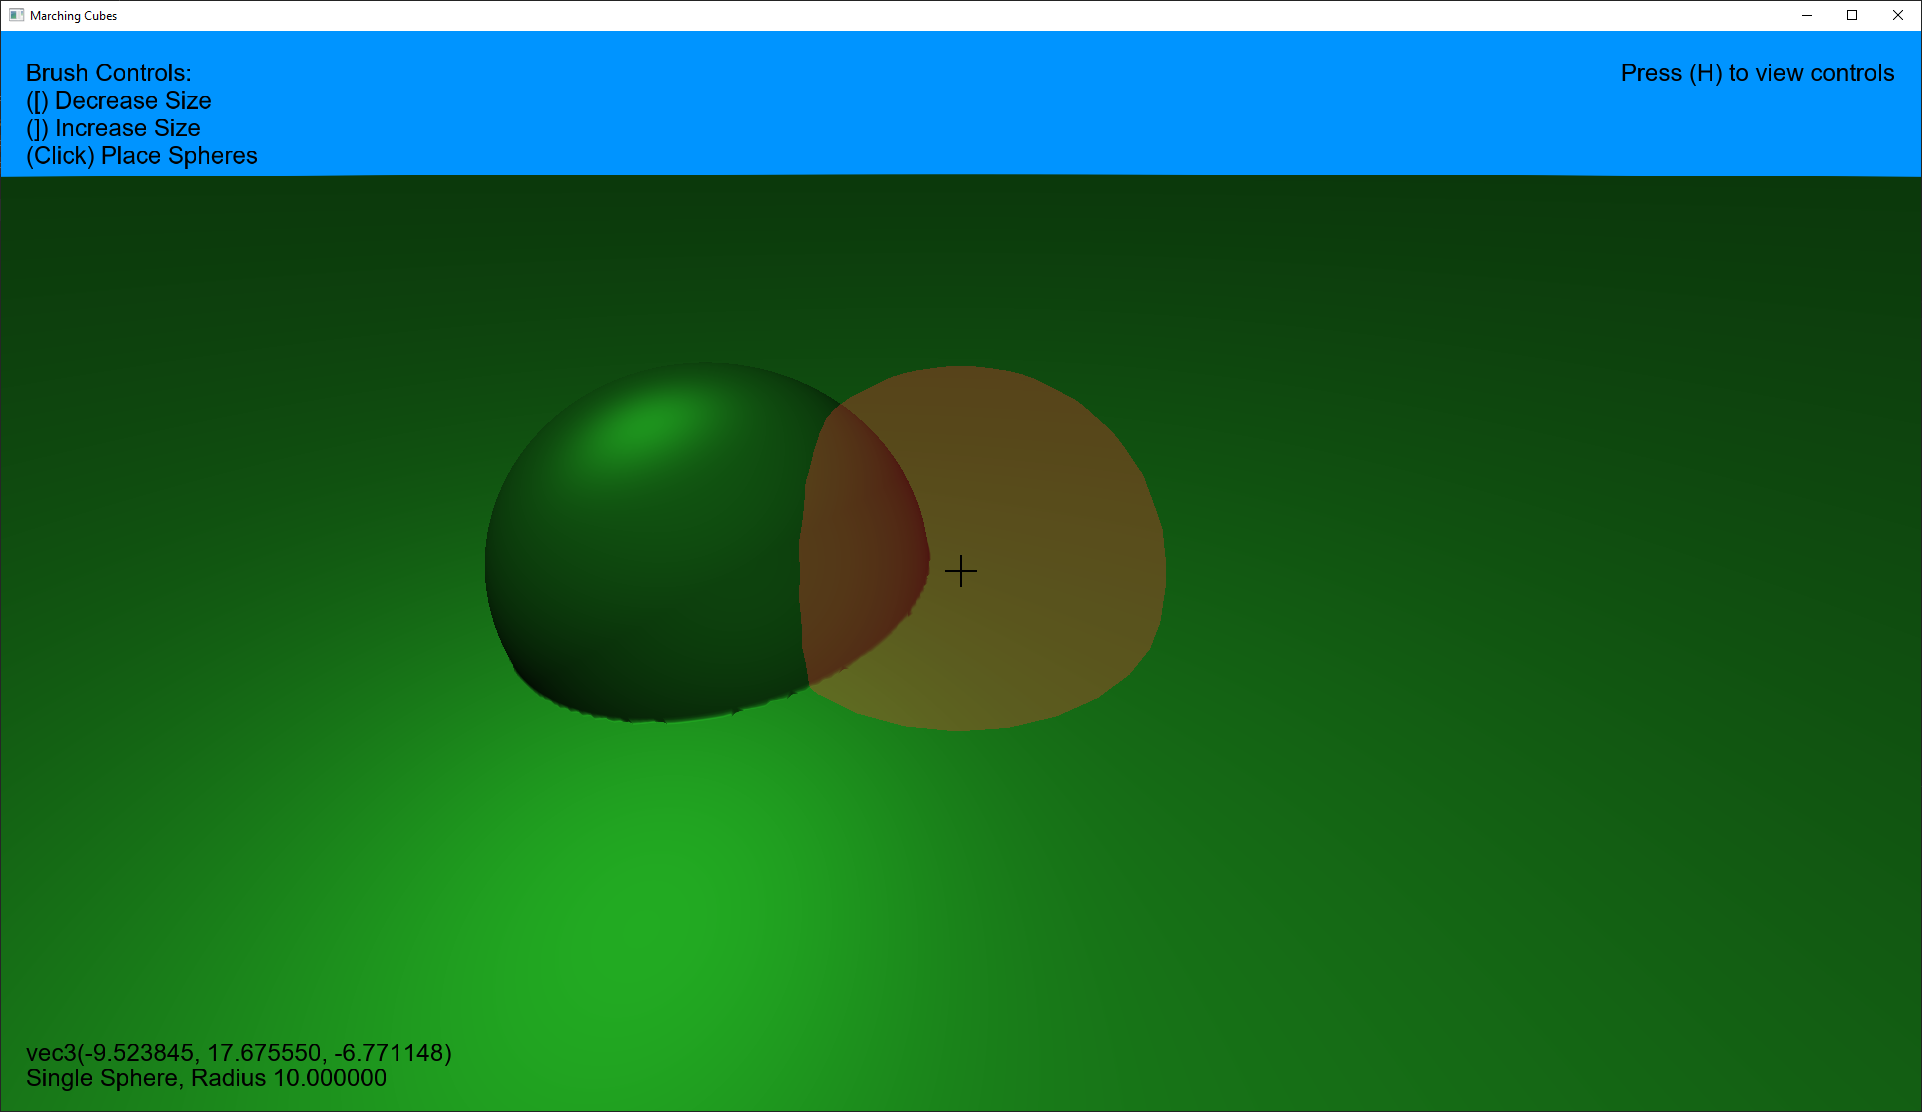
\includegraphics[width=\textwidth]{sphere_preview.png}
  \caption{Preview of a sphere about to be placed, next to a sphere that has already been placed.}
  \label{fig:sphere_preview}
\end{figure}
\begin{figure}[H]
  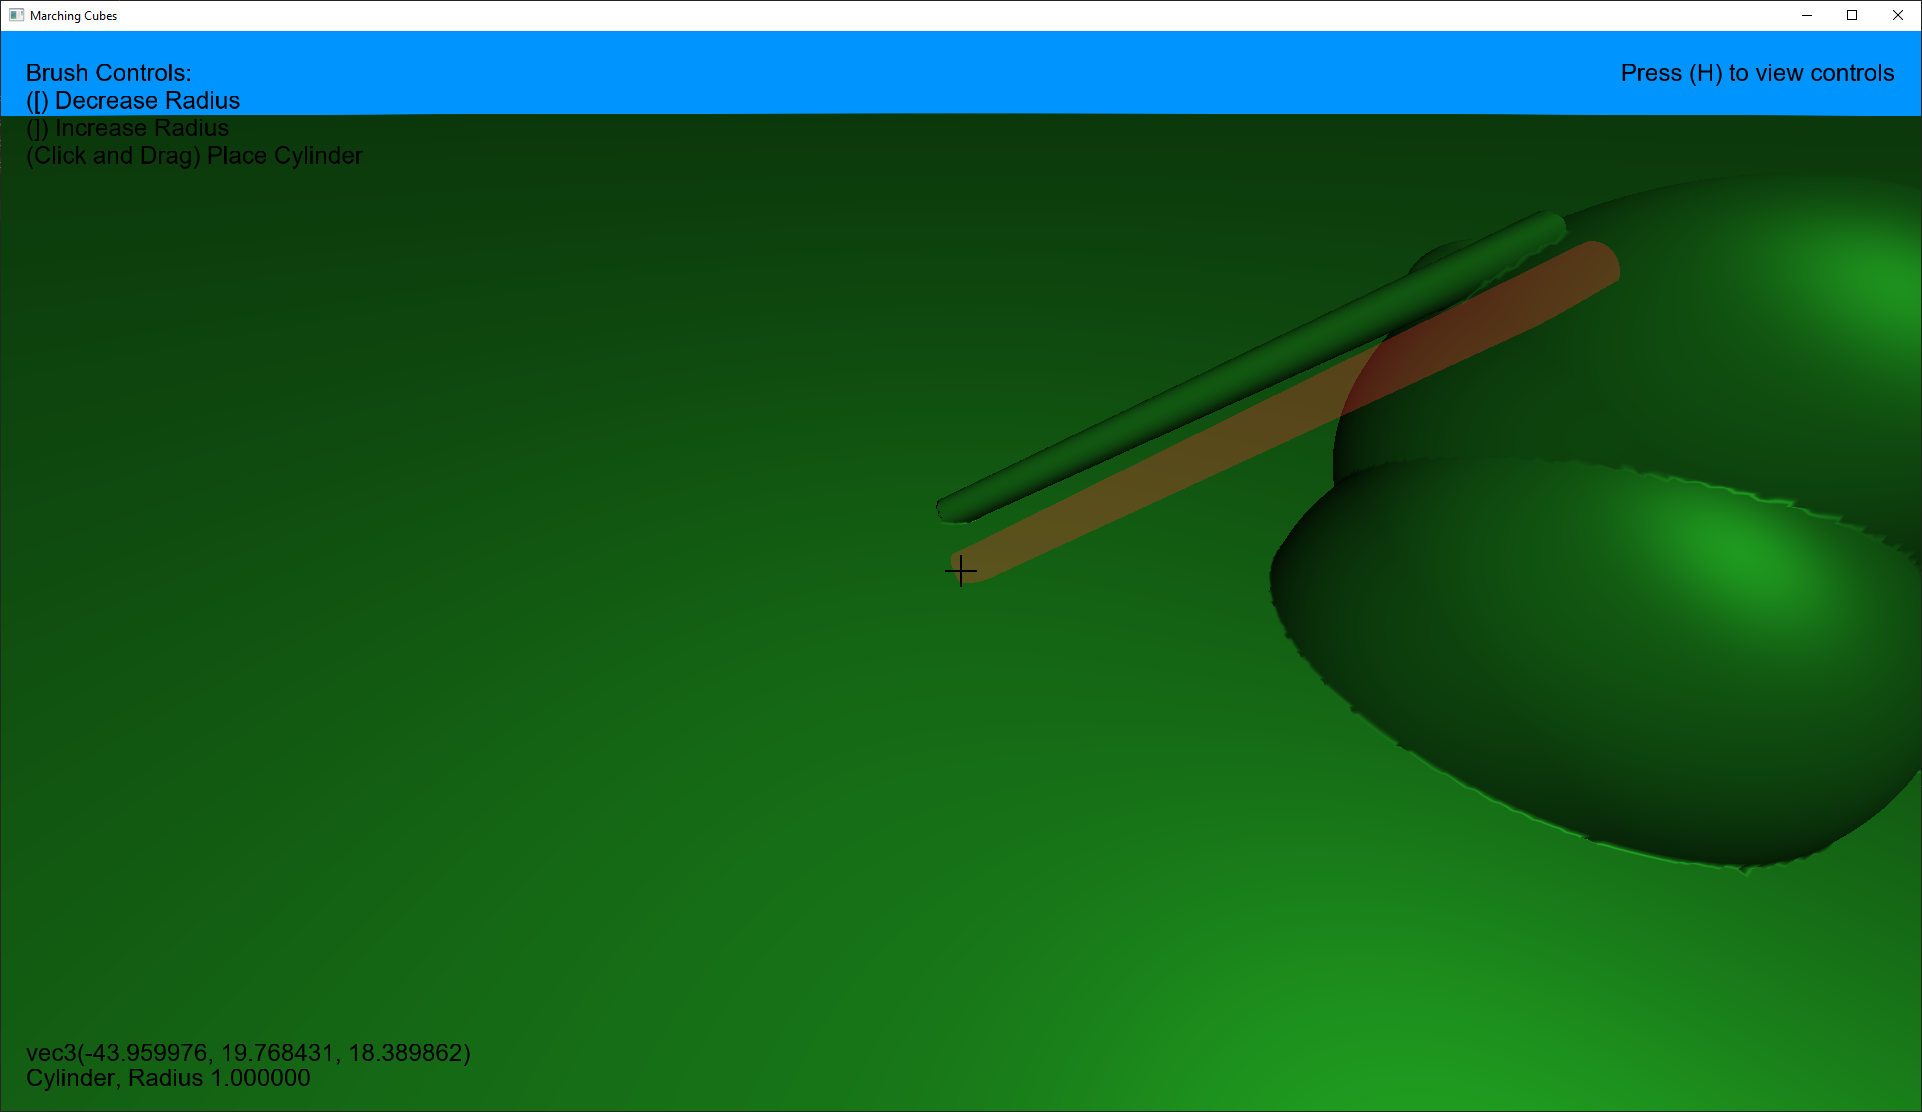
\includegraphics[width=\textwidth]{cylinder_preview.png}
  \caption{Preview of a cylinder about to be placed, next to some shapes which have already been placed.}
  \label{fig:cylinder_preview}
\end{figure}
\begin{figure}[H]
  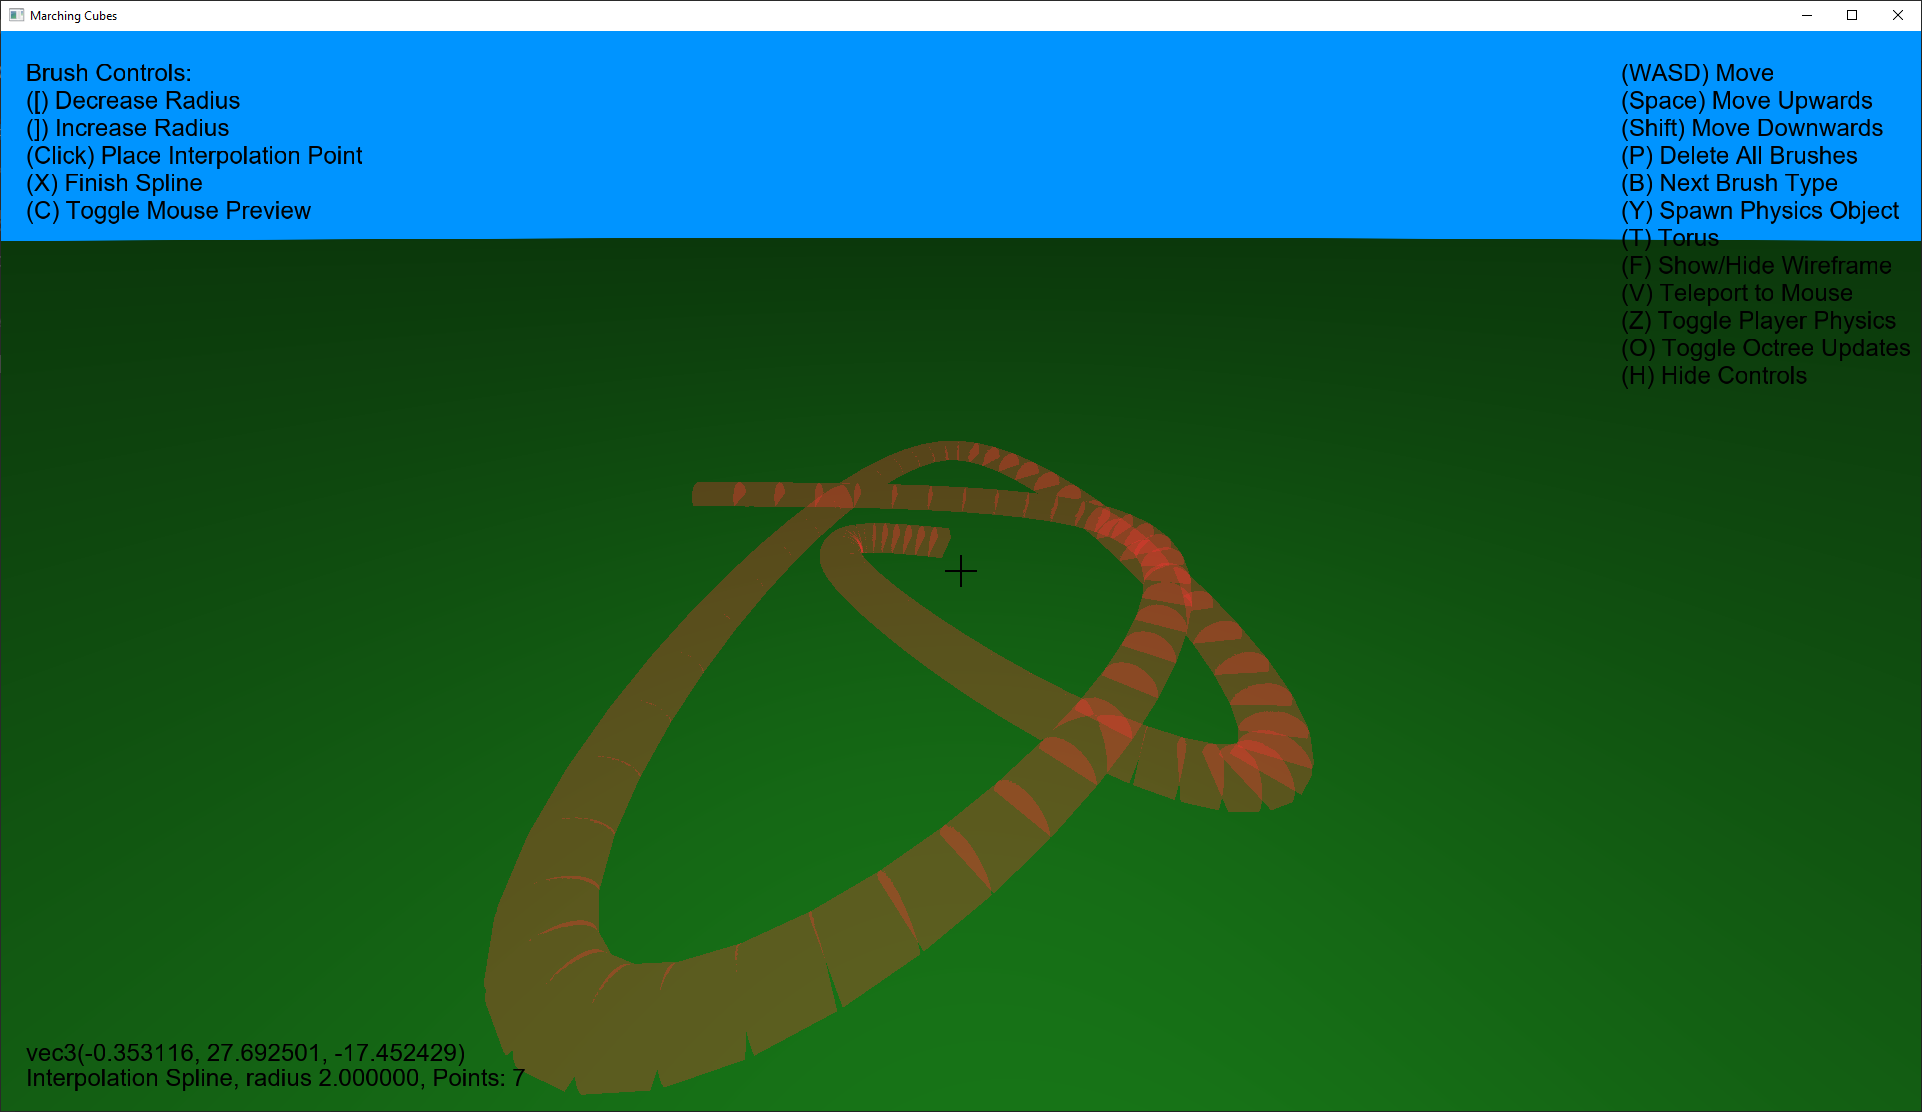
\includegraphics[width=\textwidth]{spline_preview.png}
  \caption{Preview of an interpolation spline with multiple control points. The use of semi-transparent shapes means that visual artifacts are present when the shapes are drawn in a specific order. This can be solved by drawing the shapes in a specific order. However, since the only purpose of rendering this is to display a preview, this is unneccesary.}
  \label{fig:spline_preview}
\end{figure}
\section{Physics}
In many applications it is useful to have collision detection and physics simulation for the terrain. This section explores a method of doing this.
\subsection{Bullet Physics}
To implement physics simulation, we use a library called Bullet Physics~\cite{bullet-physics}, which is a general-purpose CPU based physics library, written in C++.It supports collision detection with static, concave triangle meshes. We will use this functionality, along with the triangle meshes we have already generated, to implement physics simulation.

The library is optimised for speed, and the physics simulation is complex, with multiple different phases used with each timestep. For example, one such phase computes axis-aligned bounding boxes of physics shapes, and returns pairs of objects where these intersect, and a subsequent phase computes the contact points between those objects, using an algorithm chosen based on the types of shape. All of this is encapsulated within a single function, \texttt{stepSimulation}, which takes a time interval, and moves the physics simulation forwards by that amount.

Documentation for the library is automatically generated from source code comments, and as such, is often incomplete and confusing to follow. However, there is a user manual which gives an overview of how some aspects of the library work~\cite{coumans_2015}.

\subsection{Creation of Physics Meshes}
\label{section:physics_meshes}
The geometry we will use for the physics collision meshes is the same geometry used for rendering, generated by the Transvoxel algorithm. We make use of the \texttt{mapGeometry} function, as described in section \ref{section:raycasting}, to copy the geometry to the CPU memory, so it can be accessed by the library.
Creating a concave collision mesh are computationally expensive, and so physics meshes are only constructed on chunks that are generated at the highest level of detail. Figure \ref{fig:meshes1} shows physics meshes being generated in a radius around the camera.

\begin{figure}[H]
  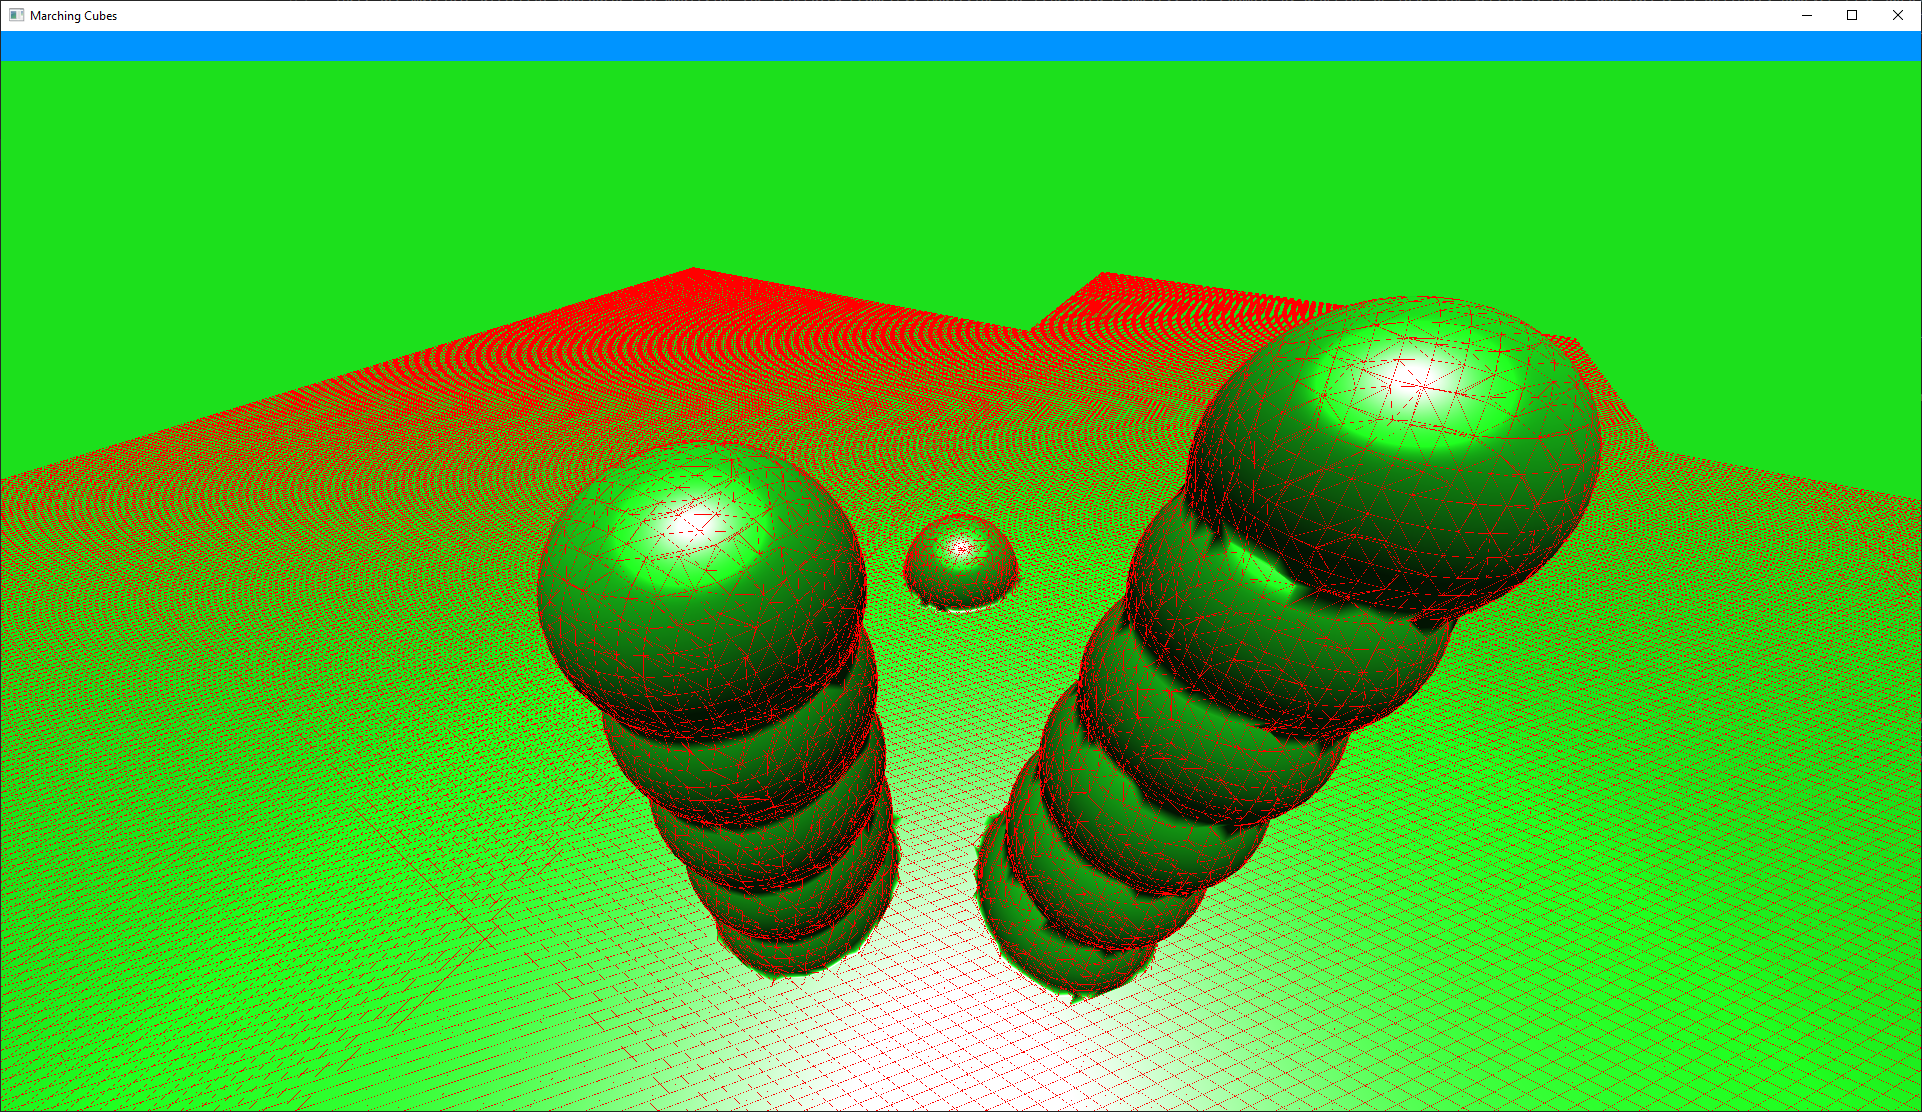
\includegraphics[width=\textwidth]{meshes1.png}
  \caption{Generated physics meshes, shown in red outline.}
  \label{fig:meshes1}
\end{figure}

Making this restriction on the meshes generated means that there are significantly fewer physics meshes being generated with each octree update. This also has the benefit that physics collisions always occur with the same geometry, rather than with geometry at varying levels of detail. If collision with low detail geometry were to occur, finer features in the geometry may be completely ignored. However, this means that collision can only occur where the highest level of detail is used. To solve this, we modify the \texttt{shouldSplit} and \texttt{shouldChop} functions described in section \ref{section:octree}, as shown in listing \ref{phy_lod}.

\begin{lstlisting}[language=C++,label={phy_lod},caption={Snippet from \texttt{shouldSplit} responsible for increasing the level of detail near a set of test physics objects. All chunks with bounding boxes that intersect the bounding box of a physics shape will be split until the highest detail level is reached. The octree refinement process described in section \ref{section:octree_refinement} ensures that this does not create any places where very different levels of detail are adjacent to each other.}]
for (auto shape : TestShape::allShapes) {
  if (getBoundingBox().intersects(shape->getBoundingBox())) {
    return true;
  }
}
\end{lstlisting}

Figures \ref{fig:meshes2} and \ref{fig:meshes3} show this system in action.

\begin{figure}[H]
  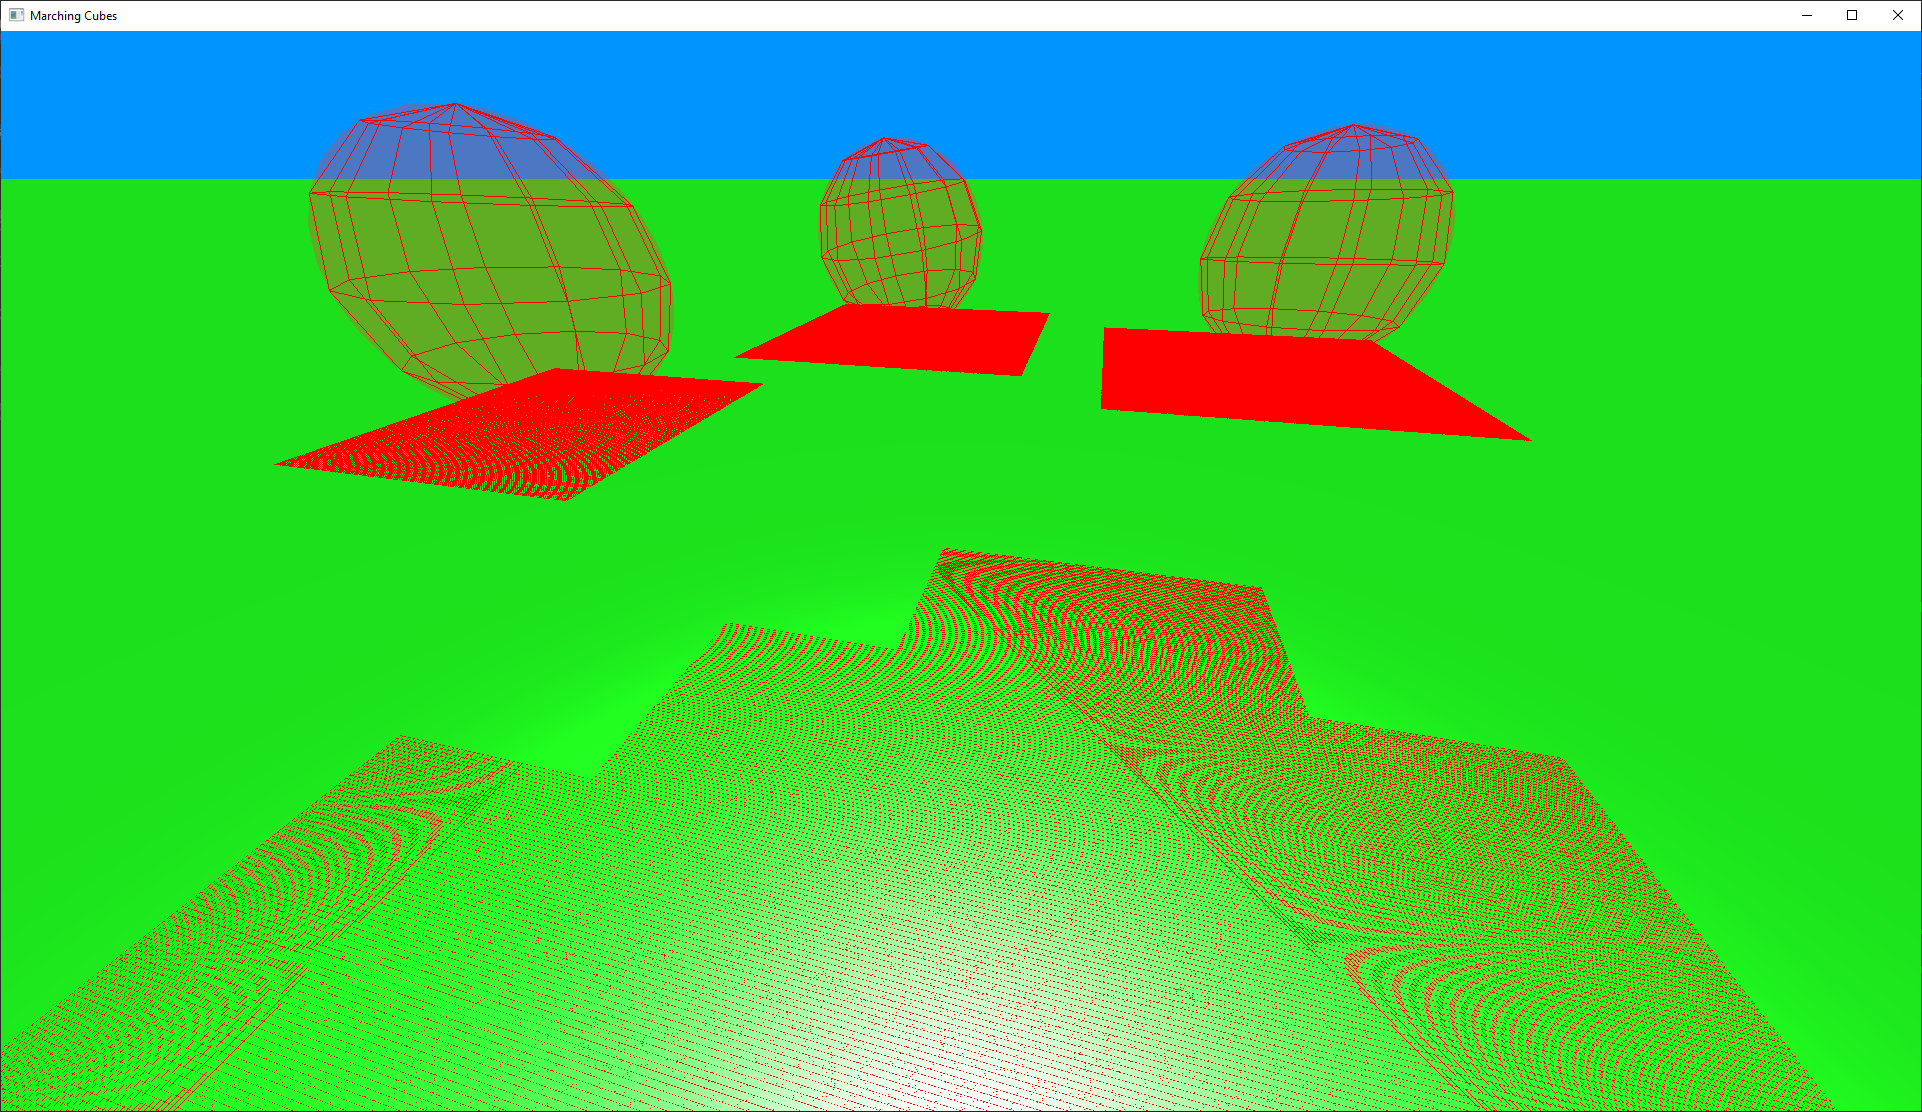
\includegraphics[width=\textwidth]{meshes2.png}
  \caption{Physics meshes generated for large, far away objects. Meshes are shown in red outline. Due to the distance from the camera and the high level of detail, the mesh appears to be rendered as a solid block of color.}
  \label{fig:meshes2}
\end{figure}

\begin{figure}[H]
  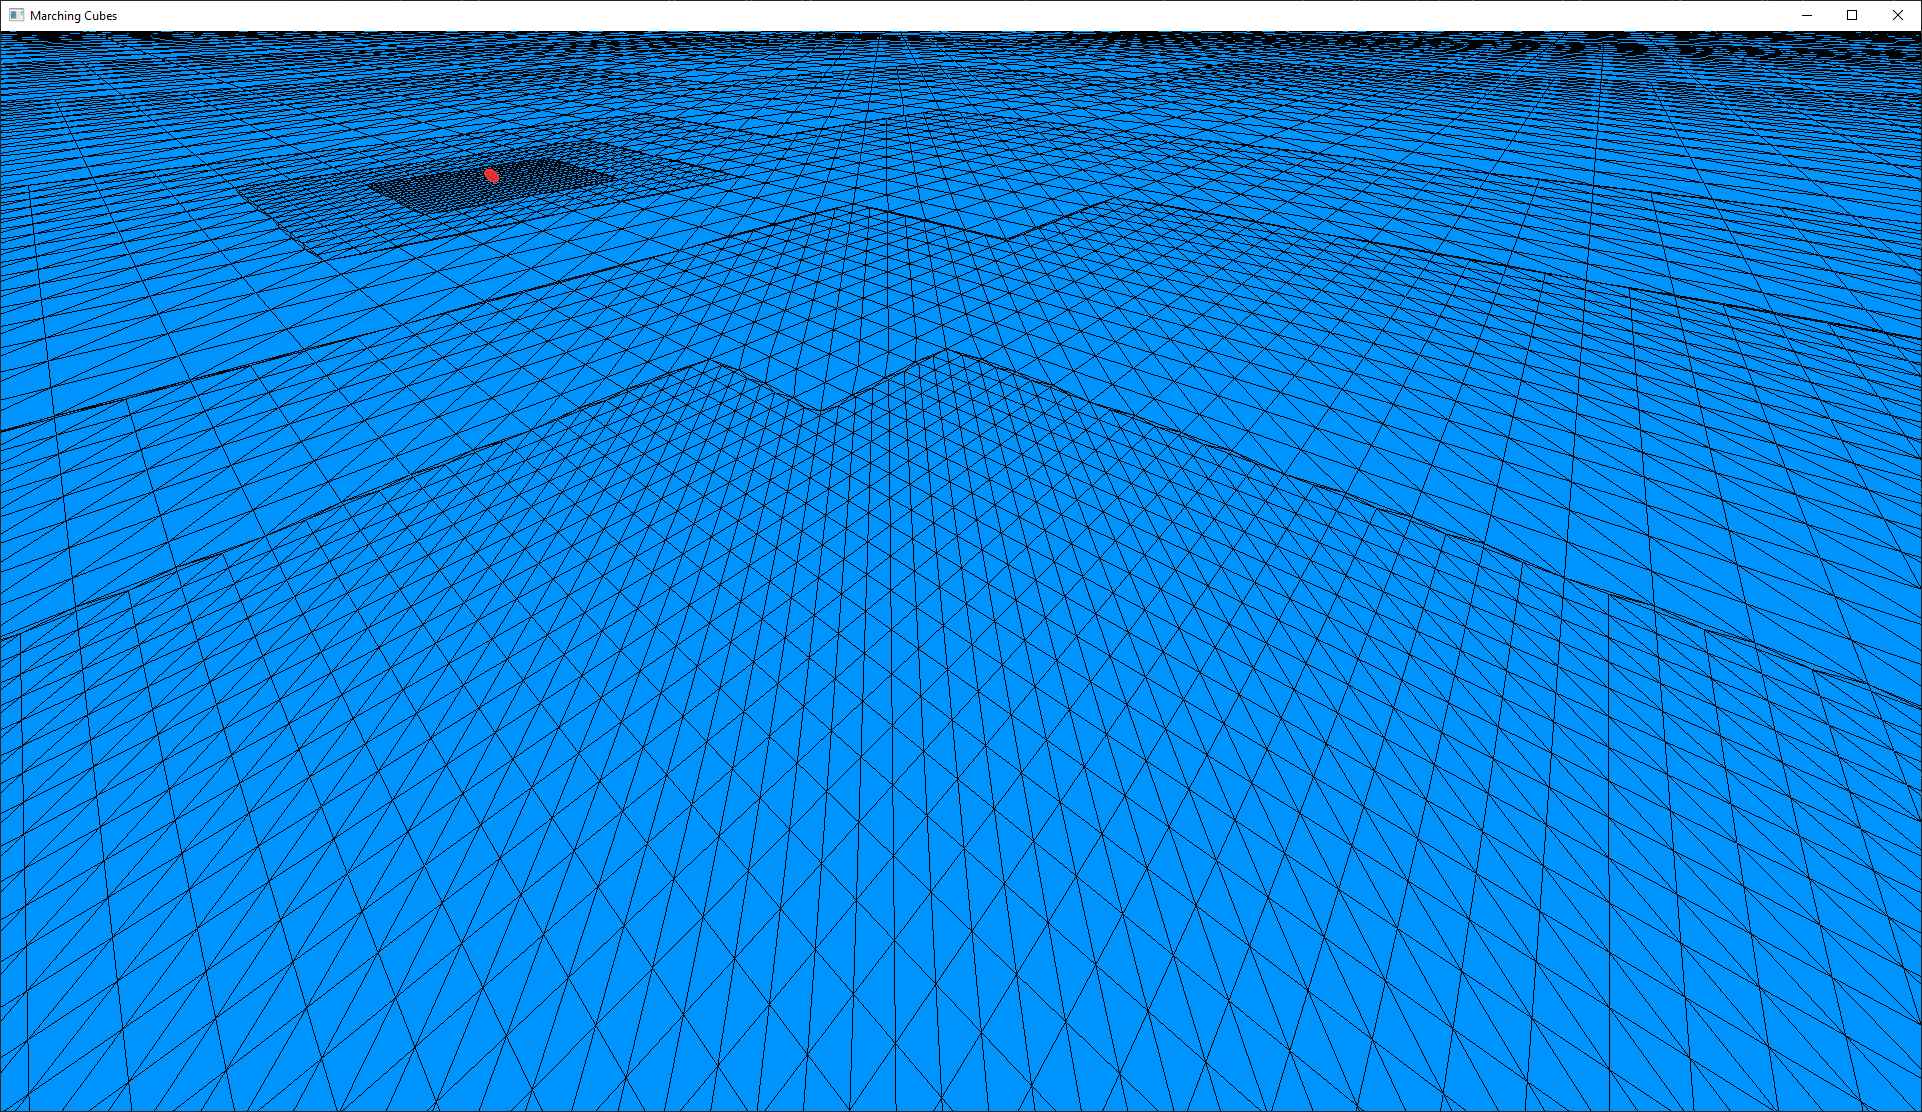
\includegraphics[width=\textwidth]{meshes3.png}
  \caption{Chunk sizes generated for a small, far away physics object. There is no place where a very high level of detail and very low level of detail are adjacent to each other, thanks to the refinement algorithm.}
  \label{fig:meshes3}
\end{figure}

\subsection{Player Controller}
To handle player collision, we use a capsule shape oriented along the y axis, which is moved by applying a force in the direction we want to move. The direction of this force is determined by the directional keys being pressed. For example, if the forward key is being pressed, the shape is pushed horizontally in the direction the camera is looking. The other directional keys act similarly, applying a force relative to the direction of the camera. To move upwards, a large upwards force is applied. 
\subsubsection{Editing geometry near the player}
If geometry is edited near the player, it is possible for the collision shape to become stuck in the collision meshes, or even pass through them entirely, resulting in incorrect collisions. To prevent this from happening, there is the option of a simple camera mode, with no collision detection, and it is possible to restrict terrain editing to only be possible in this mode. In this case, the collision shape is moved to the new position of the camera when the mode is switched again.
\subsection{Multithreading}
\label{section:multithreading}
Even when meshes are only generated for chunks at the highest level of detail, mesh generation for a large chunk of geometry still takes long enough to cause a noticable slowdown. This is because a data structure is created internally for each mesh collision object.

To enable physics meshes to be generated whilst maintaining an interactive framerate, they are generated on a separate thread. All of the information about the collision mesh for a chunk is stored in a \texttt{ChunkMesh} object. There are numerous ways in which race conditions can occur as a result of this multithreading, for example:
\begin{itemize}
  \item A chunk is deleted, whilst a mesh computation that relies on the geometry within is still ongoing on another thread, causing deallocated memory to be read.
  \item A generated physics mesh is added to the simulation by a secondary thread whilst the main thread is performing other calculations to simulate the world, causing errors within the library. This occurs particularly when library functions are iterating over collections of objects already in the simulation, since modifying such collections during iteration can cause unpredictable behaviour. Due to the complexity of the library, it is impractical to anticipate all of the situations where this could occur, and hence we will treat the library function \texttt{stepSimulation} as a black box, only modifying the objects inside the physics simulation within the same thread as this function.
\end{itemize}
To ensure no race conditions of these types occur, the state of a \texttt{ChunkMesh} object is stored in an atomic variable, and carefully maintained throughout its lifetime. Each method that may cause a race condition related to a \texttt{ChunkMesh} object performs an atomic compare-and-swap operation on this variable, to ensure the state remains consistent throughout. There are 7 possible states of a \texttt{ChunkMesh}, and the generation process can be described in terms of this state:
\begin{itemize}
 \item \texttt{CHUNKMESH\_INITIALIZED}: The initial state of a \texttt{ChunkMesh}. On the main thread, the geometry is copied to the CPU, and the object is added to a thread-safe queue \texttt{multiQueue}, which is read by the physics generation threads.
 \item \texttt{CHUNKMESH\_GENERATING}: A physics generation thread removes a \texttt{ChunkMesh} object from \texttt{multiQueue}, changes its state from \texttt{CHUNKMESH\_INITIALIZED} to \texttt{CHUNKMESH\_GENERATING}, and begins executing the expensive library functions responsible for creating the physics object.
 \item \texttt{CHUNKMESH\_FUTURE\_DELETE}: The main thread has attempted to delete the chunk this \texttt{ChunkMesh} belongs to, whilst a physics thread was still working on it. The main thread changes its state from \texttt{CHUNKMESH\_GENERATING} to \texttt{CHUNKMESH\_FUTURE\_DELETE}
 \item \texttt{CHUNKMESH\_GENERATED}: A physics thread has finished the computation for the \texttt{ChunkMesh}, and has changed the state from \texttt{CHUNKMESH\_GENERATING} to \texttt{CHUNKMESH\_GENERATED}. The \texttt{ChunkMesh} object is added to a thread-safe queue \texttt{singleQueue} which is checked regularly by the main thread.
 \item \texttt{CHUNKMESH\_INWORLD}: The main thread removes a \texttt{ChunkMesh} object from \texttt{singleQueue}, adds it to the physics simulation, and changes the state from \texttt{CHUNKMESH\_GENERATED} to \texttt{CHUNKMESH\_INWORLD}.
 \item \texttt{CHUNKMESH\_REMOVING}: A \texttt{ChunkMesh} which was moved to state \texttt{CHUNKMESH\_FUTURE\_DELETE} is moved to \texttt{CHUNKMESH\_REMOVING} instead of \texttt{CHUNKMESH\_GENERATED} when the physics computation finishes. It is also added to \texttt{singleQueue}
 \item \texttt{CHUNKMESH\_REMOVED}: A \texttt{ChunkMesh} is removed from \texttt{singleQueue} by the main thread. If it is in the state \texttt{CHUNKMESH\_INITIALIZED}, then it has not been removed from \texttt{multiQueue} yet, and the expensive computation has not started. The state is changed to \texttt{CHUNKMESH\_REMOVED}, so the computation does not start. If it is in the state \texttt{CHUNKMESH\_INWORLD}, then the mesh has been created, and is currently in the world. The \texttt{ChunkMesh} is removed from the physics simulation and deleted. If it is in the state \texttt{CHUNKMESH\_REMOVING}, then the physics computation has completed, but the mesh is not in the world. The \texttt{ChunkMesh} is deleted.
\end{itemize}

 \begin{figure}[H]
  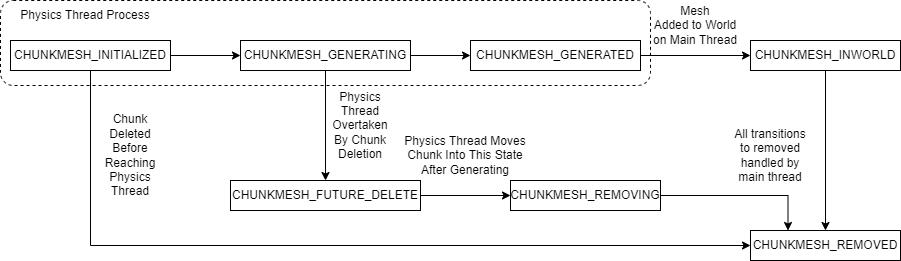
\includegraphics[width=\textwidth]{physics_states.png}
  \caption{States of a physics mesh}
  \label{fig:physics_states}
\end{figure}

\subsection{SDF-Based Physics}
Since all of the geometry is generated using SDFs, there is a possibility of using an SDF for physics simulation, rather than the generated mesh, which is an approximation. In fact, determining whether collision occurs between a sphere and a shape represented by an \textit{exact} SDF is very simple and efficient, requiring only one evaluation of the SDF.

\begin{algorithm}[H]
  \caption{Intersection detection between a sphere and an exact SDF}\label{alg:sdf_sphere_collision}
  \hspace*{\algorithmicindent} \textbf{Input: SDF, p, r} \\
  \hspace*{\algorithmicindent} \textbf{Output:} Whether the sphere centered at \textbf{p} with radius \textbf{r} intersects the surface represented by \textbf{SDF} 
  \begin{algorithmic}
  \If{$\textrm{SDF}\left(p\right) \geq r$} \State\Return false
  \Else \State \Return true
  \EndIf
  \end{algorithmic}
\end{algorithm}

The situation is more complicated with approximate SDFs, since the value of the SDF is no longer guaranteed to be the exact distance from the surface, and so there is no guarantee that moving even a small amount in some direction will not lead to a collision, making this approach ineffective. Figure \ref{fig:approx_collision} shows a 2D example of this.

\begin{SCfigure}[][!h]
  \caption{A circle with radius $0.5$ near an approximate SDF, where the distance is not exact. Here the dashed line is the contour line of the approximate SDF $f\left(x,y\right) = y - \left(1 - \frac{x^2}{3}\right)$ where the value is $0.5$. If this were an exact SDF, then the shapes would only just touch, however they are intersecting.}
  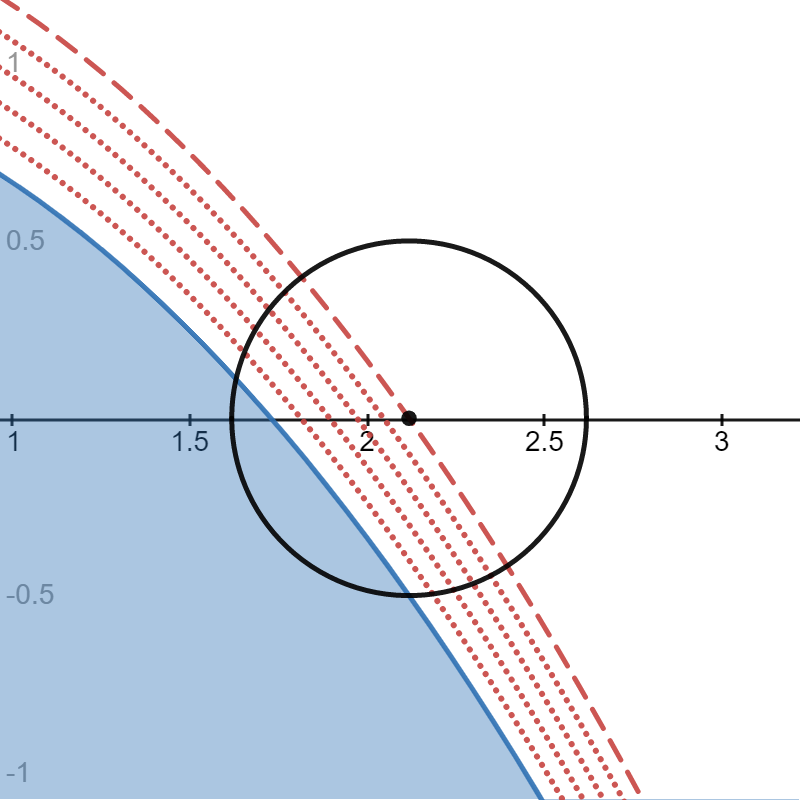
\includegraphics[width=0.5\textwidth]{approx_collision}
  \label{fig:approx_collision}
\end{SCfigure}

Furthermore, collision between an SDF and a different shape is more complicated, even if the SDF is exact. Since the distance from a surface at which a shape is colliding with it is different depending on the orientation of the shape relative to the surface, and the evaluation of an SDF gives no information about direction to the nearest point on the surface, such a system would be inaccurate. This method could still be used with an approximate SDF which provides a lower bound of the distance to the surface, along with a spherical bounding volume for physics shapes, to perform culling on objects to determine when it is impossible for them to intersect. However, we will not explore this here, choosing instead to remain with the library implementation.  

\section{Shading}
A good way to improve the appearance of the generated terrain is to apply some shading. For lighting, we make use of a modified version of Phong lighting, with 2 light sources. We will have a far away light source to represent the sun, with both diffuse and specular reflection. We will also have a light source which is positioned directly above the camera, that only contributes a diffuse component. This gives the appearance that nearby geometry is lighter than geometry that is further away, and excluding the specular component from the player light source prevents everything from appearing as shiny.

\begin{lstlisting}[language=C++,label={lighting},caption={Part of the fragment shader implementing this lighting model.}]
//ambient
float ambientTotal = ambientPower;

//diffuse - from player and from sun
vec4 sunDirection = normalize(sunPos - vertexPosition_worldSpace);

vec4 playerLightPosition = playerLightOffset + vec4(cameraPosition,0.);
vec4 playerLightDirection = normalize(playerLightPosition - vertexPosition_worldSpace);

float diffuseTotal = diffusePower * (
  0.5 * max(0,dot(sunDirection,normalize(vertexNormal_worldSpace))) +
  0.5 * max(0,dot(playerLightDirection,normalize(vertexNormal_worldSpace)))
);

//specular - only from sun
vec4 reflectDirection = reflect(-sunDirection,normalize(vertexNormal_worldSpace));
vec4 cameraDirection = normalize(vec4(cameraPosition,1) - vertexPosition_worldSpace);
float specularTotal = specularPower * pow(max(0,dot(reflectDirection,cameraDirection)),specularExponent);

vec3 terrainColor = (ambientTotal + diffuseTotal + specularTotal) * textureColor;
\end{lstlisting}
We will make use of a customized fragment shader, defining the color of the terrain based on its position and normal using procedural texturing. This has a benefit over using a tiled image, which shows a repeating pattern over a large area, whereas a procedural texture defined using noise will not have such an obvious pattern. Listing \ref{procedural_shading} shows some procedural texturing that appears as grass on horizontal surfaces, and rock on vertical surfaces.

\begin{lstlisting}[language=C++,label={procedural_shading},caption={Part of the fragment shader used to determine the color of each pixel. We use noise to interpolate between different shades of a color, rather than using a flat color. The variable \texttt{grassAmount} determines how much grass is visible at a given point. The noise used to define the rock color has been stretched in the x and z directions. The result is a color that changes more quickly as the y coordinate changes.}]
float grassAmount = smoothstep(0.75,0.9,vertexNormal_worldSpace.y);

//blend factors between 0 and 1, based on 3D noise function of the vertex position
float grassBlend = perlin3(vertexPosition_worldSpace.xyz/10.,octaves);
float rockBlend = perlin3(vertexPosition_worldSpace.xyz/vec3(50.,8.,50.),octaves);

//somewhere between color 1 and color 2, which are different shades of green, gray respectively
vec3 thisGrassColor = mix(grassColor,grassColor2,grassBlend);
vec3 thisRockColor = mix(rockColor,rockColor2,rockBlend);

//mix grass and rock based on grassAmount
vec3 textureColor = grassAmount * thisGrassColor + (1.0-grassAmount) * thisRockColor;    
\end{lstlisting}
Figure \ref{fig:procedural_shading_shapes} shows the shading produced by this algorithm.
\begin{figure}[H]
  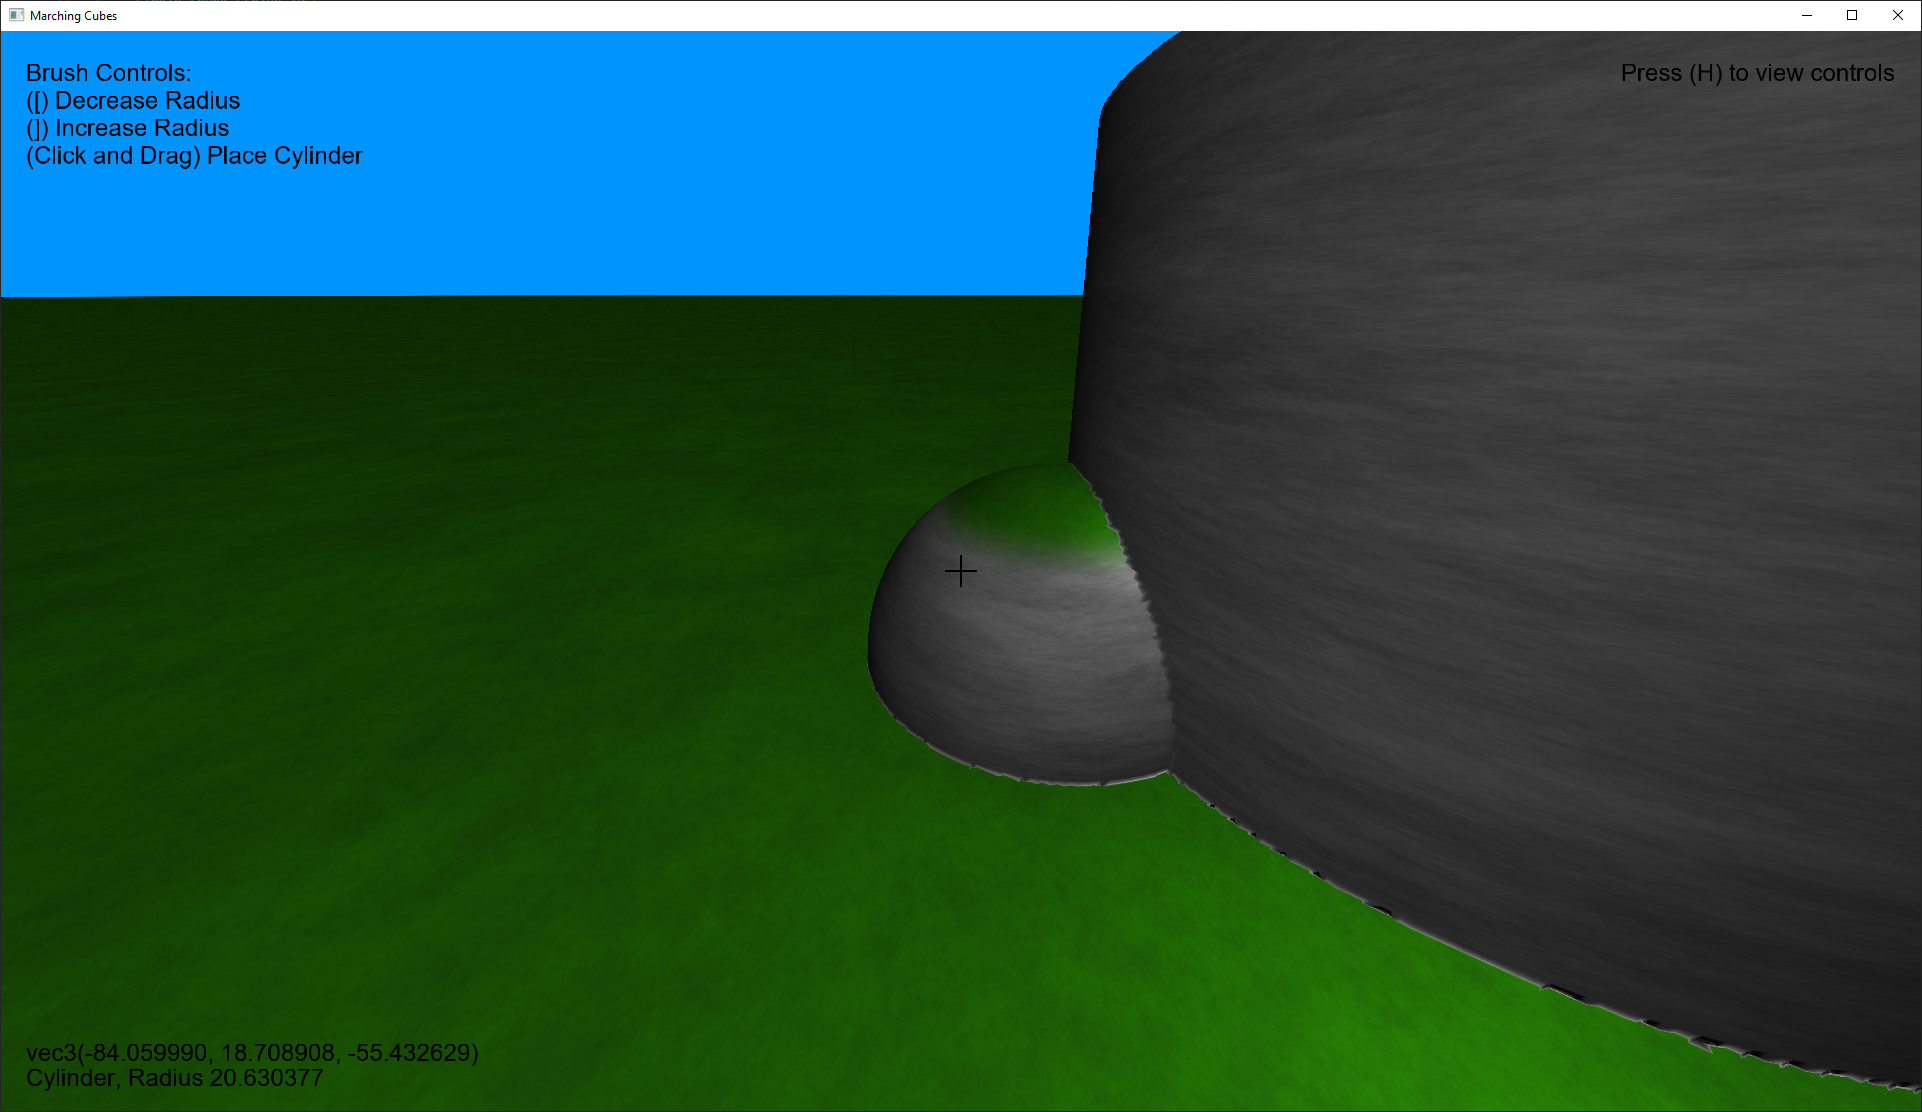
\includegraphics[width=\textwidth]{procedural_shading_shapes.png}
  \caption{Plane, cylinder and sphere, textured using this procedural texturing method.}
  \label{fig:procedural_shading_shapes}
\end{figure}

When these techniques are applied alongside a well-chosen noise-based terrain function, the result is a visually appealing landscape.
\begin{figure}[H]
  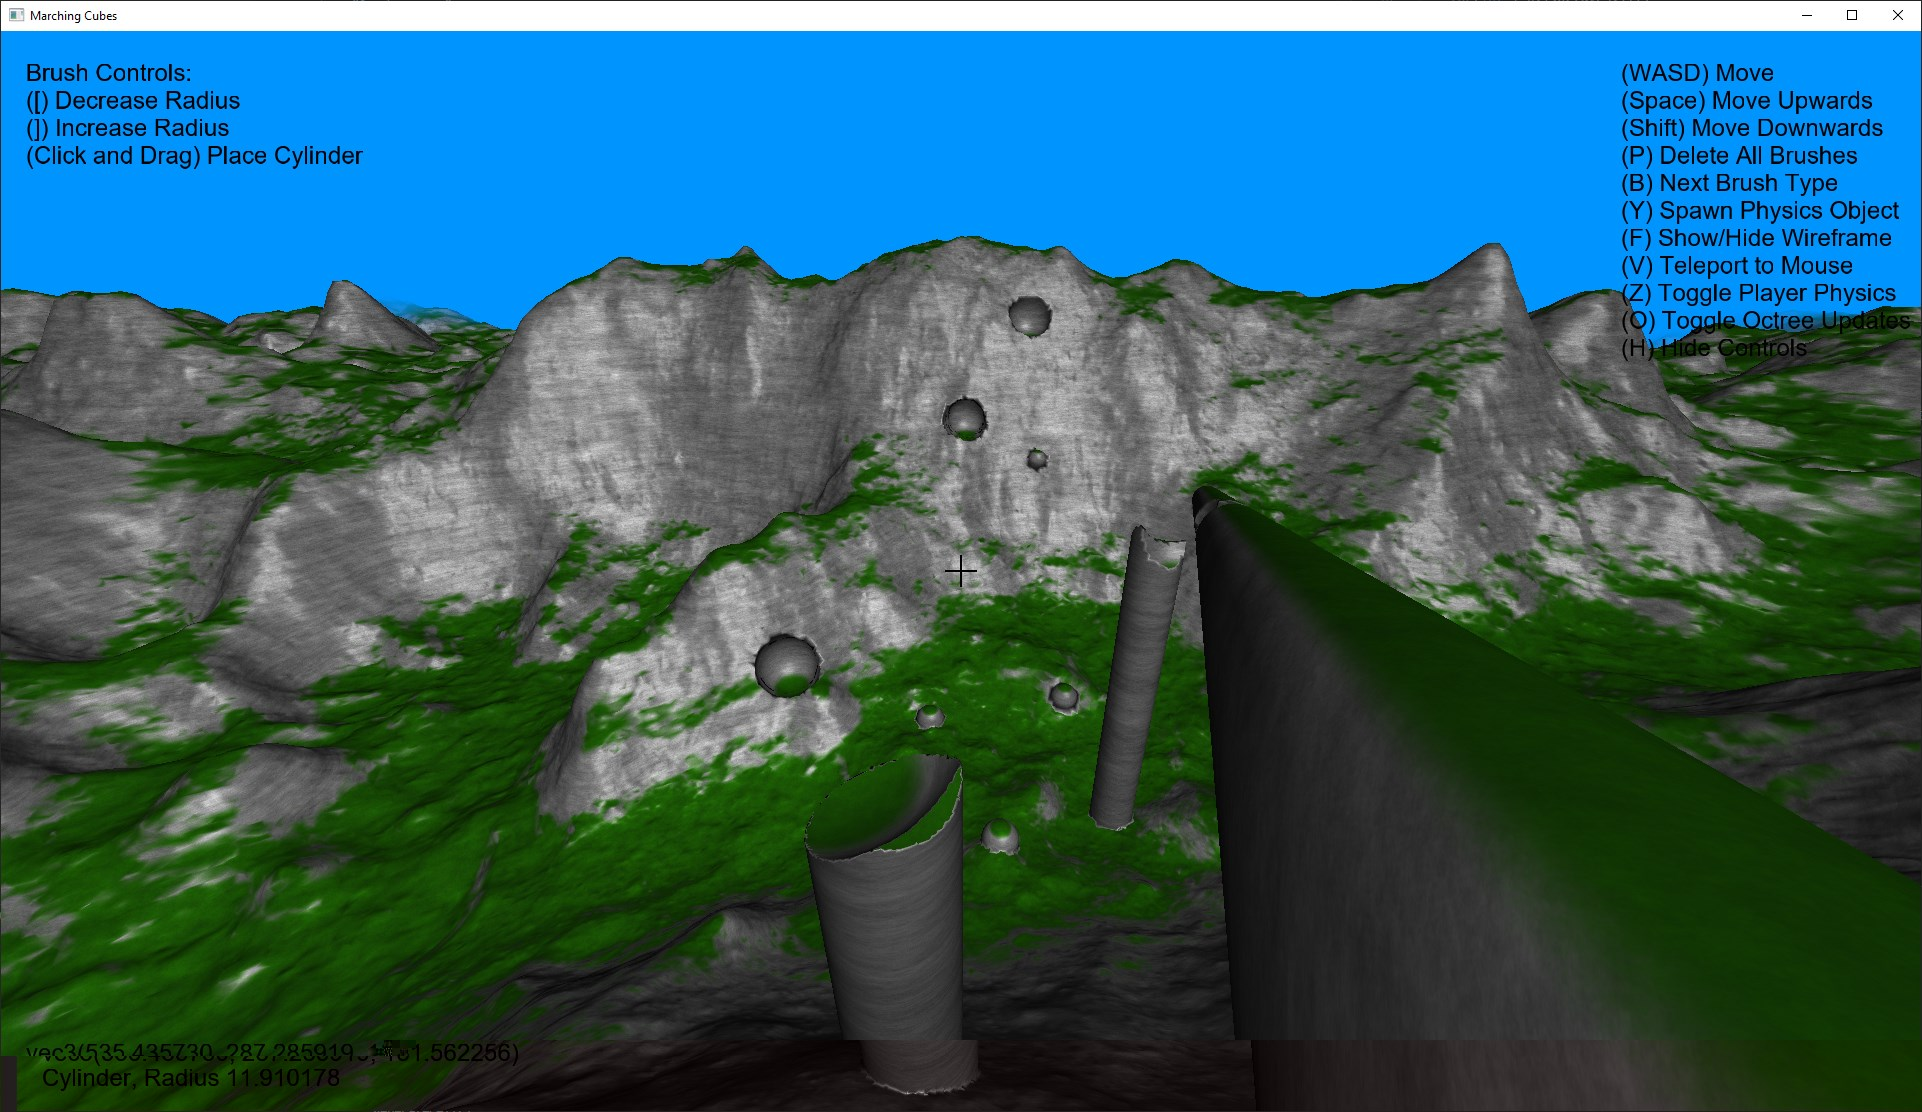
\includegraphics[width=\textwidth]{shaded_mountains.jpg}
  \caption{Mountainous landscape generated using noise, and textured with procedural texturing. }
  \label{fig:shaded_mountainsd}
\end{figure}


\section{Changes in the Implementation}
The code has been iteratively improved over the course of the project. This section briefly explores some of the improvements implemented during development.

\subsection{Storage of Transvoxel sample values}

Each SDF sample value calculated in the first shader stage is stored in a flat buffer, to be retrieved by the later stages. This is implemented with the function \texttt{getArrID} that takes the position of the sample relative to the chunk, and returns an index into the buffer. When the sample points are arranged in a grid, this is relatively simple, however things become more complicated for the sample points in the Transvoxel algorithm, since there are sample points that are midway between the grid cell vertices when transition cells are generated. A simple solution was to double the size of the array in each dimension, so that sample points halfway between grid cells fit in as though the grid size was changed, however this leads to a very sparse buffer that is far larger than it needs to be. A more space-efficient solution stores the sample points not on the faces of the chunk as a cuboid. Then, each face of the chunk is stored at the end of the buffer, so that additional sample points on the face can fit. This results in much less wasted space.

\begin{lstlisting}[language=C++,label={tv_arrID_2},caption={The more efficient \texttt{getArrID} function.}]
  uint getArrID(uvec3 gid, uvec3 halfXYZ) {
    //Store the main volume
    if (gid.x > 0 && gid.x < chunkSize.x &&
        gid.y > 0 && gid.y < chunkSize.y &&
        gid.z > 0 && gid.z < chunkSize.z) {
        return (gid.x - 1) +
               (gid.y - 1) * (chunkSize.x - 1) +
               (gid.z - 1) * (chunkSize.x - 1) * (chunkSize.y - 1); 
    }

    uint offset = (chunkSize.x - 1) * (chunkSize.y - 1) * (chunkSize.z - 1);

    uvec3 temp = 2 * gid + halfXYZ;
    uvec3 ts = 2 * chunkSize + uvec3(1);
    //Store the faces as -x, +x, -y, +y, -z, +z in that order, edges and corners are stored in the first place in this ordering (some unpopulated values)

    //point on the -x face
    if (gid.x == 0 && halfXYZ.x == 0) {
        return offset +
            temp.y + ts.y * temp.z;
    }
    offset += ts.y * ts.z;
    //point on the +x face
    if (gid.x == chunkSize.x && halfXYZ.x == 0) {
        return offset +
            temp.y + ts.y * temp.z;
    }
    offset += ts.y * ts.z;

    //point on the -y face
    if (gid.y == 0 && halfXYZ.y == 0) {
        return offset +
            temp.x + ts.x * temp.z;
    }
    offset += ts.x * ts.z;
    //point on the +y face
    if (gid.y == chunkSize.y && halfXYZ.y == 0) {
        return offset +
            temp.x + ts.x * temp.z;
    }
    offset += ts.x * ts.z;

    //point on the -z face
    if (gid.z == 0 && halfXYZ.z == 0) {
        return offset +
            temp.x + ts.x * temp.y;
    }
    offset += ts.x * ts.y;
    //point on the +z face
    if (gid.z == chunkSize.z && halfXYZ.z == 0) {
        return offset +
            temp.x + ts.x * temp.y;
    }
    offset += ts.x * ts.y;
}
\end{lstlisting}

\subsection{Storage of Editing Brushes}
The first iteration of the editing algorithm stored all brushes for the entire world in one single array, making it simple to add brushes, but meaning that the entire array of brushes had to be iterated through for every chunk, which was prohibitively slow for a large number of brushes, even when individual chunks had a small amount of brushes within them. 

Using the pre-existing octree to store lists of brushes for each chunk, as described in section \ref{section:modification_implementation}, removed the need to do this iteration, at the expense of having to iterate over the octree to add a brush.

\subsection{Bounding Boxes and Grid Cells}
As described in section \ref{section:modification_implementation}, an SDF is only evaluated if the grid cell being worked on intersects its bounding box. A previous iteration only considered whether the sample point was within this bounding box. However, this resulted in incorrect interpolation of geometry vertices in grid cells partially inside the SDF bounding box. This was corrected by extending the bounding box check to include cases where the grid cell intersects the bounding box, even if the sample point does not.

\begin{lstlisting}[language=C++,label={bb_gc},caption={Different iterations of the SDF bounding box check.}]
//Iteration 1 - not considering the entire grid cell
bool inBox(vec4 bottom, vec4 top, vec3 inPos) {
  return all(lessThanEqual(bottom.xyz,inPos)) && all(lessThanEqual(inPos,top.xyz));
}
//Iteration 2 - consider the size of the grid cell when checking
bool inBox(vec4 bottom, vec4 top, vec3 inPos) {
  return all(lessThanEqual(bottom.xyz,inPos + chunkStride)) && all(lessThanEqual(inPos - chunkStride,top.xyz));
}
\end{lstlisting}
  
\section{Conclusion}
\subsection{Reflection}
In this project we have achieved the goal of generating a large area of procedural terrain that can be interacted with in real-time using the Transvoxel algorithm. We showed that parallelising the algorithm on the GPU gives a massive speedup compared to a CPU implementation.

We applied techniques seen in the Geometric Modelling course in interesting ways, using an octree to partition space into regions with different levels of detail, and using interpolation splines as a part of an SDF defining more complex shapes. 
We have also used techniques seen in the Computer Graphics course for handling geometry and rendering 3D images, and from the Concurrent Algorithms and Data Structures course, such as using atomic variables and the compare-and-swap operation to protect against race conditions, in section \ref{section:multithreading}.

At the start of this project, I had some experience working with C++ and the libraries responsible for interacting with OpenGL. The choice of OpenGL as an API was a straightforward one, since it is well-established, and widely supported on modern hardware and operating systems. C++ as a language is also widely used, and compiled code can be very efficient compared to other languages. However, developing in C++ is more challenging than other, higher level languages, with added complexity such as memory management to consider. Developing on Windows, configuring a compiler with libraries introduced throughout development was a source of particular frustration, since each library must be compiled and linked manually. This could be avoided in language that had a more standardised way of including libraries. It would be interesting to implement a similar project in a language such as Python, where bindings for both OpenGL and Bullet Physics exist, comparing the execution speed to the equivalent C++ program.

I particularly enjoyed creating SDFs to represent terrain, and it was satisfying to be able to define a shape using an equation and immediately see it rendered. 

The final implementation contains XXXX lines of code, and can be found at \url{https://github.com/JC-G/Marching-Cubes}.

\subsection{Future Work}
\label{section:future_work}
\subsubsection{Octree Refinement Improvements}
The octree refinement algorithm could be improved when considering physics objects. Currently, only octree leaves that contain physics objects are maintained by the \texttt{shouldChop} function, and all of the leaves that were created by the previous iteration of the refinement algorithm are flagged. Although the flagging means that geometry is not being regenerated every time, this still results in a large amount of unneccesary iteration over the octree as nodes are repeatedly flagged, and then unflagged again.
\subsubsection{Bounding the main SDF}
No equivalent to a bounding box has been implemented for the main SDF. For a simple SDF such as a plane, this would be trivial to implement, however for functions defined by noise, this becomes more difficult, since there could be large regions within the area affected by the SDF, which do not contain any of the surface. This would enable improvements similar to those described in \ref{section:modification_implementation}, preventing SDF computation at a point that is clearly not near the boundary. If every part of the SDF was bounded, it would be possible to completely eliminate computation of the SDF in chunks that were outside of these bounds. 
\subsubsection{Additional Multithreading}
Currently, any geometry generated as a result of an octree update is generated before the next frame is drawn, causing stuttering when a lot of editing is performed, as seen in section \ref{edit_limits}, or when the camera moves very fast. Performing geometry generation and rendering on separate threads would allow for techniques that prevent this slowdown, such as artificially limiting the rate at which new chunks are generated. This would reduce the speed at which the octree can be updated, but would improve the framerate.
\subsubsection{Blends}
Using a blend function rather than set union or subtraction to modify the geometry would reduce the number of places where sharp corners appear in the SDF. However, care would have to be taken that the blend function does not result in geometry being modified outside of the bounding box of the shape being added, or this would result in incorrect generation.
\subsubsection{Terrain Materials}
Alongside a distance and normal function, a material function could also be defined, describing the type of geometry at each point, for example distinguishing between grass and rock. Grid cells could then be shaded by sampling the material function at their vertices. Care would have to be taken when shading cells having different materials at each vertex.

\bibliography{mc}
\end{document}
